%%% index.tex -- Master LaTeX file.
%%%
\documentclass[a4paper,oldfontcommands]{memoir}
\usepackage{prelim2e}

%%% standard utility packages
\usepackage{color}
\usepackage[T1]{fontenc}
\usepackage[final]{graphicx}
%\usepackage[nomsgs]{refcheck}
\usepackage{url}


%%% document appearance and style

\usepackage{beton}
\usepackage{euler}

\usepackage{mdwlist}
%  \renewenvironment{description}{%
%    \begin{basedescript}{%
%        \renewcommand{\makelabel}[1]{\bfseries ##1}%
%      }%
%    }{%
%    \end{basedescript}%
%  }
%\usepackage{mdwtab}
\usepackage[newitem,newenum]{paralist}
  \setdefaultenum{\slshape (1)}{\slshape (a)}{\slshape (i)}{A.}
  %\setdefaultitem{\blacktriangleright}{\smalltriangleright}{$\bullet$}{$\circ$}
  \setdefaultitem{\guillemotright}{\guilsinglright}{$-$}{*}


%%% specialized utilities

\usepackage{fancyvrb}
  \DefineShortVerb{\"}

\usepackage[final]{listings}%
  \def\codefont{\ttfamily}%
  \newcommand\q[1]{{\codefont #1}}%
  \newcommand\qq[1]{`\q{#1}'}%
  \lstloadlanguages{Python}%
  \lstset{language=Python,%
          %fancyvrb,%
          escapechar=|,% "|" is almost unused in Python
          basicstyle=\codefont,%
          commentstyle=\normalfont\small,%
          texcl,mathescape=true,%
          showspaces=false,%
          showstringspaces=false,%
          xleftmargin=2em,%
          numbers=left,%
          numberstyle=\tiny,%
          stepnumber=1,%
          firstnumber=last%
        }%
  \lstnewenvironment{code}{}{}%
  \lstnewenvironment{codexmp}{\lstset{numbers=none,xleftmargin=1em}}{}%
  \newcommand{\n}[1]{\begingroup\def\x{\csname label\endcsname{l:#1}}\x\endgroup}
  \newcommand{\nr}[1]{\begingroup\def\x{\csname ref\endcsname{l:#1}}\x\endgroup}

% \usepackage[debug]{csref}
%   \newcsref{theorem}{Theorem~\ref{#1}}%
%   \newcsref{lemma}{Lemma~\ref{#1}}%
%   \newcsref{proposition}{Proposition~\ref{#1}}%
%   \newcsref{claim}{Claim~\ref{#1}}%
%   \newcsref{conjecture}{Conjecture~\ref{#1}}%
%   \newcsref{example}{Example~\ref{#1}}%
%   \newcsref{definition}{Definition~\ref{#1}}%
%   \newcsref{corollary}{Corollary~\ref{#1}}%
%   \newcsref{remark}{Remark~\ref{#1}}%

%% package FIXME
\makeatletter%
\newcounter{fixme@note}\stepcounter{fixme@note}%
\newcommand{\FIXME}[1]{%
  \begingroup%
    \def\thefootnote{\fnsymbol{footnote}}%
    \colorbox{red}{\footnotemark[\value{fixme@note}]}%
    \footnotetext[\value{fixme@note}]%
    {\sffamily \colorbox{red}{FIXME:} #1}%
  \endgroup%
  \stepcounter{fixme@note}%
}%
\makeatother%

\usepackage[ps,dvips,xdvi,colour,all,arc,knot,poly]{xy}
  \everyxy={/r24pt/:} % scala per i diagrammi
  \def\xyc#1\endxyc{\xy*!LC\xybox{#1}\endxy}

\usepackage{rg} % vertici e buche di grafi a nastro

\usepackage{xytree}
\setlength{\treegap}{24pt}  
\setlength{\treeheight}{18pt}


%%% mathematics
\usepackage[reqno]{amsmath}

\usepackage{amsthm}
\providecommand{\theoremname}{Theorem}

\newtheorem{theorem}{Theorem}[chapter]
\newtheorem*{theorem*}{Theorem}
\newtheorem{lemma}[theorem]{Lemma}
\newtheorem{proposition}[theorem]{Proposition}
\newtheorem{claim}[theorem]{Claim}
\newtheorem{conjecture}[theorem]{Conjecture}
\newtheorem{corollary}[theorem]{Corollary}

\theoremstyle{definition}
\newtheorem{definition}[theorem]{Definition}
\newtheorem{example}[theorem]{Example}

\theoremstyle{remark}
\newtheorem{remark}[theorem]{Remark}
\newtheorem*{ack}{Acknowledgments}
\newtheorem*{notations}{Notations}

\numberwithin{equation}{section}


%%%
%%% NOTAZIONI MATEMATICHE
%%%

\usepackage{miscmath} % simboli vari

\providecommand{\textsubscript}[1]{$\sb{#1}$}
\providecommand{\textsuperscript}[1]{$\sp{#1}$}

\renewcommand\k\fk % campo k
\renewcommand\d\ud % differenziale d

\newcommand{\ksz}{\epsilon} % segno di koszul
\newcommand{\aksz}{\chi}    % segno di koszul alternante

\newcommand{\A}{\category{A}}     % generic category A
\newcommand{\B}{\category{B}}     % generic category B
\newcommand{\rev}{\sptext{rev}}
\newcommand{\catN}{\category{N}}        % generic category N

\newcommand{\freemc}[1]{#1^{\otimes}}   % free monoidal category 
\newcommand{\freemsc}[1]{#1^{\Box}}     % free monoidal signed category 
\newcommand{\tpc}[1]{\langle #1 \rangle}% tensor powers category
\newcommand{\btpc}[1]{\langle#1\rangle^+}% (bosonic) tensor powers category

\newcommand{\Oo}[1][]{\operad{O}_{#1}}  % generic operad O
\newcommand{\Ao}{\operad{A}}            % associative operad A
\newcommand{\RTD}[1][]{\operad{D}_{#1}} % operad of RT diagrams
\newcommand{\RTE}[1][]{\operad{D}'_{#1}}% operad of embedded RT graphs
\newcommand{\RTG}[1][]{\operad{G}_{#1}} % operad of RT graphs
\newcommand{\RG}{\operad{R}}            % operad of cyclic (Ribbon) graphs
\newcommand{\ERG}{\operad{\widetilde R}}% operad of embedded Ribbon graphs
\newcommand{\SG}[1][]{\operad{S}_{#1}}  % operad of symmetric graphs

\newcommand{\Strebel}[1][]{\mathcal{S}_{#1}}
\newcommand{\Conf}{\text{\rm Conf}}
\newcommand{\Lb}{\mathcal{L}}
\newcommand{\Hn}{\mathcal{H}}

\newcommand{\Harmonic}{\mathcal{H}} % space of harmonic functions

\newcommand{\ad}{\textrm{ad}} % adjoint action ad[X,Y]

% decomposizione cellulare dei grafi a nastro
\newcommand{\Vertices}[1]{V(#1)}
\newcommand{\Edges}[1]{E(#1)}
\newcommand{\Legs}[1]{L(#1)}
\newcommand{\Holes}[1]{B(#1)}

\newcommand{\comb}{\sptext{comb}}
\newcommand{\T}{\mathcal{T}}
\newcommand{\Tcomb}{\T\comb}
\newcommand{\M}{\mathcal{M}}       % spazio dei moduli di curve lisce
\newcommand{\Mbar}{\overline{\M}}  % compattificazione
\newcommand{\Mcomb}{\M\comb}       % triangolazione di Mumford-Harer
\newcommand{\Mbarcomb}{\Mbar\comb}

\newcommand{\R}{\mathcal{R}}       % complesso dei grafi a nastro


\newcommand{\Hermitian}[1][\relax]
  {\mathcal{H}}   % spazio delle matrici hermitiane
%  {{\mathcal{H}\ifx#1\relax\else(#1)\fi}}   % spazio delle matrici hermitiane


% spazi negativi
\newcommand{\negquad}{\hskip-.5em\relax}
\newcommand{\negqquad}{\hskip-1.5em\relax}


% medie sui grafi
\newcommand{\expval}[1]{\langle\!\langle#1\rangle\!\rangle}
\newcommand{\X}{\mathcal{X}}
\newcommand{\vv}[1]{V(#1)}
\newcommand{\biggint}[2][]{%
\Biggl\langle\Biggl\langle#2\Biggr\rangle\Biggr\rangle_{#1}}
\newcommand{\gint}[2][]{%
  \left\langle\!\left\langle#2\right\rangle\!\right\rangle_{#1}}
\newcommand{\ginttriv}[2][]{%
  \left\langle\!\left\langle#2\right\rangle\!\right\rangle_{#1}\triv}

% decomposizione ciclica
\newcommand{\dec}{\sbtext{\rm dec}}
\newcommand{\res}{\sbtext{\rm res}}

% omotopia
\newcommand{\rel}{\sim}


%%% hyperref
%\usepackage{hyperref}


%%% document
\includeonly{algorithm,python}
\begin{document}
\VerbatimFootnotes% from `fancyvrb`

\setlength{\parindent}{0pt}
\setlength{\parskip}{2ex plus 0.5ex minus 1ex}


\frontmatter

%auto-ignore


\title{%
  Computational techniques in Graph Homology \\
  of the Moduli Space of Curves
}
\date{\today}
\author{Riccardo Murri}
\address{%
  CSCS - Centro Svizzero di Calcolo Scientifico \\
  via Cantonale, 1 \\
  CH-6928 Manno \\
  Switzerland
}
\email{riccardo.murri@gmail.com}

%\subjclass{To be determined}
%\begin{abstract}
%\end{abstract}
\maketitle

\setcounter{tocdepth}{2} % fino a profondit{\`a} di \section

\tableofcontents

%%% Local Variables: 
%%% mode: latex
%%% TeX-master: "index"
%%% End: 



\mainmatter

\RCSID $Id: prelim.tex,v 1.2 2003/06/23 17:38:08 murri Exp $
%auto-ignore


\chapter{Preliminaries and Notation}

This chapter fixes some notations on differential graded modules
and miscellaneous categories.\FIXME{Bof!} 

When $\A$ is a category, we shall use Eilenberg's $\A(A, B)$ in place
of the more verbose $\Hom \A(A, B)$; also, the words ``morphism'',
``map'' and ``arrow'' will be used interchangeably. By abuse of
notation, we write $A \in \A$ to mean that ``$A$ is an object of
$\A$''. Often, the notation $\Hom\A$ will be used for the union of all
the $\Hom$-sets of the category $\A$, i.e., $\Hom\A := \bigcup_{A,B \in \A}
\A(A,B)$.

The symbol $\Perm{k}$ stands for the group of permutations on $k$
letters.

The degree $i$ component of a graded object $M$ will be denoted
$M^i$; the grading group will always be $\setZ$. Elements of a graded
object appearing as exponents to a number will stand for their degree,
i.e., $(-1)^a := (-1)^{\deg a}$; therefore, $(-1)^{ab} \not=
(-1)^{\deg (ab)} = (-1)^{\deg a + \deg b}$.


\section{Differential graded algebras and modules}
\label{sec:dg-things}

Let $\fk$ be a fixed field of characteristics $0$; later on, we shall
assume $\fk = \setC$.
\begin{definition}
  A dg-algebra $K$ is given by the following data of a graded vector
  space $K^\#$ over $\fk$, a $\fk$-bilinear associative product, and a
  $\fk$-linear map $\ud: K\to K$ such that:
  \begin{enumerate}
  \item $K^i \cdot K^j \subset K^{i+j}$;
  \item $ab = (-1)^{ab} ba$ (graded commutativity);
  \item $\ud(K^i) \subset K^{i+1}$;
  \item $\ud(a\cdot b) = \ud(a)\cdot b + (-1)^a a\cdot\ud(b)$ (graded Leibniz rule).
  \end{enumerate}
  Furthermore, we shall always assume that a dg-algebra has a unit
  $1\in K^0$ such that $1\cdot a = a\cdot 1 = a$ for all $a\in
  K$.
\end{definition}

Any dg-algebra is a (graded) associative commutative algebra; write
$\#$ for the underlying functor that ``forgets the differential''.

\begin{definition}
  A $K$-dg-module $M$ is a $K$-bimodule such that:
  \begin{enumerate}
  \item $K^i M^j \subset M^{i+j}$, $M^i K^j \subset M^{i+j}$;
  \item $\lambda x = (-1)^{\lambda x} x\lambda$, for all homogeneous
    $x\in M$, and $\lambda\in K$;
  \item $\ud(\lambda x) = \ud(\lambda)x + (-1)^\lambda \lambda\ud(x)$.
  \end{enumerate}
\end{definition}

There is an obvious underlying functor $\#$ from the category of
$K$-dg-modules to the category of $K$-modules.

\begin{definition}
  For every two $K$-dg-modules $M$, $N$ we define the module of
  degree $p$ morphisms
  \begin{equation*}
    \Hom_K^p (M,N) := \Bigl\{ f\in  {\textstyle \prod_i} Hom_\fk (M^i, N^{i+p}) :
      f(x\lambda) = f(x)\lambda \quad \forall x\in M, \forall \lambda
      \in R \Bigr\},
  \end{equation*}
  and the graded module of morphisms
  \begin{equation*}
    \Hom_K^* := \oplus_{p\in\setZ} \Hom_K^p (M,N)[-p],
  \end{equation*}
  that is, $\Hom_K^p(M,N)$ is the degree $p$ component of
  $\Hom_K^*(M,N)$.
\end{definition}

$\Hom_K^*(M,N)$ is made into a $K$-dg-module by the differential:
\begin{equation*}
  \ud f := \ud_N \circ f + (-1)^{p+1} f\circ \ud_M \qquad f\in \Hom_K^p(M,N)
\end{equation*}
The term ``morphism'' will denote any element of $\Hom_K^*$, whereas
``dg-morphism'' will be applied only to those such that $\ud f = 0$.


\section{Braided symmetric categories of Modules}
\label{sec:btc+dg}

Given any commutative dg-algebra $K$, the category $\catMod_K^\setZ$ of
finitely-generated dg-K-bimodules is in a natural way braided and
balanced with the structure maps:
\begin{align}
  \label{eq:dgm-braiding}
  \tau_{MN} &: M \otimes N \ni m\otimes n \mapsto (-1)^{mn}n\otimes m \in N \otimes M
  &&
  \text{(braiding),}
  \\
  \label{eq:dgm-balancing}
  \theta_M &: M \ni m \mapsto (-1)^mm \in M
  &&
  \text{(balancing).}
\end{align}
The verification that these maps satisfy the axioms of a balanced
braided symmetric category is an easy calculation.  The usual
definition of the dual object $\rdl{M} := \Hom_K(M, K)$ gives an
obvious evaluation map $\ev_M : M \otimes \rdl{M} \ni m \otimes \rdl{m} \mapsto
\pairing{m}{\rdl{m}} \in K$, but we cannot guarantee the existence of a
matching coevaluation morphism unless $M$ is a free module.

The above structure maps
\eqref{eq:dgm-braiding}--\eqref{eq:dgm-balancing} induce a balanced
symmetric braided category structure on the subcategory $\catMod_K$ of
degree $0$ $K$-bimodules; note that the braiding on $\catMod_K$ is the
trivial one: $\tau_{MN}: m\otimes n \mapsto n\otimes m$.
\begin{remark}
  In fact, Eilenberg-Kelly \cite{eilenberg-kelly;monoidal-categories}
  show that there are just two possible braidings on $\catMod_K^\setZ$:
  the trivial one given by
  \begin{equation*}
    \tau_{MN}^+ : m\otimes n \mapsto n\otimes m,
  \end{equation*}
  which is the usual braiding on categories of non-graded modules and
  vector spaces, and and that of \eqref{eq:dgm-braiding},
  \begin{equation*}
    \tau_{MN}^- : m\otimes n \mapsto (-1)^{mn} n\otimes m,
  \end{equation*}
  which is the usual one on categories of graded modules.
\end{remark}


\section{Signs and the graded contraction}
\label{sec:signs}

Recall that the symmetric monoidal category of graded modules has a
non-trivial (yet involutive) twisting isomorphism
\begin{equation*}
\tau_{(12)} = \tau_{M_1M_2} : M_1
\otimes M_2 \ni x_1\otimes x_2 \mapsto (-1)^{x_1x_2} x_2\otimes x_1
\in M_2\otimes M_1,
\end{equation*}
for all objects $M_1$, $M_2$. For any
$\sigma\in\Perm{n}$, there's an isomorphism $\tau_\sigma$ between
$M_1\otimes \dots \otimes M_n$ and $M_{\sigma_1} \otimes \dots
\otimes M_{\sigma_n}$ made up of twists $\tau_{(ij)}$; since the
category of graded modules is \emph{symmetric}, any two such
compositions are equal, that is, $\tau_\sigma$ depends only on
$\sigma\in\Perm{n}$.

Now, suppose $M_1 = \dots = M_n = M$, a fixed object: $x_1\otimes
\dots \otimes x_n$ and $\tau_\sigma(x_1\otimes
\dots \otimes x_n)$ differ only by the sign; therefore we define
$\epsilon(\sigma; x_1, \dots, x_n)$ so that the following holds:
\begin{equation}
  \label{eq:ksz}
  \epsilon(\sigma; x_1, \dots, x_n) x_1 \otimes \dots \otimes x_n =
  \tau_\sigma (x_1 \otimes \dots \otimes x_n), \qquad \sigma\in\Perm{n}.
\end{equation}
Also define $\chi(\sigma; x_1, \ldots, x_n)$ by:
\begin{equation}
  \label{eq:aksz}
  \chi(\sigma; x_1, \dots, x_n) x_1 \otimes \dots \otimes x_n =
  (-1)^\sigma \tau_\sigma (x_1 \otimes \dots \otimes x_n), 
  \qquad \sigma\in\Perm{n}.
\end{equation}
We shall omit $x_1, \dots, x_n$ from the above when it will be clear
from the context which elements $\epsilon$ or $\chi$ are being
applied to.

\begin{definition}\label{dfn:graded-sym-map}
  A map $f: M^{\otimes n} \to N$ is graded symmetric iff
  \begin{equation*}
    f(x_1, \dots, x_n) = \epsilon(\sigma) f(x_{\sigma_1}, \dots,
    x_{\sigma_n}) \qquad \forall x_1, \dots, x_n \in M.
  \end{equation*}
  It is graded antisymmetric iff
  \begin{equation*}
    f(x_1, \dots, x_n) = \chi(\sigma) f(x_{\sigma_1}, \dots,
    x_{\sigma_n}) \qquad \forall x_1, \dots, x_n \in M.
  \end{equation*}
\end{definition}

Since permutation of factors in a tensor product may change the sign,
the contraction map 
\begin{equation*}
c: {\textstyle \bigotimes_i} \Hom(M_i, N_i) \otimes
 {\textstyle \bigotimes_i} M_i \to  {\textstyle \bigotimes_i} N_i
\end{equation*}
is well-defined only up to a sign. In search of a remedy, we fix an
ordering of the factors which gives ``unsigned'' contraction, and then
define contraction of any permutation of the factors
$\left\{\Hom(M_i,N_i), M_i\right\}_{i\in I}$ by first applying a
twist $\tau_\sigma$ to get the fixed ``standard'' ordering, and then the
contraction before. Formally, let:
\begin{enumerate}
\item $\Hom(M,N) \otimes M \ni f\otimes x \mapsto f(x) \in N$;
\item $\bigotimes_i (\Hom(M_i, N_i) \otimes M_i) \ni (f_1\otimes x_1)
  \otimes \dots (f_k\otimes x_k) \mapsto f_1(x_1) \otimes \dots
  \otimes f_k(x_k) \in \bigotimes N_i$;
\item let $W_{2i-1} := \Hom(M_i, N_i)$, $W_{2i} := M_i$, for $i =
  1, \dots, k$; define the contraction
  \begin{equation*}
    {\textstyle \bigotimes_{j=1}^{2k}} W_{\sigma_j} \to
    {\textstyle \bigotimes_{i=1}^k} N_i
  \end{equation*}
  by 
  \begin{equation*}
    {\textstyle \bigotimes_{j=1}^{2k}} W_{\sigma_j} \to {\textstyle \bigotimes_{j=1}^{2k}} W_j \to
    {\textstyle \bigotimes_{i=1}^{k}} N_i.
  \end{equation*}
\end{enumerate}

Infact, this boils down to the rule: ``change the sign by
$(-1)^{pq}$ when interchanging objects of degree $p$ and $q$''.


\section{Braided symmetric categories of vector spaces}
\label{sec:btc-vect}

The categories of ($\setZ$-graded) $\fk$-linear spaces, $\catVect[\fk]^\setZ$
and $\catVect[\fk]$ have natural structures of symmetric braided
autonomous tortile category: $\catVect[\fk] = \catMod_\fk$ if we
consider $\fk$ to be a $\fk$-dg-algebra concentrated in degree $0$.

However, every vector space is a free module, so, for any $V \in
\catVect^\setZ$, pick a base $(v_i)$ and a dual base $(\rdl{v_i})$ of
$\rdl{V}$ such that $\pairing{v_i}{\rdl{v_j}} = \delta_{ij}$; we can
define evaluation and coevaluation maps
\begin{align}
  \label{eq:vec-evaluation}
  \ev_V &: v \otimes \rdl{v} \mapsto \pairing{v}{\rdl{v}}, 
  \\
  \label{eq:vec-coevaluation}
  \coev_V &: 1 \mapsto \sum_i \rdl{v_i} \otimes v_i,
\end{align}
which make $\catVect^\setZ$ into an autonomous category; these morphisms
are actually independent of the chosen basis $(v_i)$. The balancing
map \eqref{eq:dgm-balancing} is compatible with taking duals, so
$\catVect^\setZ$ is a tortile category.
\begin{remark}\label{rem:ev-rev}
  Note that, although $V^{\lor\lor} \simeq V$, the reverse-order evaluation
  and coevaluation maps $\ev'_V$, $\coev'_V$ differ from
  $\ev_{\rdl{V}}$ and $\coev_{\rdl{V}}$ by a sign, because of the
  non-trivialness of $\tau_{V,\rdl{V}}$; indeed, according to
  \ref{thm:ev-rev},
  \begin{align*}
    \ev'_V = \ev_V \circ \tau_{V,\rdl{V}} &: \rdl{v} \otimes v \mapsto (-1)^{v\rdl{v}}
    \pairing{v}{\rdl{v}},
    \\
    \ev_{\rdl{V}} &: \rdl{v} \otimes v \mapsto \pairing{\rdl{v}}{v},
  \end{align*}
  and similarly for $\coev'_V = \pm \coev_{\rdl{V}}$.
\end{remark}

The category $\catVect$ of degree $0$ vector spaces inherits a
structure of a tortile autonomous braided symmetric category from
$\catVect^\setZ$, but the braiding restricts to the trivial one.


\subsection{The category of Bosonic states}
\label{sec:bosonic}
\nx{\btpc{V,b}}{Category of Bosonic states}

Let $V$ be a $\fk$-vector space equipped with a bilinear
\emph{symmetric} non-degenerate form $b: V\tp{2} \to \fk$. Let
$\btpc{V,b}$ be the full subcategory of $\catVect$ which has tensor
powers $V\tp{p}$ as objects; $\btpc{V,b}$ inherits a balanced
symmetric tensor structure from $\catVect$. For each $V\tp{p} \in
\btpc{V,b}$ define maps
\begin{equation*}
  \ev_{V\tp{p}}: V\tp{p} \otimes V\tp{p} \ni (v_1, \ldots, v_p) \otimes (v'_1, \ldots, v'_p) \mapsto
  b(v_1, v'_1) \cdots b(v_p, v'_p) \in \fk \simeq I.
\end{equation*}
Since $b$ is non-degenerate and $V$ is finite-dimensional, $\ev^\sharp$ is
a linear isomorphism, hence a bijection, so $V\tp{p}$ is a self-dual
object and $\btpc{V,b}$ is an autonomous category.

The category $\btpc{V,b}$ can be used as a base for a graphical
calculus description of Feynman diagrams associated to Gaussian
integrals --- see \cite[sec.\
2.8]{murri-fiorenza;feynman}.\FIXME{Piccolo spazio pubblicit{\`a}\ldots}


\subsection{The category of Fermionic states}
\label{sec:fermionic}
\nx{\btpc{V,a}}{Category of Fermionic states}

Let $V \in \catVect[\fk]^\setZ$ be equipped with a bilinear \emph{alternating}
non-degenerate form $a: V\tp{2} \to \fk$. Let $\ftpc{V,a}$ be the full
subcategory of $\catVect^\setZ$ which has tensor powers $V\tp{p}$ as
objects; $\ftpc{V,a}$ inherits a balanced symmetric tensor structure
from $\catVect$. For each $V\tp{p} \in \ftpc{V,a}$ define maps
\begin{equation*}
  \ev_{V\tp{p}}: V\tp{p} \otimes V\tp{p} \ni (v_1, \ldots, v_p) \otimes (v'_1, \ldots, v'_p) \mapsto
  a(v_1, v'_1) \cdots a(v_p, v'_p) \in \fk \simeq I.
\end{equation*}
Since $a$ is non-degenerate and alternating, then $V$ has even
dimension $2n$ and we can find a symplectic basis $(e_i)$  of
$V$; set $e_i' := e_{i+n}$  and $e_{i+n}' := e_i$ for $i = 1, \ldots, n$
so that $a(e_i, e_j')= \delta_{ij}$. Define a map
\begin{equation*}
  \coev_V : \fk \ni 1 \mapsto \sum_i e_i' \otimes e_i \in V \otimes V.
\end{equation*}
Then, for any $v = \sum v^i e_i$,
\begin{multline*}
  (\ev_V \otimes \id_V) \circ (\id_V \otimes \coev_V) (v) 
  = (\ev_V \otimes \id_V) \bigl(v \otimes ( {\textstyle \sum_i} e_i' \otimes e_i) \bigr)
  \\
  = \sum_{ji} v^j \cdot \ev_V \otimes \id_V (e_j \otimes e_i' \otimes e_i)
  = \sum_{ji} v^j \cdot a(e_j, e_i') e_i
  = \sum_i v^i e_i = v  ,
\end{multline*}
so $V\tp{p}$ is a self-dual object; likewise any $V\tp{p} \in
\ftpc{V,a}$ is, so $\ftpc{V,a}$ is an autonomous category.

Note that, according to \csref{rem:ev-rev}, the left- and
right-duality maps $\ev$ and $\ev'$ differ by a sign.



%%% Local Variables: 
%%% mode: latex
%%% TeX-master: "index"
%%% x-symbol-8bits: nil
%%% End: 

%auto-ignore


\chapter{The Ribbon Graph Complex}
\label{cha:ribbon-graph-complex}

In \cite{kontsevich;feynman} and \cite{kontsevich;1993}, M. Kontsevich
introduced ``Graph Homology'' complexes that relate the stable
homology groups of certain infinite-dimensional Lie algebras to
various other topological objects, depending on the choice of an
operad.  In particular, the ``associative operad'' variant of the
construction gives birth to a chain complex whose homology is
isomorphic to the (co)homology of the moduli space of smooth punctured
curves $\M_{g,n}$.

Here we give a construction of the ribbon graph complex, deriving it
as a relative of Harer's arc-system complex
\cite{harer;cohomological-dimension,
  harer;cohomology-of-moduli}\FIXME{Non sono affatto sicuro che gli
  arc-system siano stati introdotti da Harer.  Per\`o non \`e molto
  importante chi li ha introdotti, quanto che qui si costruisce il
  complesso dei grafi a nastro parallelamente a come Harer costruisce
  quello degli arc-system.}, and prove the isomorphism of its homology
with the rational (co)homology of $\M_{g,n}$.  The main ingredient of
this construction is a cell decomposition of $\M_{g,n}$ based on a
theorem of Jenkins and Strebel
\cite{strebel;quadratic-differentials;1983}.  This ribbon graph
complex is the same complex that one gets by applying Kontsevich'
construction in the associative case; however, the proof given here is
specific to $\M_{g,n}$ and does not trivially extend to other cases.

A different construction of the graph complex, complete with full
details, is given in \cite{conant-vogtmann;2003}, closely following
Kontsevich' original work.  In contrast to the simpler method
presented here, the techniques devised by Kontsevich are suitable to
further generalization to any ``modular operad''
\cite{getzler-kapranov}.



\section{Moduli Spaces of Curves}
\label{sec:moduli-spaces}

Let us recap the main points of the construction of the moduli space
of smooth algebraic curves; the short summary given here tracks
closely the first section of \cite{looijenga;cellular-decomposition},
which has proofs and references.

Fix integers $g,n\geq0$ such that $2 -2g - n < 0$. Let $S$ be a Riemann
surface of genus $g$ and $P = \{ x_1, \ldots, x_n \}$ a set of $n$ points
in $S$.  

Let $\Diff(S,P)$ be the group of diffeomorphims of $S$ that fix $P$
pointwise\FIXME{Nella costruzione di $\T{g,n}$ ed $\M{g,n}$ \`e
  richiesto che $\Diff$ fissi $P$ \emph{pointwise}, non
  \emph{setwise}, altrimenti ci ritroviamo con un'azione di $\Perm{n}$
  sulle marcature, che non vogliamo.  Giusto?  Questo \`e cruciale per
  la questione degli automorfismi dei grafi.}; let $\Diff^0(S,P)$,
$\Diff^+(S,P)$ be the subgroups of diffeomorphisms homotopic to the
identity mapping $\id_S$, resp.\ the subgroup of
orientation-preserving diffeomorphisms.

Every set $P$ of marked points can be carried into another chosen one
$P'$ by a diffeomorphism $\phi$ homotopic to the identity mapping
$\id_S$.  Therefore, $\Diff^+(S,P)$ and $\Diff^0(S, P)$ depend only on
$n = \card{P}$ and not on $P$, cf. \cite{krushkal;riemann-surfaces}.
Summing up:
\begin{definition}\label{dfn:diff}
  $\Diff(S,n)$ is the group of orientation-preserving diffeomorphisms
  that keep the $n$ marked points fixed.

  $\Diff^0(S,n)$ is the group of diffeomorphisms of $S$ homotopic to
  the identity mapping $\id_S$ that keep the $n$ marked points fixed.
\end{definition}

Every complex structure  on $S$ determines a conformal structure; let
$\Conf(S)$ be the set of all conformal structures on $S$. 
\begin{definition}\label{dfn:teichmuller}
  The \emph{Teichm{\"u}ller space}
  \begin{equation*}
    \T_{g,n} := \Conf(S) / \Diff^0(S, n)
  \end{equation*}
  is, by definition, the quotient of the set of all conformal metrics on
  $S$ by the set of all diffeomorphisms homotopic to the identity and
  fixing the $n$ marked points.
\end{definition}
The Teichm{\"u}ller space $\T_{g,n}$ is an analytic space and is
homeomorphic to a convex domain in $\setC^{3g - 3 + n}$.

\begin{definition}\label{dfn:mapping-class-group}
  The \emph{mapping class group} $\Gamma_{g,n}$ is the set of connected
  components of $\Diff^+(S, n)$, the group of all diffeomorphisms that
  preserve orientation and fix marked points:
  \begin{equation*}
    \Gamma_{g,n} := \Diff^+ (S, n) / \Diff^0(S, n).
  \end{equation*}
\end{definition}


\subsection{Moduli space of smooth curves}
\label{sec:Mgn}

\begin{definition}
  The topological space $\M_{g,n} := \T_{g,n} / \Gamma_{g,n}$ is named the
  moduli space of (smooth) $n$-pointed algebraic curves of genus $g$.
  It parameterizes complex structures on $S$, up to
  orientation-preserving diffeomorphisms fixing the $n$ marked points.
\end{definition}
Since $\T_{g,n}$ is an analytic variety and $\Gamma_{g,n}$ acts
discontinuously with finite stabilizers, $\M_{g,n}$ inherits a
structure of analytic orbifold of complex dimension $3g - 3 + n$.

\subsubsection{Alternate descriptions of $M_{g,n}$}
\label{sec:alternate-Mgn}
One may instead consider equivalence classes of $n$-punctured surfaces
$S$ (i.e., with $n$ points \emph{removed}) by bianalytic mappings, and
repeat the same construction of the Teichm\"uller and the moduli space.
By the Riemann extension theorem, the two approaches turn out to be
the same.

Conversely, one may want to keep the complex structure on the surface
fixed, while actually moving the punctures; still, this \emph{is} a
way of varying the complex structure on $(C; x_1, \dots, x_n)$. This
approach leads to the construction of $\M_{g,n}$ by equivalence
classes of triples $(C, x, f)$ where $C$ is a complex curve, $x: \{1,
\ldots, n\} \longrightarrow C$ a marking of points, and $f: C \to S$ a homeomorphism with a
fixed reference topological Riemann surface $S$.


\subsection{Moduli Space of Stable Curves}
\label{sec:moduli-space-stable}

Deligne and Mumford \cite{deligne-mumford} showed that $\M_{g,n}$ has
a projective compactification $\Mbar_{g,n}$; this space can be
described as the moduli space of stable curves of arithmetic genus
$g$.
\begin{definition}
  A stable complex curve $C$ is a complete connected curve such that:
  \begin{enumerate}
  \item $C$ has only nodal singularities;
  \item the marked points $x_1, \ldots, x_n$ are nonsingular points in
    $C$;
  \item the pair $(C; x_1, \ldots, x_n)$ has a \emph{finite} automorphism
    group.
  \end{enumerate}
\end{definition}
Equivalently, this last condition can be expressed by saying that:
\textsl{a)} any rational component of the normalized curve $\tilde C$
must contain at least 3 special points (that is, marked points or
singular points); \textsl{b)} any component of genus $1$ must contain
at least 1 special point.

Let $C$ be a stable curve, with $q$ irreducible components and $r$
nodal points. Let $\{C_j\}_{j=1, \dots, \nu}$ be the irreducible
components of $C$ and $g(C_j)$ the geometric genus of $C_j$.  The
arithmetic genus of $C$ is defined by the equation:
\begin{equation*}
  p(C) := \bigl({\textstyle \sum_{j=1}^\nu} g(C_j) \bigr) + r - q + 1.
\end{equation*}

Informally, stable curves are constructed by attaching smooth curves
``by the nodes'', such that the arithmetic genus be $g$ and the total
number of punctures be $n$.



\section{Ribbon graphs}
\label{sec:ribbon-graphs}

Ribbon graphs take their name from being usually depicted as graphs
with thin bands as edges, instead of 1-dimensional lines.  For much
the same reason, they have also been called ``fatgraphs''.

\begin{definition}
  \label{dfn:ribbon-graphs}
  A ribbon graph is a finite CW-complex of pure dimension 1, together
  with an assignment, for each vertex $\gamma$, of a cyclic ordering of the
  edges incident at $\gamma$.  Unless otherwise specified, we assume that
  all vertices of a ribbon graph have valence at least 3.

  A morphism of ribbon graphs $G$, $G'$ is a cellular map $f:G\to G'$
  such that, for each vertex $\gamma$ of $G'$, the preimage $f^{-1}(U)$ of
  a small neighbourhood of $\gamma$ is a small neighbourhood of a tree in
  $G$ (i.e., it is a grpah with no nontrivial homological cycles).
\end{definition}

If $G$ is a ribbon graph, denote $\Vertices{G}$, $\Edges{G}$ and
$\Legs{G}$ the sets of vertices, (unoriented) edges and oriented edges
(at times called ``legs'' or ``half-edges'').

\subsubsection{Morphisms arising from contraction of an edge}
\label{sec:contractions}
Let $G$ be a ribbon graph, and $G'$ be the CW-complex obtained by
contracting an edge $\alpha \in \Edges{G}$ to a point.  $G'$ inherits a
ribbon graph structure from $G$: if $(\alpha < \alpha_1 < \ldots < \alpha_k < \alpha)$ and $(\alpha
< \alpha'_1 < ... < \alpha'_h < \alpha)$ are the cyclic orders at endpoints of $\alpha$,
then the vertex formed by collapsing $\alpha$ is endowed with the cyclic
order $(\alpha_1 < \ldots < \alpha_k < \alpha'_1 < \ldots < \alpha'_h)$.  The contraction morphisms
play a major role in manipulation of ribbon graphs.

\begin{definition}\label{dfn:admissible-contraction}
  If $\alpha$ connects \emph{two distinct} vertices, i.e., it is \emph{not
    a loop}, then we say the contraction is \emph{admissible}.
\end{definition}

\begin{lemma}\label{lemma:contraction1}
  Any morphism of ribbon graphs is a composition of isomorphisms and
  \emph{admissible} contractions of edges. 
\end{lemma}


\subsection{A combinatorial description of ribbon graphs}
\label{sec:rg-comb}

There is an equivalent characterization of a ribbon graph, capturing
the combinatorial and computable aspect.  It will be used
interchangeably with the topological one in the sequel.

\begin{lemma}
  A ribbon graph is uniquely determined by the following data: a
  finite set $L$ together with bijective maps $\sigma_0, \sigma_1, \sigma_2: L \to L$ such
  that:
  \begin{itemize}
  \item $\sigma_1$ is involutive: $\sigma_1^2 = \id$, and
  \item $\sigma_0 \circ \sigma_2 = \sigma_1$.
  \end{itemize}
\end{lemma}
\begin{proof}
  To pass from the topological description to the combinatorial one,
  take $L$ to be the set of \emph{oriented} edges of the CW-complex
  underlying a ribbon graph.  Define $\sigma_1:L\to L$ as the orientation
  reversal on edges.  Define $\sigma_0:L\to L$ by means of the cyclic order
  at vertices: let $L(v)$ be the subset of edges in $L$ that
  \emph{end} at a vertex $\gamma$, the cyclic order on edges incident at
  $\gamma$ induces a cyclic order on $L(v)$.  If $l\in L(v)$ then define
  $\sigma_0(l)$ as the successor to $l$ in the cyclic order on $L(v)$.
  Finally, define $\sigma_2: L \to L$ by means of $\sigma_2=\sigma_0^{-1}\sigma_1$.

  Vice versa, let $L_i$ be the set of orbits of the map $\sigma_i$.  Take
  $L_0$ to be the set of 0-cells; for each $\{l,l'\} \in L_1$, glue a
  1-cell to the 0-cells corresponding to the $\sigma_0$-orbits of $l$ and
  $l'$.  The cyclic order at each vertex is induced by the action of
  $\sigma_0$.
\end{proof}
Any two of the maps $\sigma_0, \sigma_1, \sigma_2$ determine the third, by means of
the defining relation $\sigma_0 \circ \sigma_2 = \sigma_1$; therefore, to give a ribbon
graph, it is sufficient to specify only two out of three maps.

In the combinatorial description, $\Vertices{G}$ is the set $L_0$ of
orbits of $\sigma_0$, $\Edges{G}$ is the set $L_1$ of orbits of $\sigma_1$, and
$\Legs{G}$ is plainly the set $L$.  Denote $\Holes{G}$ the set $L_2$
of orbits of $\sigma_2$; its geometrical significance will be cleared in
the next section.


\subsection{From ribbon graphs to Riemann surfaces}
\label{sec:rg-to-surfaces}

Let $G = (L; \sigma_0, \sigma_1, \sigma_2)$ be a ribbon graph.  When passing to the
topological description, we associate a 0-cell with every $\sigma_0$-orbit
in $L$, and a 1-cell with every $\sigma_1$-orbit.  Extend this procedure
and glue a punctured 2-cell along any $\sigma_2$-orbit: if $\{l, \sigma_2(l), \ldots,
\sigma_2^k(l)\}$ is a $\sigma_2$-orbit (in the order it is swept by $\sigma_2$) and
$\sigma_2^{k+1}(l) = l$, then attach a punctured 2-disk so that its oriented
border is the 1-cycle formed by the graph edges corresponding to
$\sigma_2^i(l)$.

Thus we have constructed a punctured Riemann surface $S(G)$, such that
$G$ is a deformation retract of $S(G)$.  Denote $\Holes{G}$ the set
$L_2$ of orbits of $\sigma_2$; in the topological descpription, its
elements are the support of 1-cycles in $H^1(G)$ that correspond under
the retraction to small loops around the punctures in $S(G)$; they are
called ``boundary components'' of $G$, by abuse of language.  Also in
the topological description, it will be convenient to identify a
boundary component $\beta$ with the set of edges it is made of, and a
vertex $\gamma$ with the set of edges incident to it.

\begin{definition}
  A ribbon graph $G$ is \emph{numbered} when it is endowed with a
  bijection $\{1,\ldots, n\} \to \Holes{G}$.

  It is understood that morphisms of numbered ribbon graphs respect th
  numbering of boundary components.
\end{definition}


\subsection{The genus of a ribbon graph}
\label{sec:rg-genus}

The correspondence between ribbon graphs and Riemann surfaces allows
us to give the following.
\begin{definition}\label{dfn:rg-genus}
  The \emph{puncture number} of a graph $G$ is given by $n =
  \card{\Holes{G}}$, and is equal to the puncture number of the
  Riemann surface $S(G)$.

  If $S(G)$ has genus $g$ and $n$ punctures, then:
  \begin{equation*}
    \chi(G) = \chi(S(G)) = 2 - 2g - n = 2 - 2g - \card{\Holes{G}},
  \end{equation*}
  so we can define, for any ribbon graph $G$, the \emph{genus} $g$, as
  given by the above relation.
\end{definition}

\begin{lemma}\label{lemma:contraction2}
  If $G'$ is obtained from $G$ by an admissible contraction, then $G$
  and $G'$ share the same genus and puncture number.
\end{lemma}

Denote $\RG$ the category of ribbon graphs and their morphisms.  By
lemmas~\ref{lemma:contraction1} and~\ref{lemma:contraction2}, $\RG$
decomposes into the disjoint union of categories $\RG{g,n}$ whose
objects are ribbon graphs of genus $g$ with $n$ punctures:
\begin{equation*}
  \RG = \coprod_{g,n} \RG{g,n}
\end{equation*}
No morphism connects an object of $\RG{g,n}$ with an object of
$\RG{g',n'}$.


\subsection{Embedded ribbon graphs}
\label{sec:embedded-rg}

Fix a reference Riemann surface $S$.

An embedding of a ribbon graph $G$ is a injective continuous map $\iota:G\to
S$, that is, a homeomorphism of $G$ onto $\iota(G) \subseteq S$.

When confusion is likely to arise, we shall speak of \emph{abstract}
ribbon graphs, to mean the topological and combinatorial objects
defined in \csref{dfn:ribbon-graphs}, as opposed to \emph{embedded}
ribbon graphs as in \csref{dfn:embedded-rg} below.

\begin{definition}\label{dfn:embedded-rg}
  An embedded ribbon graph is an equivalence class $[G, \iota,
  \{\psi_i\}_{i=1}^n]$, modulo the action of $\Diff_0(S)$, of triples
  composed of a ribbon graph $G$, an embedding $\iota:G\to S$, and
  homeomorphisms $\psi_i$ of each connected component $C_i$ of $S \setminus \iota(G)$
  with a punctured disk $D_i^\times$ such that $\psi_i\mid_{\partial C_i} = \iota^{-1}$.

  A morphism $[f]$ from $[G, \iota, \psi_*]$ to $[G', \iota', \psi'_*]$ is given by
  the following data:\FIXME{Alla lettera, questa definizione \`e
    sbagliata: non importa quale sia l'omotopia tra $\iota$ e $\iota' \circ f$,
    basta che ce ne sia una.  Ovvero, il morfismo esiste se ce n'\`e
    almeno una, e tutte quelle che esistono sono equivalenti.}
  \begin{itemize}
  \item an abstract ribbon graph morphism $f:G\to G'$;
  \item a homotopy $\eta:[0,1] \times S\to S$, such that $\eta(0,-) = \id_S$,
    transforming $\iota$ into $\iota' \circ f$ and $\psi_i$ into $\psi'_i$.\FIXME{%
      \`E meglio scrivere le condizioni esplicite $\eta(1, \iota(x)) = \iota' \circ f(x)$
      e $\psi_i \circ \eta(1,y) = \psi'_i(y)$\ ?
      }%
  \end{itemize}

  Embedded ribbon graphs with their morphisms form a category $\ERG$.
\end{definition}
In other words, an embedded ribbon graph is a ribbon graph $G$ endowed
with a homeomorphism ${\tilde \iota}$ between $S(G)$ and the ambient
surface $S$ (modulo the action of $\Diff^0(S)$).\FIXME{%
  Meglio usare questa come definizione, e usare \ref{dfn:embedded-rg}
  come caratterizzazione?  Questa richiede di fissare $S$ come
  superficie topologica una volta per tutte, quindi conduce a una
  costruzione dello spazio dei moduli come triple $(C,f,S)$ similmente
  a quanto fa Harer?}%
Since a morphism $f:G\to G'$ of abstract ribbon graphs extends trivially
to a morphism ${\tilde f}:S(G)\to S(G')$, then a morphism of embedded
ribbon graphs is determined by a homotopy connecting ${\tilde \iota}$ and
${\tilde \iota' \circ f}$.

\begin{lemma}
  \label{lemma:erg-no-aut}
  An embedded ribbon graph has no automorphisms other than the identity.
\end{lemma}
\begin{proof}
  Suppose $[f] \in \Aut_{\ERG}[G, \iota, \psi_*]$, then $f:G\to G$ is an abstract
  ribbon graph automorphism, so it induces a ${\tilde f}: S(G) \to S(G)$
  which is a \emph{homeomorphism}.  By definition, there is a homotopy
  connecting ${\tilde \iota}: S(G) \to S$ and ${\tilde \iota'} \circ {\tilde f}:
  S(G)\to S$, so there is a homotopy connecting ${\tilde \iota'} \circ {\tilde f}
  \circ {\tilde \iota}^{-1}$ and $\id_S$, therefore ${\tilde f}$ is a
  homeomorphism homotopic to the identity.  Thus, $\iota$ and $\iota'$ belong
  to the same class with respect to the action of $\Diff_0$, $[G, \iota,
  \psi_*] = [G, \iota', \psi'_*]$ and $[f]$ is the identity morphism.
\end{proof}

The mapping class group $\Gamma_{g,n}$ acts functorially on $\ERG{g,n}$: $\phi
\in \Gamma_{g,n}$ sends $[G, \iota, \psi_*]$ into $[G, \iota \circ \phi, \phi \circ \psi_*]$.

There is an obvious forgetful functor from the category of embedded
ribbon graphs to the category of abstract ribbon graphs, sending $[G,
\iota] \mapsto G$ and $[f] \mapsto f$.



\section{Combinatorial analogues of the moduli space of smooth curves}
\label{sec:mgn-comb}

We shall now construct (orbi)cell-complex analogues of the Teichm\"uller
space and the moduli space of smooth curves, whose cells are indexed
by ribbon graphs.  They will come equipped with a homotopy
equivalence to $\T_{g,n}$ and $\M_{g,n}$.

References to this construction are scattered in the literature, and
there are many variants and quirks; see
\cite{harer;cohomology-of-moduli},
\cite{harer;cohomological-dimension},
\cite{kontsevich;intersection-theory;1992},
\cite{looijenga;cellular-decomposition},
\cite{penner:math.GT/0210326}.


\subsection{From graphs to surfaces: a complex structure on $S(G)$}
\label{sec:atlas}

Let $S$ be an $n$-punctured Riemann surface: $S$ retracts onto a
graph. This graph is not uniquely determined (see
\csref{fig:sphere-retracts}).
\begin{figure}[bt]
  %% Figura sphere3.fig
  \centering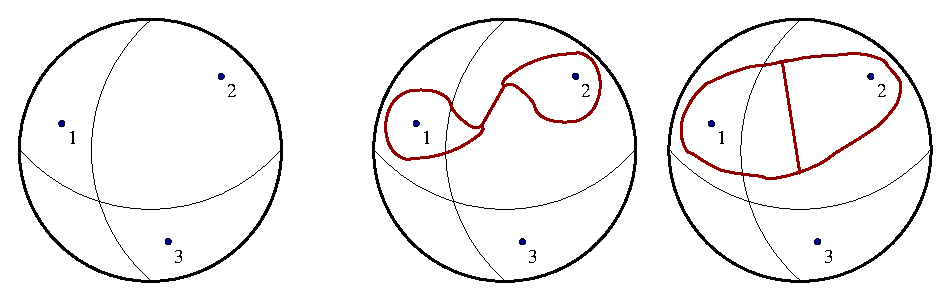
\includegraphics[width=\textwidth]{sfera3}
  \caption{A thrice-punctured sphere and two deformation retracts, not
    isomorphic as graphs.}
  \label{fig:sphere-retracts}
\end{figure}
We can refine this correspondence by introducing more structure on the
graph.
\begin{definition}
  \label{dfn:metric-ribbon-graphs}
  A metrized ribbon graph $(G, \ell)$ is a ribbon graph $G$ equipped with
  a real positive number $\ell_\alpha$ for each edge $\alpha \in \Edges{G}$.
\end{definition}

We can give the topological Riemann surface $S(G)$ a complex
structure by means of a triangulation and an analytic atlas.

In the course of the construction of $S(G)$, two punctured disk have
been glued on the sides of an edge $\alpha \in \Edges{G}$: call them $\alpha^+$
and $\alpha^-$; they are not necessarily distinct.  Let $T_\alpha^+$ and $T_\alpha^-$
be the triangles delimited by $\alpha$ and the radii joining endpoints of
$\alpha$ with the puncture of $\alpha^\pm$. The collection $\{T_\alpha^\pm : \alpha \in
\Edges{G}\}$ is a triangulation of $S(G)$.

Define an atlas of $S(G)$:
\begin{itemize}
\item for any edge $\alpha \in \Edges{G}$, put $V_\alpha := (T_\alpha^+ \cup T_\alpha^-)^\circ$;
\item for any boundary component $\beta \in \Holes{G}$, put $V_\beta := \bigl(
  \bigcup_{\alpha} T_\alpha \bigr)^\circ$ for all $\alpha$ bounding $\beta$;
\item for any vertex $\gamma \in \Vertices{G}$, put $V_\gamma := \bigl( \bigcup_\alpha T_a^\pm
  \bigr)^\circ$ for all $\alpha$ incident to $\gamma$.
\end{itemize}
\begin{figure}[btp]
  %% Figura atlas.fig
  \centering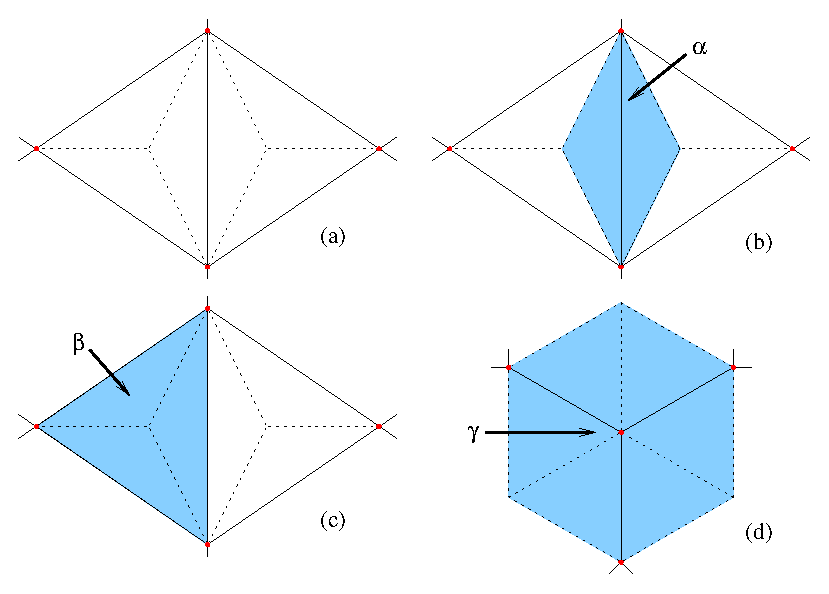
\includegraphics[width=\textwidth]{atlas}
  \caption{The open sets building an atlas of $S(G)$: (a) the
    triangulation built from a graph $G$: graph edges are drawn as
    solid lines, and edges of $T_\alpha^{\pm}$ are drawn as dotted lines; (b)
    the neighborhood $V_\alpha$ of an edge $\alpha$; (c) the neighborhood $V_\beta$
    of a boundary component $\beta$; (d) the neighborhood $V_\gamma$ of a
    vertex $\gamma$.}
  \label{fig:atlas}
\end{figure}

Define charts on the open sets $V_*$ (see Figure~\ref{fig:charts}):
\begin{itemize}
\item for any edge $\alpha$, pick a homeomorphism $f_\alpha: V_\alpha \to \{ z \in \setC
  : 0 < \Re z < \ell_\alpha \}$;
\item for any boundary component $\beta$, bounded by edges $\alpha_1$, $\alpha_2$
  and $\alpha_3$, pick a homeomorphism $f_\beta: V_\beta \to \{ \abs{z} < \rho \}$, where
  $\rho = (\ell_{\alpha_1} + \ell_{\alpha_2} + \ell_{\alpha_3}) / 2\pi$.
\item for any vertex $\gamma$, pick a homeomorphism $f_\gamma: V_\gamma \to \setC$.
\end{itemize}
\begin{figure}[htbp]
  %% Figura charts.fig
  \centering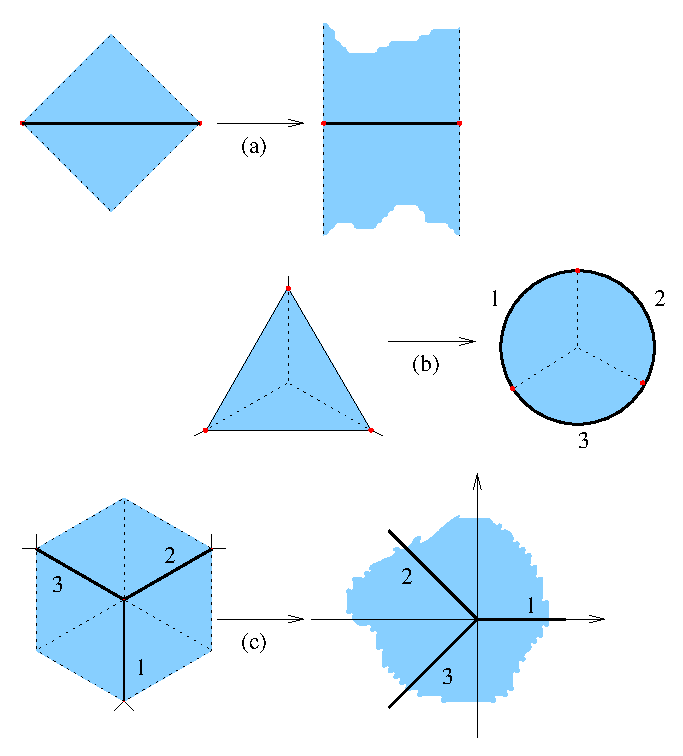
\includegraphics{charts}
  \caption{Local charts on the atlas: (a) any open set $V_\alpha$
    maps to a strip in the complex plane; (b) any open set $V_\beta$
    maps to a disk; (c) any open set $V_\gamma$ maps to the complex
    plane itself.}
  \label{fig:charts}
\end{figure}
These choices are subject to the condition that transition functions
satisfy the following:
\begin{itemize}
\item if $\alpha$ is an edge bounding the hole $\beta$, then $f_\beta \circ
  f_\alpha^{-1} = \exp (2\pi\I z / p_\beta)$ with $p_\beta := \sum_{\alpha \in \beta} \ell_\alpha$
  (\emph{perimeter} of the hole $\beta$);
\item if $\alpha$ is incident to a vertex $\gamma$, then $f_\gamma \circ f_\alpha^{-1} =
  c \cdot z^{2/(v+2)}$, up to a complex constant of modulus $1$, where
  $v$ is the valence of the vertex $\gamma$.
\end{itemize}

In the end, we have come upon a complex analytic structure on $S(G)$,
which depends on the perimeters $p_1, \ldots, p_n$ of boundary components
$\beta_1, \ldots, \beta_n$. By varying these (real positive) parameters, one can
vary the complex structure on $S(G)$; this will allow for a different
construction of the moduli space $\M_{g,n}$.

The perimeters $p_1$, \ldots, $p_n$ depend on the matric data $\ell_\alpha$,
therefore the complex analytic structure on $S(G)$ actually depends on
the metrized graph $(G, \ell)$.  Let $S(G, \ell)$ denote the Riemann
surface $S(G)$ endowed with this complex analytic structure.

\begin{remark}
  Note that the above procedure actually equips any metrized ribbon
  graph $(G, \ell)$ with a structure of embeddded ribbon graph: take the
  obvious $\iota:G \to S(G, \ell)$ as immersion of the graph, and maps $f_\beta$ as
  the homeorphisms between $S \setminus \iota(G)$ and punctured disks.
\end{remark}


\subsection{Construction of $\Tcomb_{g,n}$ and $\Mcomb_{g,n}$}
\label{sec:mgn-comb-construction}

Let $G$ be a metrized ribbon graph of genus $g$ with $n$ numbered
boundary components.  A topological cell $\Delta(G) \subseteq \M_{g,n}$ is spanned
when varying the metric data $(\ell_\alpha)_{\alpha \in \Edges{G}}$; gluing these
cells one recovers the whole $\M_{g,n}$.  A construction of
$\Tcomb_{g,n}$ can be found in \cite{penner:math.GT/0210326}, although
the actual procedure mimicks
\cite{kontsevich;intersection-theory;1992}.

Call a set $X \subseteq \Edges{G}$ negligible whenever it is \emph{not} the
support of a non-trivial homological cycle.  For an abstract ribbon
graph $G$, define:
\begin{equation*}
  \label{eq:rg-cells-moduli}
  \Delta(G) := \{ \ell: \Edges{G} \to \setR_{\geq0} | \text{the zero set of $\ell$ is negligible}\}.
\end{equation*}
It is a contravariant functor from the category of abstract ribbon
graphs to the category of topological spaces: if $G'$ is obtained from
$G$ by contracting the edge $\alpha$, then
\begin{equation}\label{eq:embedding-cells}
  \Delta(G') = \{ \ell \in \Delta(G) | \ell_\alpha = 0 \}.
\end{equation}
By composing with the forgetful functor $[G, \iota, \psi_*] \mapsto G$ from
embedded ribbon graphs to abstract ribbon graphs, we define a
contravariant functor on the category of embedded ribbon graphs:
\begin{equation*}
  \label{eq:rg-cells-teichmueller}
  T\Delta[G, \iota, \psi_*] := \Delta(G).
\end{equation*}

\begin{definition}
  The combinatorial Teichm\"uller space is the direct limit of the
  functor $T\Delta$:\FIXME{%
    In realt\`a, Penner costruisce questo spazio non come limite
    diretto, ma incollando esplicitamente le celle.  C'\`e qualcosa di
    nascosto che non funziona col limite diretto?  Per esempio si fa a
    meno del lemma~\ref{lemma:erg-no-aut}.  }%
  \begin{equation*}
    \Tcomb_{g,n} := \varinjlim T\Delta[G, \iota, \psi_*],
  \end{equation*}
  where $[G, \iota, \psi_*]$ ranges in the category $\ERG{g,n}$ of embedded
  ribbon graphs of genus $g$ with $n$ numbered boundary components.
\end{definition}
$\Tcomb_{g,n}$ is obtained by gluing topological cells $\Delta(G)$ alongside
the boundary: if $[G', \iota', \psi'_*]$ is obtained from $[G, \iota, \psi_*]$ by
contraction of an edge $\alpha$, then $\Delta(G')$ is identified with the face
of $\Delta(G)$ where $\ell_\alpha = 0$ by \csref{eq:embedding-cells}.

Elements of the topological space $\Tcomb_{g,n}$ are (equivalence
classes of) metrized embedded ribbon graphs $[G, \iota, \psi_*, \ell]$, where $\ell
\in T\Delta[G, \iota, \psi_*]$; it is easy to check that any $[G, \iota, \psi_*, \ell] \in
\Tcomb_{g,n}$ has a unique representative such that $\ell_\alpha > 0$ for all
$\alpha \in \Edges{G}$.  Perimeter maps $p_\beta: \Tcomb_{g,n} \to \setR_{>0}$ are
well-defined; write $p_j$ for the perimeter of the $j$-th hole.

\begin{definition}
  The combinatorial moduli space of curves is the direct limit of the
  functor $\Delta$:
  \begin{equation*}
    \Mcomb_{g,n} := \varinjlim \Delta(G),
  \end{equation*}
  where $G$ ranges in the category $\RG{g,n}$ of abstract ribbon
  graphs of genus $g$ with $n$ numbered boundary components.
\end{definition}

The functorial action of $\Gamma_{g,n}$ on $\ERG{g,n}$ induces an action
on $\Tcomb_{g,n}$.
\begin{lemma}
  \label{lemma:penner-kontsevich-bridge}
  $\Mcomb_{g,n}$ is the quotient space (in the orbifold sense) of
  $\Tcomb_{g,n}$ by the action of the mapping class group $\Gamma_{g,n}$.
\end{lemma}
\begin{proof}
  If $G \in \RG{g,n}$ is any abstract ribbon graph, then map $\Delta(G)$ into
  $\Tcomb_{g,n} / \Gamma_{g,n}$ by the following: pick any representative
  embedding ${\tilde G} = [G, \iota, \psi_*] \in \ERG{g,n}$ of $G$ and compose
  the isomorphism $\Delta(G) \cong T\Delta(\tilde G)$ with the quotient
  projection $T\Delta(\tilde G) \to \Tcomb_{g,n}/\Gamma_{g,n}$.  The mapping
  is well-defined: if $[G, \iota, \psi_*]$ and $[G, \iota', \psi'_*]$ are two
  distinct embeddedings of $G$, then ${\tilde \iota}, {\tilde \iota'}: S(G) \to
  S$ are homemorphisms, and, for any $\ell \in \Delta(G)$, $\iota' \circ \iota^{-1}$ is
  differentiable with respect to the analytic structure $S(G, \ell)$.
  Therefore, if $\phi := (\iota')^{-1} \circ \iota$, then $[G, \iota, \psi_*] = \phi \cdot [G, \iota',
  \psi'_*]$.

  By definition of direct limit, a map $\Phi$ is induced $\Mcomb_{g,n} \to
  \Tcomb_{g,n} / \Gamma_{g,n}$.  It is surjective: every point in $\Tcomb /
  \Gamma$ is a projection of a point $[G, \iota, \psi_*] \in \Tcomb$, therefore it
  is in the image of $G \in \Mcomb$.  $\Phi$ is injective: if $G$ and $G'$
  map to the same point in $\Tcomb / \Gamma$, then there is some $\phi \in \Gamma$
  such that $[G, \iota, \psi_*] = \phi \cdot [G', \iota', \psi'_*] = [G', \phi \circ \iota, \psi'_* \circ
  \phi]$; therefore, there is $\phi' \in \Diff^0$ such that $\phi' \circ \iota = \phi \circ \iota'$.
  Thus $f = \iota' \circ \iota^{-1}: G' \to G$ is a isomorphism of ribbon
  graphs.\FIXME{Questa ``dimostrazione'' non mi convince molto.}
\end{proof}

As in the final part of the proof of
\csref{lemma:penner-kontsevich-bridge}, we can see that the image
$M(G) \subseteq \Mcomb$ of a cell $\Delta(G)$ is the quotient of $\Delta(G)$ by $\Aut
G$.  The orbicells $M(G)$ are glued alongside the boundary, according
to the same procedure as in $\Tcomb$: if $G'$ is a contraction of $G$,
then $M(G')$ is a face of $M(G)$). Therefore, $\Mcomb_{g,n}$ is a
orbifold.

The cell $M(G)$ has real dimension $\card{\Edges{G}}$; therefore,
cells of maximal dimension are given by graphs with all vertices of
valence $3$. The union of these cells is a dense subset of
$\Mcomb_{g,n}$ with non-void interior.

\subsubsection{Kontsevich' compactification of $\Mcomb_{g,n}$}
\label{sec:comp-mcomb}
The construction of $\Mcomb_{g,n}$ can be done with slightly changed
rules: if we define a set $X \subseteq \Edges{G}$ to be negligible iff it does
not contain \emph{all} edges bounding a hole, then we can define a
contrafunctor $\overline{M}(G)$ and a topological space:
\begin{equation*}
  \label{eq:kontsevich-4}
  \Mbarcomb_{g,n} := \varinjlim \overline{M}(G).
\end{equation*}
$\Mbarcomb_{g,n}$ turns out to be a compactification of the orbifold
$\Mcomb_{g,n}$. 


\subsection{From surfaces to graphs: the Jenkins-Strebel Theorem}
\label{sec:strebel}
A theorem proved independently by J.~A. Jenkins \cite{jenkins;annals}
and K.~Strebel \cite{strebel;quadratic-differentials;1983} provides
the key tool for the inverse route: the construction of ribbon graphs
from smooth complex curves.

\begin{definition}
  A quadratic differential $q$ on a Riemann surface $S$ is a
  (meromorphic) section of $(T^*S)\tp2$.
\end{definition}
The set of vectors in $T_zS$ on which $q$ takes real non-negative
values forms a real line in $T_zS$: therefore, they make up a
foliation $F = F_qS$ on $S \setminus \{\text{poles of $q$}\}$. The non-compact
leaves of $F$ together with zeroes of $q$ form the ``critical locus''
of $q$.  

The set of vectors in $T_zS$ on which $q$ takes a purely imaginary
value form a perpendicular foliation $F^\perp$, whose leaves connect
either two distinct poles $x_i$ and $x_j$, or a pole $x_i$ and a zero
$v_j$.

Every quadratic differential $q$ induces a metric (away from the
critical locus) by $\ud s^2 = \abs{q(z)} \cdot \abs{\ud z}$.

\begin{theorem}[Jenkins, Strebel; {\cite[Theorem 23.2 and
    23.5]{strebel;quadratic-differentials;1983}}] 
  \label{thm:JS}
  For any complex analytic curve $S$ with $n$ marked points $x_1, \ldots,
  x_n$, and any assignment of real positive numbers $p_1, \ldots, p_n$,
  there exists one and only one quadratic differential $q$ such that:
  \begin{itemize}
  \item the only poles of $q$ occur at the marked points $x_1, \ldots, x_n$
    with second residue $p_1, ..., p_n$, that is, in a local
    coordinate $z_i$ near $x_i$ we have:
    \begin{equation*}
      q = -p_i^2 (\d z_i^2 / z_i^2) + \text{higher order terms};
    \end{equation*}
  \item the non-critical real trajectories of $F_q$ are simple closed
    circles around $x_i$.
  \end{itemize}
  Furthermore, $q$ has the following properties:
  \begin{itemize}
  \item every nonsingular closed leaf circling around $x_i$ has length
    $p_i$ in the flat metric induced by $q$.
  \item the critical locus of $q$ is a graph $G$ embedded in $S$;
  \item the complement $S \setminus G$ of the critical locus is a collection
    of disks $\{D_i | i=1,\ldots,n\}$, each one centered at a pole $x_i$, and
    the projective class of the collection of radii of disks $\{D_i\}$
    equals the projective class $[p_1, \ldots, p_n]$.
  \end{itemize}
\end{theorem}
The critical graph $G$ inherits a structure of embedded ribbon graph
with metric from the ambient surface $S$: the length of an edge $\alpha$ is
the one measured in the metric induced by the quadratic differential.
Furthermore, Jenkins-Strebel's theory states that $G$ has a vertex of
valence $k+2$ where $q$ has a zero of order $k$, therefore, vertices
of $G$ have valence $\geq3$. 

Since the markings $x_1, \ldots, x_n$ are \emph{ordered}, $G$ has an
additional structure of \emph{numbered} graph, that is, it is endowed
with a bijection $h: \Holes{G} \to \{1, \ldots, n\}$.


\subsection{Relation with $\M_{g,n}$ and $\T_{g,n}$}
\label{sec:nocomb}

\begin{theorem}[Harer, Mumford, Thurston;
  \cite{harer;cohomological-dimension,
    looijenga;cellular-decomposition, penner:math.GT/0210326}] 
  The Jenkins-Strebel construction defines morphisms
  \begin{equation*}
    \T_{g,n} \times \setR_{>0}^n \to \Tcomb_{g,n}, 
    \qquad
    \M_{g,n} \times \setR_{>0}^n \to \Mcomb_{g,n}, 
    \qquad 
    \Mbar_{g,n} \times \setR_{>0}^n \to \Mbarcomb_{g,n}.
  \end{equation*}
  The first of these is a homeomorphism and the second is an orbifold
  equivalence. 

  The inverse map
  \begin{equation*}
    \Tcomb_{g,n} \to \T_{g,n} \times \setR_{>0}^n \to \setR_{>0}^n,
    \qquad
    \Mcomb_{g,n} \to \M_{g,n} \times \setR_{>0}^n \to \setR_{>0}^n
  \end{equation*}
  is the perimeter map $\pi := (p_1, \ldots, p_n)$.  
\end{theorem}

For any given $p^\circ = (p_1^\circ, \ldots, p_n^\circ) \in \setR_{>0}^n$, the fiber
$\pi^{-1}(p^\circ)$ is isomorphic to $\M_{g,n}$ (resp.\ $\T_{g,n}$), thus,
$\pi$ induces a triangulation of $\M_{g,n}$ (resp.\ $\T_{g,n}$).



\section{Harer's equivariant spine for Teichm\"uller space}
\label{sec:spine}

Harer \cite{harer;cohomological-dimension}, introduced a simplicial
spine for the Teichm\"uller space $\T_{g,n}$.  

If $X$ is any semi-simplicial complex, denote by $X'$ its first
barycentric subdivision, and by $|X|$ its geometric realization.


\subsection{Arc-systems}
\label{sec:arc-systems}

Let $T_{g,n}$ be a topological compact oriented Riemann surface of
fixed genus $g$ with $n$ marked points $x_1, \ldots, x_n$.  Regard points
in the moduli space $\M_{g,n}$ as equivalence classes $(S,x,\varphi)$ of a
complex analytic curve $S$ with a marking $x:\{1,\ldots,n\}\to S$ and a
homeomorphism $\varphi:S\to T_{g,n}$ with the reference surface (see
\csref{sec:alternate-Mgn}).

If $u$ is any arc in $S$, denote by $[u]$ its isotopy class rel~$\{x_1,
\ldots, x_n\}$.
\begin{definition}
  An arc-system $[u_1, \ldots, u_k]$ of rank $k$ is an isotopy class
  rel~$\{x_1, \ldots, x_n\}$ of $k$ properly imbedded arcs $u_i : [0,1] \to S$
  such that:
  \begin{itemize}
  \item every $u_i$ has its endpoints in the set $\{x_1, \ldots, x_n\}$;
  \item if $i \neq j$, then $u_i$ meet $u_j$ only at endpoints, if at all;
  \item no $u_i$ is null-homotopic rel~$\{x_1, \ldots, x_n\}$;
  \item no $u_i$ is homotopic rel~$\{x_1, \ldots, x_n\}$ to $u_j$, for $i \neq
    j$;
  \end{itemize}
  An arc-system $[u_1, \ldots, u_k]$ is said to \emph{fill up} the curve
  $S$ iff all connected components of $S - \bigcup\{u_i\} - \{x_1,\ldots x_n\}$ are
  either disks or punctured disks.
\end{definition}

Arc-systems may be organized into a semi-simplicial complex.
\begin{definition}
  $\U$ is the semi-simplicial complex having a simplex $\langle u_1, \ldots, u_k\rangle$
  for every rank $k$ arc-system $[u_1, \ldots u_k]$, with the proviso that
  $\langle u'_1, \ldots, u'_l\rangle$ is a face of $\langle u_1, \ldots, u_k\rangle$ iff $\{ [u'_1], \ldots,
  [u'_l] \} \subset \{ [u_1], \ldots, [u_k] \}$.
  
  $\U_0$ is the subcomplex of all those simplices $\langle u_1, \ldots, u_k\rangle$
  that do not fill up the surface $S$.
\end{definition}

Let $U'$, $U_0'$ be the first barycentric subdivisions of $U$
and $U_0$, respectively.

\begin{definition}
  Let $Y'$ be the collection of simplices in $U'$ having no face in
  $U_0'$; equivalently, $\sigma_\bullet \in Y'$ iff every vertex of $\sigma_\bullet$
  lies in $U' \setminus U_0'$.
\end{definition}
$Y'$ is a full subcomplex of $U'$.

There is a natural action of $\Gamma_{g,n}$ on $U$ given by $g \cdot [u_1, \ldots
u_k] = [g \circ u_1, \ldots, g \circ u_k]$; it preserves $U_0$, so it restricts to
an action on $U \setminus U_0$.

Let $\Delta^{n-1}$ be the $(n-1)$-dimensional geometric simplex.
\begin{theorem}[Harer, {\cite[Theorem
  1.3]{harer;cohomological-dimension}}]
There exists a $\Gamma_{g,n}$-equivariant homeomorphism $\Phi: \T_{g,n} \times
\Delta^{n-1} \to |X \setminus X_0|$.
\end{theorem}
This is another consequence of \ref{thm:JS}


%%% Local Variables: 
%%% mode: latex
%%% TeX-master: "index"
%%% x-symbol-8bits: nil
%%% End: 


\chapter{An algorithm for computing graph homology}
\label{chap:algorithm}

This chapter presents an algorithm to compute homology of the fatgraph
complex $\R_{g,n}$.  By \csref{thm:fatgraph-homology}, this is
tantamount to the (co)homology with rational coefficients of the
moduli spaces $\M_{g,n}$. An effective computer implementation of the
algorithm is presented, which is capable of computing the Betti
numbers of $\M_{g,n}$ for $(2g+n) < 6$ on standard desktop-class
hardware.  The size of the fatgraph complex increases factorially with
$2g+n$, so a parallel algorithm is needed to compute the Betti numbers
of $\M_{g,n}$ for $(2g+n) \geq 6$; this will be the subject of a later
chapter.

Generators of the homology modules could be computed with a little
variant in the last step of the algorithm; however, this is not
interesting in connection with the homology of $\M_{g,n}$, since
expression of a fatgraph homology class in terms of algebro-geometric
classes has proved to be a difficult problem 
\cite{mondello:2004,
  igusa:combinatorial-miller-morita-mumford-classes-and-witten-cycles,
  igusa:graph-cohomology-and-kontsevich-cycles},
and to-date lacks a general solution.

The Python programming language is used in this chapter to articulate
the algorithm.  Python claims to be ``executable pseudo-code'',
combining a readable and ``natural'' syntax that makes it well suited
to teaching programming to novices \cite{georgatos:python}, with the
power of a general-purpose language that is presently in daily use for
several real-world applications (see, e.g., \cite{python:success}).
The advantage is clear: the code listed in this chapter can be copied
to a Python file and actually executed.  For the reader's convenience,
\csref{chap:python} recaps the Python syntax and briefly explains the
constructs and idioms used in programming this algorithm.


\section[Overview]{Overview of the algorithm}
\label{sec:overview}

\csref{thm:fatgraph-homology} provides an effective way to compute the
(co)homology of $\M_{g,n}$.  The Betti numbers of $\M_{g,n}$ can be
computed from the knowledge of the dimension of chain spaces $W_p$ and
the ranks of the boundary operators $D_p$; this can effectively be
accomplished in the following stages:
\begin{enumerate}[I.]
\item Compute the basis set of $W_*$; by definition, the basis set is
  the set of \emph{orientable} fatgraphs indexing
  the cells of $\Mcomb_{g,n}$.
\item Work out the differential $D: W_* \to W_*$ in an
  effectively computable way, i.e., as matrix operators $D_p$ mapping
  coordinates in the fatgraph basis of $W_p$ into coordinates
  w.r.t. the fatgraph basis of $W_{p-1}$.
\item Compute the ranks of the matrices $D_p$.
\end{enumerate}

Stage~I needs just the pair $g,n$ as input; its output is the set of
orientable numbered fatgraphs belonging in $\R_{g,n}$: the core of
Stage~I is an algorithm to enumerate the fatgraph of given genus and
number of boundary cycles. By definition, numbered fatgraphs are
decorated abstract fatgraphs, and the decoration is a simple
combinatorial datum: therefore, the problem can be reduced to
enumerating abstract fatgraphs.  With a recursive algorithm, one can
construct trivalent $\M_{g,n}$-fatgraphs from $\M_{g-1,n}$ and
$\M_{g',n'} \times \M_{g'',n''}$ with $g'+g''=g$ and $n'+n''=n$; all
other graphs are gotten by contraction of regular edges.

The differential $D$ has a simple geometrical definition: $D(G)$ is a
sum of graphs $G'$ gotten by contracting a non-loop edge of $G$. A
naive implementation of Stage~II would just compare each contraction
of a graph with $k$ edges with any graph with $k-1$ edges, and score a
$\pm 1$ in the corresponding entry of the matrix $D_k$.  However, this
algorithm has quadratic complexity, and the large number of graphs
involved make it very inefficient already for $\M_{0,5}$.  The simple
observation that contraction of edges is defined on the topological
fatgraph underlying a numbered fatgraph allows us to apply the naive
algorithm to topological fatgraphs ---which cuts complexity down by a
factor~$(n!)^2$---, and then extend the result by the action of graph
automorphism groups on the numberings of boundary cycles.  This
is the variant detailed in \csref{sec:stage-ii}.

Stage~III is the simplest: by elementary linear algebra, the Betti
numbers can be computed from the rank of matrices $D_k$ and the
dimension of their domain space.  The computational problem of
determining the rank of a matrix has been extensively studied, and
several implementations of popular algorithms are already available in
the form of function libraries, ready for use. It should be noted,
however, that this is the step that consumes more computer time
(except for the very simple cases $2g+n<5$).

\section[Stage I]{Stage I: generate the fatgraphs complex}
\label{sec:stage-i}

Exposition of the Stage~I code will proceed in a \emph{top-down}
fashion: we shall work our way from the topmost function, which
returns the collection of all fatgraphs in $\R_{g,n}$, down to the
computer representation of a fatgraph.  This way, requirements that
functions and objects must satisfy become evident during the analysis,
and implementation details are introduced only when needed.

\subsection{Generation of all Fatgraphs in $\R_{g,n}$}
\label{sec:stage1-all}

Computations in Stage~I output the set of orientable fatgraphs
$\R_{g,n}$ from the input pair $g, n$, with $2g +n - 2 > 0$.  The
numbering will be added in Stage~II of the algorithm, so just the set
of undecorated fatgraphs is output here.

Let \l{MgnGraphs} be the function which, given the two integers $g$,
$n$ as input, and returns the collection of $\R_{g,n}$ graphs.  Let us
further stipulate that the output result will be represented as a
Python \l{list}: the $0$-th item in this list is the list of graphs
with the maximal number $m$ of edges; the $k$-th item in the list is
the list of graphs having $m - k$ edges.  There are algorithmic
advantages in this subdivision, which are explained below.

The Python implementation of the \l{MgnGraphs} function is as follows:
\begin{lstlisting}[name=MgnGraphs,firstnumber=1]
def MgnGraphs(g,n):
  """
  Return all connected fatgraphs having
  prescribed genus `g` and number of boundary cycles `n`.
  """
  # `graphs` is the function output -- start with an empty list
  graphs = []

  # maximum number of edges
  m = 4*g + 2*n - 5
\end{lstlisting}
Graphs with the maximal number of edges are trivalent graphs; they are
computed by a separate function \l{MgnTrivalentGraphs}, described in
\csref{sec:stage1-trivalent}.
\begin{lstlisting}[name=MgnGraphs,firstnumber=11]
  # first item `graphs[0]` contains all 3-valent graphs
  graphs.append(list(MgnTrivalentGraphs(g,n)))
\end{lstlisting}
We can then proceed to generating all graphs in $\R_{g,n}$ by
sequential contraction of graphs edges: by contracting one edge in
trivalent graphs we get the list \l{graphs[1]} of all graphs with
$m-1$ edges; contracting one edge in $G \in \text{\l{graphs[1]}}$, we
get $F \in \text{\l{graphs[2]}}$ with $m-2$ edges; and so on:
\begin{lstlisting}[name=MgnGraphs,firstnumber=13]
  for k in range(1,m):
    graphs.append([]) # start with empty list
    for G in graphs[k-1]:
      for e in G.edge_orbits():
        if not e.is_loop():
          F = G.contract(e)
          if F not in graphs[k]:
            graphs[k].append(F)
\end{lstlisting}
A line-by-line explanation is in order:
\begin{itemize}
\item At line 13, the \l{range(1,m)} function sequentially generates
  all integers in the half-open range $[1, m)$; therefore, the
  \l{for}-loop body in lines 14--20 is executed $m-1$ times, with $k$
  taking the values $1$, ..., $m-1$ in order.  Note that, by Python
  syntax, the loop body is indented w.r.t the loop head line.
\item At line 14, \l{graph[k]} is initialized to an empty list:
  at the start of the loop body, the \l{graphs} list only has items
  \l{graphs[0]} through \l{graphs[k-1]}.
\item Line 15 introduces a new loop: code in lines 16--20 will be
  executed once for each fatgraph \l{G} in \l{graphs[k-1]}.
\item Line 16 starts the core of the function: contract edges of
  the fatgraph \l{G} to generate new fatgraphs with $m-k$ edges.
  However, we need not contract every edge of a fatgraph: if $a \in
  \Aut(G)$ is an automorphism and $x \in E(G)$ is an edge, then the
  contracted graphs $G' = G/x$ and $G'' = G/a(x)$ are isomorphic.
  Hence, we can restrict the computation to consider only one edge per
  orbit of the action induced by $\Aut(G)$ on the set $E(G)$. This is
  what the method call \l{G.edge_orbits()} provides: for each graph
  \l{G}, it partitions the set of edges of \l{G} into orbits and
  returns one representative edge \l{e} for each one.
\item Line 17 skips non-regular edges: the following code is executed
  if and only if \l{e} is not a loop.
\item Line 18 computes the fatgraph \l{F} obtained by contracting the
  current edge \l{e} in \l{G}: the \l{Fatgraph.contract(G,e)} invocation
  returns a \emph{new} fatgraph instance obtained by applying
  topological contraction.
\item Lines 19--20 add \l{F} to \l{graphs[k]} \emph{only if it is not
    already there}.  This is actually very concise syntax for the most
  computationally expensive part of the \l{MgnGraphs} function: Python
  performs a comparison between \l{F} and each element in
  \l{graphs[k]}; each comparison invokes the \l{Fatgraph.__eq__}
  method, which in turn invokes \l{Fatgraph.isomorphism}.  

  If $L = \text{\l{len(graph[k])}}$ is the number of elements in
  \l{graph[k]} and $T_\text{iso}$ is the average time needed to
  determine if two graphs are isomorphic, evaluating the expression
  \l{F in graphs[k]} takes $O(L \cdot T_\text{iso})$ time: thus, the
  subdivision of \l{graphs} into lists, each one holding graphs with a
  specific number of edges, reduces the number of fatgraph comparisons
  done in the innermost loop of \l{MgnGraphs}.  (Although graphs with
  a different number of edges are readily seen not to be isomorphic,
  since the test is performed in the innermost loop, it is executed
  nonetheless a considerable number of times, and each saving, albeit
  small, can result in a substantial shortening of the total running
  time.)
\end{itemize}

Finally, function \l{MgnGraphs} exits and returns the list \l{graphs} to the
caller:
\begin{lstlisting}[name=MgnGraphs,firstnumber=21]
  # `graphs` is the final output of this function
  return graphs
\end{lstlisting}

Note that the top-level function \l{MgnGraphs} is quite independent of
the actual Python implementation of the \l{Fatgraph} type of objects:
all is needed here, is that a \l{Fatgraph} instance has methods for
enumerating edges, contract an edge, and test two graphs for equality.


\subsection{Generation of Trivalent Fatgraphs}
\label{sec:stage1-trivalent}

\begin{lstlisting}
def MgnTrivalentGraphs(g, n):
  """
  Return a list of all connected trivalent fatgraphs having the
  prescribed genus `g` and number of boundary cycles `n`.
  """
  # avoid infinite recursion in later statements
  if n==0 or (g,n)<(0,3):
    raise StopIteration

  # $M_{0,3}$ --- induction base
  if (g,n) == (0,3):
    yield Fatgraph([Vertex([1, 2, 1]), Vertex([2, 0, 0])])
    yield Fatgraph([Vertex([1, 0, 2]), Vertex([2, 0, 1])])

  # $M_{1,1}$ --- induction base
  elif (g,n) == (1,1):
    yield Fatgraph([Vertex([1, 0, 2]), Vertex([2, 1, 0])])

  # general case
  else:
    def graphs(g,n):
      # pass 1: hang a circle to all edges of graphs in $M_{g,n-1}$
      for G in MgnTrivalentGraphs(g,n-1):
        for x in G.edge_orbits():
          yield G.hangcircle(x,0)
          yield G.hangcircle(x,1)

      # pass 2: bridge all edges of a single graph in $M_{g,n-1}$
      for G in MgnTrivalentGraphs(g,n-1):
        for (x,y) in G.edge_pair_orbits():
          yield G.bridge(x,0, y,0)
          yield G.bridge(x,0, y,1)
          yield G.bridge(x,1, y,0)
          yield G.bridge(x,1, y,1)

      # pass 3: bridge all edges of a single graph in $M_{g-1,n+1}$
      for G in MgnTrivalentGraphs(g-1,n+1):
        for (x,y) in G.edge_pair_orbits():
          yield G.bridge(x,0, y,0)
          yield G.bridge(x,0, y,1)
          yield G.bridge(x,1, y,0)
          yield G.bridge(x,1, y,1)

    unique = []
    for G in graphs(g,n):
      if (G.genus, G.num_boundary_cycles) == (g,n) \
          and (G not in unique):
        unique.append(G)
        yield G
\end{lstlisting}


\subsection{Computer representation of Fatgraphs}
\label{sec:stage1-fatgraphs}



\section[Stage II]{Stage II: compute boundary operator matrices}
\label{sec:stage-ii}

\section[Stage III]{Stage III: compute Betti numbers of $\M_{g,n}$}
\label{sec:stage-iii}



%%% Local Variables: 
%%% mode: latex
%%% TeX-master: "index"
%%% End: 

\RCSID $Id: gc.tex,v 1.5 2006/05/13 16:34:34 rmurri Exp $
%auto-ignore


\chapter{The Graphical Formalism for Symmetric Tensor Categories}
\label{cha:gc}

The graphical formalism for braided tensor categories was developed in
the late 1980's, when a categorical formulation of polynomial knot
invariants was given \cite{freyd-yetter;btc, turaev;yang-baxter}.
After this discovery, braided tensor categories were recognized as a
``reasonably general setting'' \cite{joyal-street;tensor-calculus}
where the graphical notation for tensors ---which, infact, dates back
to Penrose's \cite{penrose;negative-dimensional-tensors}--- could be
given firm grounds and a well-defined meaning.

This line of research culminated in
\cite{joyal-street;tensor-calculus} ---where it is shown how one can
parallely enrich the structure of a category and add more decorations
on the corresponding graphs--- and
\cite{reshetikhin-turaev;ribbon-graphs} ---where the final case of
autonomous tortile categories is settled.

I will not attempt here to give proofs of these results, but rather
derive the needed instances of graphical calculus as a
corollary to the most general results of Reshetikhin and Turaev.
However, proper statement of these requires quite a long preamble of
category-related material; I would therefore just skim over the
necessary definitions, and refer the interested reader to
\csref{cha:btc} and~\ref{cha:rt} for precise statements, and to the
foundational papers of Joyal and Street
\cite{joyal-street;tensor-calculus, joyal-street;btc} for details,
proofs, motivation and history.

As terminology in these matters is not yet generally agreed upon, I
will adhere to nomenclature used by Joyal and Street in
\cite{joyal-street;tensor-calculus, joyal-street;btc}. All relevant
definitions are grouped in \csref{cha:btc}.


\section{Graphical formalism for Symmetric Tensor Categories}
\label{sec:gc-stc}
\FIXME{In tutto questo capitolo, gli spazi di morfismi sono in verit{\`a}
  gli span lineari di quelli che sono veramente descritti\ldots}
Let $\A$ be a symmetric autonomous tortile category. For an object $A
\in \A$, let $A^{-1} := \rdl{A}$ and $A^{+1} := A$.
\begin{definition}\label{dfn:gc-graph-piece}
  An $\A$-colored elementary diagram piece is any one of the
  following:
  \begin{center}
    \begin{tabular}{cccccc}
      $\xy*!LC\xybox{(0,0)*+{A};(0,1)*+{A}**\dir{-}}\endxy$
      &
      $\xy*!LC\xybox{%
        \vcross~{(0,1)*+{B}}{(1,1)*+{A}}{(0,0)*+{A}}{(1,0)*+{B}}}\endxy$
      &
      $\xy*!LC\xybox{%
        \vcross~{(0,0)*+{B}}{(1,0)*+{A}}{(0,1)*+{A}}{(1,1)*+{B}}}\endxy$
      &
      $\xy*!LC\xybox{%
        \vloop~{(0,1)}{(1,1)}{(0,0)*+{A}}{(1,0)*+{A}}}\endxy$
      &
      $\xy*!LC\xybox{%
        \vloop~{(0,0)}{(1,0)}{(0,1)*+{A}}{(1,1)*+{A}}}\endxy$
      &
      $\xy*!LC\xybox{
        (0,1)*+[F]{f};%
        (-1,0)*+{A_1}**\dir{-},(-0.5,0)*+{A_2}**\dir{-},%
        (0,0.5)*+{\ldots},(1,0)*+{A_r}**\dir{-},%
        (-1,2)*+{B_1}**\dir{-},(-0.5,2)*+{B_2}**\dir{-},%
        (0,1.5)*+{\ldots},(1,2)*+{B_s}**\dir{-},%
        }\endxy$
      \\
      (a) & (b) & (c) & (d) & (e) & (f)
    \end{tabular}
  \end{center}
  For each strand $\ell$, some additional structure is specified:
  \begin{itemize}
  \item an object of $\A$;
  \item a sign $\varepsilon_\ell$, that is, an orientation;
  \item a framing, that is, a map $N_\ell: [0,1] \to S^1$ such that
    $N_\ell(0) = N_\ell(1) = 1$ (see \csref{sec:tortile} in
    \csref{cha:btc} for motivation).
  \end{itemize}
  
  Additionally, each piece of type (f) is decorated by a morphism $f
  \in \Hom\A$: if $\epsilon_1$, \ldots, $\epsilon_r$, $\eta_1$, \ldots, $\eta_s$ are the signs
  on the upper and lower strands of a piece of type (f), then $f \in
  \A(A_1^{\epsilon_1} \otimes \cdots \otimes A_r^{\epsilon_r}, B_1^{\eta_1} \otimes \cdots \otimes B_s^{\eta_s})$.
\end{definition}
A piece of type (a) is called a ``strand''; those of type (b) and (c)
are named ``crossings''; (d) and (e) are the ``coupling'' and the
``Casimir''; (f) is, plainly, a ``vertex''. The size of the rectangle
in a piece of type (f) is really immaterial.

We say the free strands at the bottom are ``input legs'' and those at
the top are ``output legs''. For a given piece $v$ of type (f), define
\begin{gather*}
  \Src(v) := A_1^{\epsilon_1} \otimes \cdots \otimes A_r^{\epsilon_r},
  \\
  \Tgt(v) := B_1^{\eta_1} \otimes \cdots \otimes B_r^{\eta_s},
\end{gather*}
if the $r$ input strands are decorated by objects $A_1$, \ldots, $A_r$ and
signs $\epsilon_1$, \ldots, $\epsilon_r$, while the $s$ output strands are decorated
by objects $B_1$, \ldots, $B_s$ and signs $\eta_1$, \ldots, $\eta_s$.

One can compose graph pieces $\Gamma_1$ and $\Gamma_2$ by stacking one on top
of the other (see \csref{fig:gc-graph-composition}), if $\Src(\Gamma_1) =
\Tgt(\Gamma_2)$, i.e., the input legs of $\Gamma_1$ match the output legs of
$\Gamma_2$ in number, color, orientation, and framing. The tensor product
of two graph pieces $\Gamma_1$ and $\Gamma_2$ is defined by juxtaposition, as
in \csref{fig:gc-graph-otimes}; note that no compatibility condition
is required in this case. We have the following:
\begin{align}
  \label{eq:src-comp-otimes}
  \Src(\Gamma_1 \circ \Gamma_2) &= \Src(\Gamma_2), 
  &&&
  \Src(\Gamma_1 \otimes \Gamma_2) &= \Src(\Gamma_1) \otimes \Src(\Gamma_2),
  \\
  \label{eq:tgt-comp-otimes}
  \Tgt(\Gamma_1 \circ \Gamma_2) &= \Tgt(\Gamma_1),
  &&&
  \Tgt(\Gamma_1 \otimes \Gamma_2) &= \Tgt(\Gamma_1) \otimes \Tgt(\Gamma_2).
\end{align}

We give the definition of the category of graphs in the arrows-only
form (see \csref{cha:arrows}). 
\begin{definition}
  The $\A$-colored \emph{diagrams} category $\RTD[\A]$ is the category
  whose morphisms are generated from $\A$-colored elementary pieces
  through the operations of graph composition and tensor product,
  defined as in figures~\ref{fig:gc-graph-composition}
  and~\ref{fig:gc-graph-otimes}.
  
  The $\A$-colored \emph{graph} category $\RTE[\A]$ is the category
  whose set of morphisms is the quotient of $\Hom\RTD[\A]$ by the
  Reidmeister-Reshetikhin-Turaev relations of \csref{fig:gc-rrt}.
\end{definition}
\begin{figure}[p]
  \centering\includegraphics{fig-001}
  \caption{Composition product of diagrams.}
  \label{fig:gc-graph-composition}
\end{figure}
\begin{figure}[p]
  \centering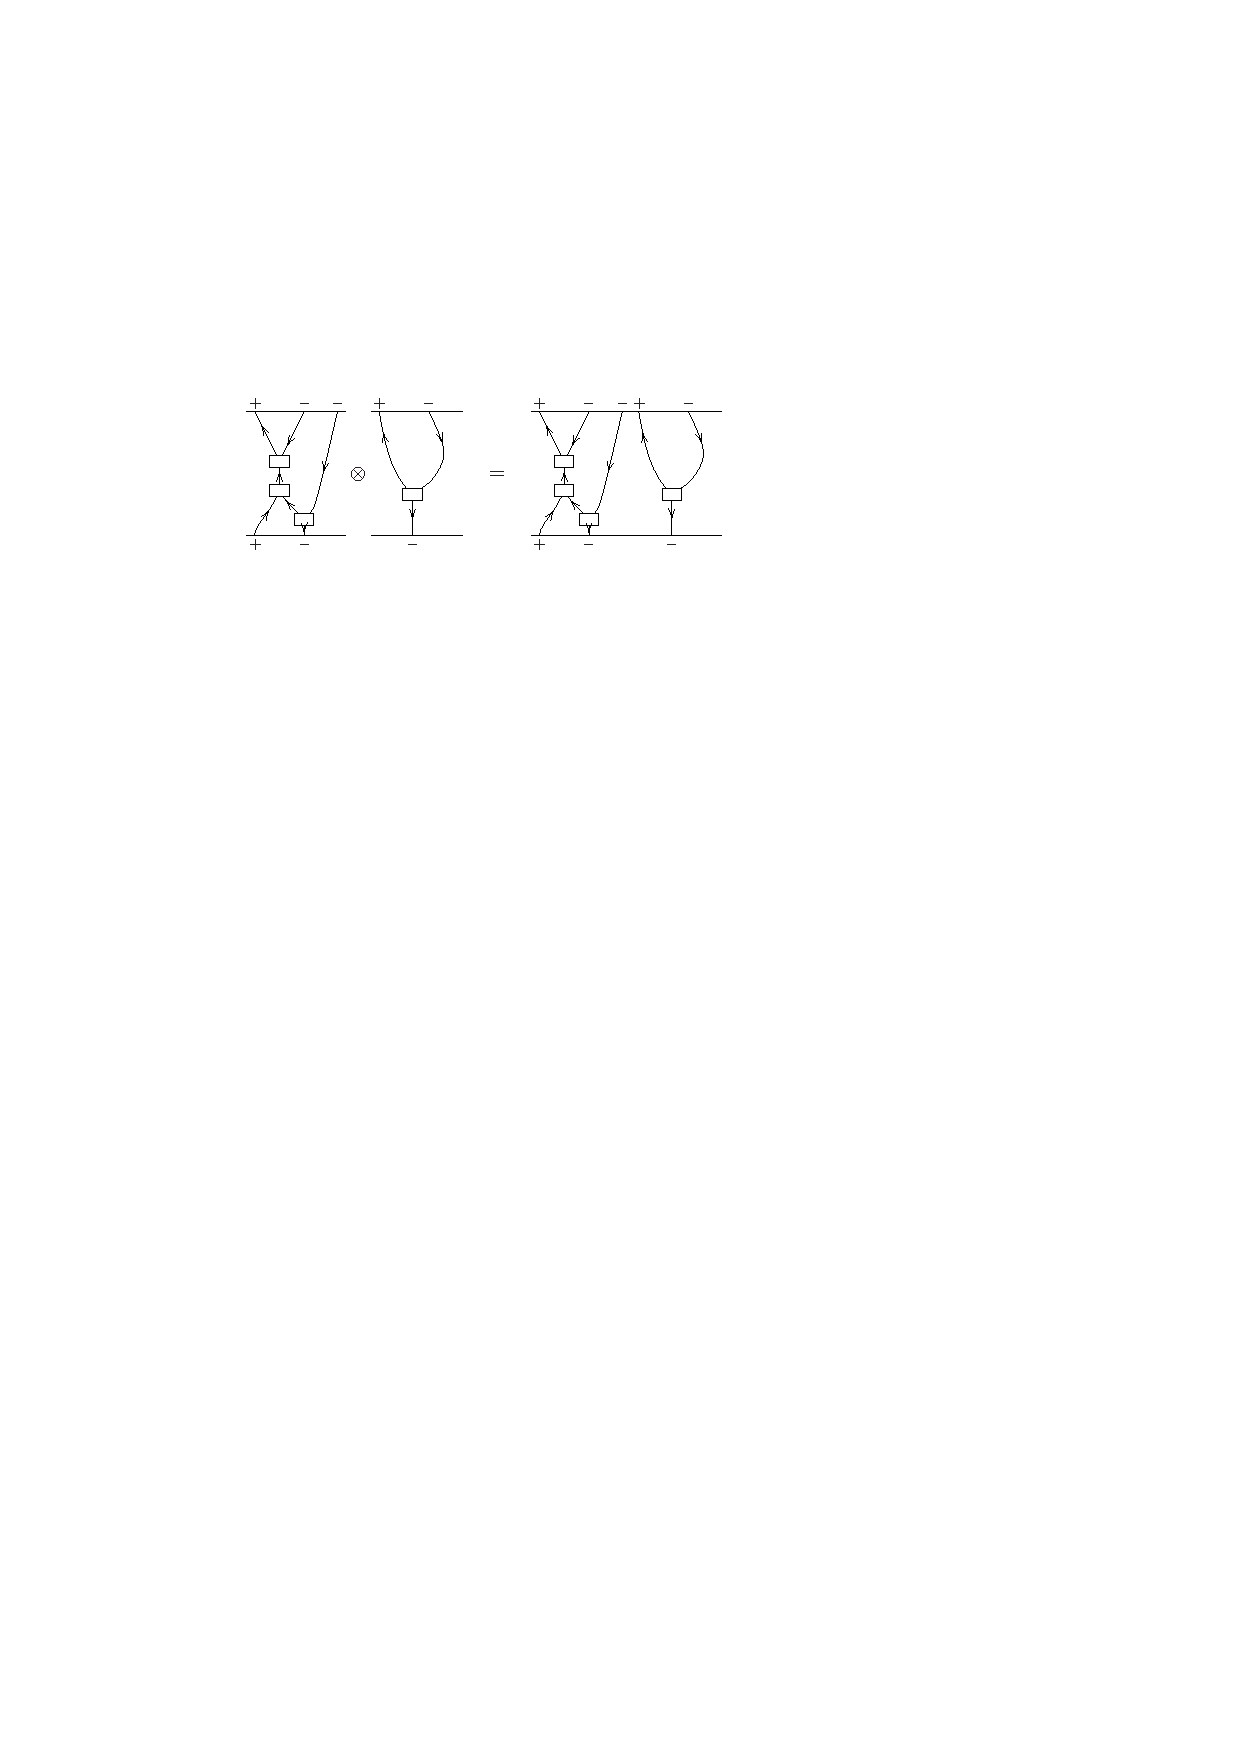
\includegraphics{fig-002}
  \caption{Tensor product of diagrams.}
  \label{fig:gc-graph-otimes}
\end{figure}
\begin{figure}[p]
  \centering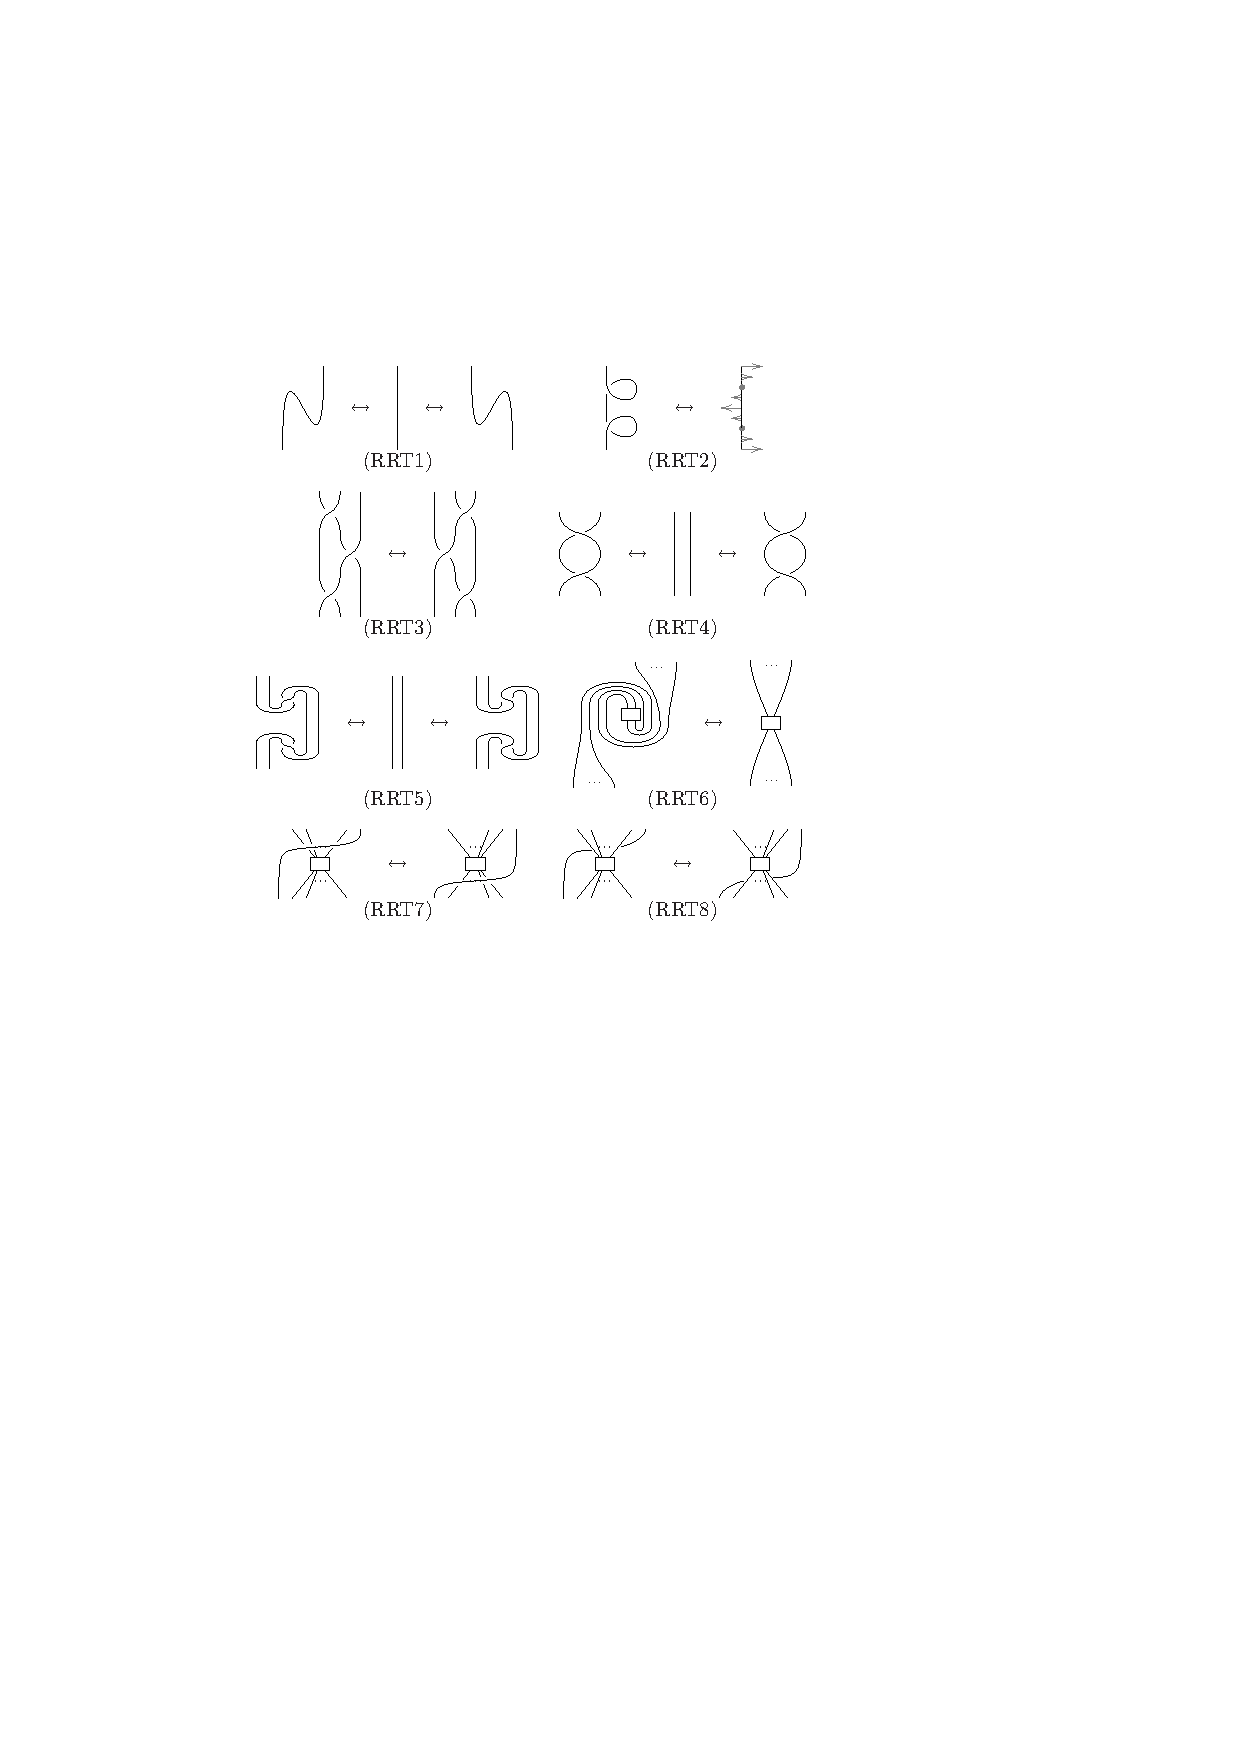
\includegraphics{fig-003}
  \caption{Reidmeister-Reshetikhin-Turaev moves for
    RT-diagrams. Note that (RRT2) changes a trivial framing
    into a non-trivial (degree $1$) one.}
  \label{fig:gc-rrt}
\end{figure}

Let $\category{B}$ be a tensor category. A tensor functor
$\RTD[\A]\to{\category{B}}$ is uniquely specified if we define it on the
generators; it induces a tensor functor $\RTE[\A] \to \category{B}$ if
it is compatible with relations (RRT1)--(RRT8) ---see
\csref{fig:gc-rrt}.  In particular, taking $\category{B}=\A$ we find
the following (see also \csref{thm:rt2} in \csref{cha:rt}).
\begin{theorem}[Reshetikhin-Turaev,
  \cite{reshetikhin-turaev;ribbon-graphs}]
  \label{thm:gc1}
  For any autonomous balanced braided tensor category $\A$, there is a
  tensor functor $Z_{\A}: \RTD[\A] \to \A$, mapping an object $(A_1,
  \ldots, A_r; \varepsilon_1, \ldots, \varepsilon_k) \in \RTD[\A]$ to $A_1^{\varepsilon_1} \otimes \dots \otimes
  A_k^{\varepsilon_k} \in \A$, and defined on generators of morphisms in
  $\RTD[\A]$ by
\begin{center}
  \everyxy={/r24pt/:}
  {%
    \begin{tabular}{ccc}
      $\xy*!LC\xybox{%
        \vcross~{(0,1)*+{B}}{(1,1)*+{A}}{(0,0)*+{A}}{(1,0)*+{B}}}\endxy
      \mapsto \tau_{XY},$
      %\label{graph-cross+}
      &
      $\xy*!LC\xybox{%
        \vcross~{(0,0)*+{B}}{(1,0)*+{A}}{(0,1)*+{A}}{(1,1)*+{B}}}\endxy
      \mapsto \tau_{XY}^{-1},$
      %\label{graph-cross-}
      &
      $\xy*!LC\xybox{
        (0,1)*+[F]{f};%
        (-1,0)*+{A_1}**\dir{-},(-0.5,0)*+{A_2}**\dir{-},%
        (0,0.5)*+{\ldots},(1,0)*+{A_r}**\dir{-},%
        (-1,2)*+{B_1}**\dir{-},(-0.5,2)*+{B_2}**\dir{-},%
        (0,1.5)*+{\ldots},(1,2)*+{B_s}**\dir{-},%
        }\endxy \mapsto f$
      %\label{graph-morphism} 
      \\
      $\xy*!LC\xybox{%
        \vloop~{(0,1)}{(1,1)}{(0,0)*+{A}}{(1,0)*+{A}}}\endxy \mapsto
      \ev_{A},$
      %\label{graph-casimir}
      &
      $\xy*!LC\xybox{%
        \vloop~{(0,0)}{(1,0)}{(0,1)*+{A}}{(1,1)*+{A}}}\endxy \mapsto
      \coev_{A},$
      %\label{graph-coupling}
      &
      $\xy*!LC\xybox{(0,0)*+{A};(0,1)*+{A}**\dir{-}}\endxy \mapsto
      \id_X,$
      %\label{graph-id}
    \end{tabular}
    }
  \end{center}
where $\tau_{AB}$, $\ev_A$, $\coev_A$ are the structure maps in
$\A$, and $f$ is a morphism in $\A$; take the dual of an
object if the sign $\varepsilon$ on the corresponding edge is $-1$.

The tensor functor $Z_\A$ is invariant by the
Reidmeister-Reshetikhin-Turaev moves (RRT1)--(RRT8), so it induces a
tortile braided functor $Z_\A: \RTE[\A] \to \A$.
\end{theorem}%
By definition of a symmetric category,
\begin{equation*}
  \tau_{AB} = \tau_{BA}\inv,
\end{equation*}
which imposes 
\begin{equation*}
  Z \left( 
    \xy*!LC\xybox{%
      \vcross~{(0,1)*+{B}}{(1,1)*+{A}}{(0,0)*+{A}}{(1,0)*+{B}}
      }\endxy \right)
  = 
  Z \left(
    \xy*!LC\xybox{%
      \vcross~{(0,0)*+{A}}{(1,0)*+{B}}{(0,1)*+{B}}{(1,1)*+{A}}
      }\endxy \right),
\end{equation*}
therefore we can quotient the set of morphisms of $\RTE[\A]$ by one
more relation
\begin{equation}
  \label{eq:S}\tag{S}
    \xy*!LC\xybox{%
      \vcross~{(0,1)*+{B}}{(1,1)*+{A}}{(0,0)*+{A}}{(1,0)*+{B}}
      }\endxy
  = 
    \xy*!LC\xybox{%
      \vcross~{(0,0)*+{A}}{(1,0)*+{B}}{(0,1)*+{B}}{(1,1)*+{A}}
      }\endxy.
\end{equation}
\begin{definition}
  The category $\RTG[\A]$ is the category whose set of morphisms is
  the quotient of $\Hom\RTE[\A]$ by the symmetry relation \eqref{eq:S}
  above. 

  The category $\RTG[\A]$ is monoidal braided autonomous and tortile
  with the structure maps induced from $\RTE[\A]$.
\end{definition}
Since $\Hom\RTE[\A]$ is the set of all isotopy classes of RT-graphs
embedded in 3-space, then $\Hom\RTG[\A]$ is the set of all (abstract)
$1$-dimensional CW-complexes equipped with the additional data
defining an $\A$-colored RT-graph (see \csref{cha:rt}), that is, for
each edge $\ell$:
\begin{inparaenum}
\item an object $A_\ell \in \A$,
\item an orientation $\varepsilon_\ell$ of $\ell$,
\item a framing $N_\ell$,
and, finally, for each vertex $v$,
\item a morphism $f_v$ whose source and target match those of the
  vertex.
\end{inparaenum}

\begin{theorem}
\label{thm:gc2}
Let $\A$ be a tortile autonomous symmetric tensor category. Then
Reshetikhin-Turaev's graphical calculus induces a fully
faithful\footnote{With the proviso that one should always choose the
  inverses of the assignments in \csref{thm:gc1} for structure maps,
  e.g., for the braiding $\tau_{AB}$ one has to choose the
  representation as a ``crossing'' (see \textsl{(a)} below) and not
  the one as a ``vertex'' (see \textsl{(b)} below).
  \begin{center}
    \begin{tabular}{rlcrl}
      \textsl{(a)}
      &
      {\xyc
        \vcross~{(0,1)*+{B}}{(1,1)*+{A}}{(0,0)*+{A}}{(1,0)*+{B}}
        \endxyc}
      &
      % empty space
      &
      \textsl{(b)}
      &
      {\xyc 
        (0.5,0.5)*+[F]{\scriptstyle \tau_{AB}}="o",%
        "o";(0,1)*{B}**\dir{-},%
        "o";(1,1)*{A}**\dir{-},%
        "o";(0,0)*{A}**\dir{-},%
        "o";(1,0)*{B}**\dir{-},%
        \endxyc}
    \end{tabular}
  \end{center}}
  braided tensor functor $Z_{\A}\colon\RTG[\A]\to\A$.
\end{theorem}
Since $Z_\A$ is a fully faithful functor, we can represent a morphism
in $\A$ by the associated RT-graph in $\RTG[\A]$; what is more, two
morphisms which are represented by isomorphic RT-graphs are equal.  By
definition of a tensor functor, the following relations hold:
\begin{gather*}
  Z_{\A}(\Gamma\circ\Phi) = Z_{\A}(\Gamma) \circ Z_{\A}(\Phi), 
  \qquad 
  Z_{\A}(\Gamma\otimes\Phi) = Z_{\A}(\Gamma) \otimes Z_{\A}(\Phi),
  \\
  Z_{\A}(a\Gamma + b\Phi) = aZ_{\A}(\Gamma) + bZ_{\A}(\Phi).
\end{gather*}
To make notation easier, we shall often suppress ``$Z_\A$'' from
displayed equations.


\section{Graphical calculus for ribbon graphs}
\label{sec:gc-ribbon-graphs}

We now want to define a variant of graphical calculus suitable for
application to ribbon graphs. Such graphs arise both in Feynman
expansions of Hermitian matrix integrals and in orbifold
cellularizations of moduli spaces of curves, which is one of the key
ideas in Kontsevich' proof of Witten's conjecture.

Any ribbon graph can be realized (in many different ways) as an
RT-graph. So, in order to define a graphical calculus on ribbon graphs
it suffices to define it on RT-graphs in a way that is independent of
the particular realization chosen.

\begin{definition}\label{dfn:ribbon-graphs}
  A \emph{ribbon graph} of type $(p,q)$ is a purely 1-dimensional
  CW-complex $\Gamma$ with 
  \begin{enumerate}
  \item $p+q$ endpoints divided into two ordered subsets $\In(\Gamma)$ and
    $\Out(\Gamma)$ with $\card{\In(\Gamma)}=p$ and $\card{\Out(\Gamma)}=q$;
  \item a cyclic order on half edges stemming from each vertex.
  \end{enumerate}
  The linear spans $\RG(p,q)$ of ribbon graphs of type $(p,q)$ define the
  $\Hom$-spaces of the category $\RG$ of ribbon graphs.
\end{definition}%

Ribbon graphs arose in connection with a certain cellular
decomposition of the moduli space of smooth complex curves (see
\csref{sec:mgn-comb}). The connection is, very roughly, the following:
choose a ribbon graph $\Gamma$ of type $(0,0)$; one can use the cyclic
order to ``fatten'' edges into thin ribbons --- so we turn the graph
into a compact oriented surface with boundary $S(\Gamma)$.\FIXME{Tutto
  questo {\'e} spiegato pi{\'u} dettagliatamente a
  p.~\pageref{sec:mgn-comb}.  Meglio anticipare qui?}

Notice that this fattening procedure actually selects some homological
$1$-cycles in $\Gamma$, those corresponding to the boundary components
of $S(\Gamma)$. By abuse of language, we shall call these $1$-cycles
``boundary components'', or ``holes'' for short.

Denote $\Vertices{\Gamma}$, $\Edges{\Gamma}$ and $\Holes{\Gamma}$ the
sets of vertices, edges and holes of a graph $\Gamma$.%

The number $n$ of boundary components and the genus $g$ of the ribbon
graph $\Gamma$ are defined to be those of the surface $S(\Gamma)$.
\begin{remark}
  Notice that the above construction, and the definitions of ``genus''
  and ``holes'' are meaningful only for ribbon graphs of type $(0,0)$.
\end{remark}

Recall that any vertex $v$ of a RT-graph has the set of incident edges
partitioned into disjoint totally ordered subsets $\In(v)$ and
$\Out(v)$.  There is a natural forgetful functor $\RTG\to\RG$ which
forgets orientations on edges and at each vertex $v$ remembers only
the cyclic order induced by the total order on $\In(v)$ and $\Out(v)$:
\begin{equation*}
    {%
      \xy*!LC\xybox{
        (0,1)*+[F]{\ };%
        (-1,0)**\dir{-},(-0.5,0)**\dir{-},%
        (0,0.5)*+{\ldots},(1,0)**\dir{-},%
        (-1,2)**\dir{-},(-0.5,2)**\dir{-},%
        (0,1.5)*+{\ldots},(1,2)**\dir{-},%
        }\endxy\mapsto
      \xy*!LC\xybox{
        (0,1)*{\bullet};%
        (-1,0)**\dir{-},(-0.5,0)**\dir{-},%
        (0,0.5)*+{\ldots},(1,0)**\dir{-},%
        (-1,2)**\dir{-},(-0.5,2)**\dir{-},%
        (0,1.5)*+{\ldots},(1,2)**\dir{-},%
        ,(0,1.3);(0,1)%
        ,{\ellipse<>{-}},(0.02,1.3)*{\scriptscriptstyle{\langle}}
        }\endxy
      }
      %\caption{The cyclic order induced at a vertex of an RT-graph.}
      %\label{fig:rt-to-cyclic}
\end{equation*}

\begin{lemma}
  The set of ribbon graphs $\Hom\RG$ is the quotient of the set of
  RT-graphs $\Hom\RTG$ with respect to relations generated by the
  following moves
  \begin{enumerate}[(M1)]%\setcounter{enumi}{2}
  \item \label{M3} reverse orientation on edges;
  \item \label{M4} the first (resp. the last) edge in $\In(v)$ becomes
    the first (resp. the last) edge in $\Out(v)$ and vice-versa (see
    \csref{fig:moving-edges-in-out}).
  \end{enumerate}
\end{lemma} 
\begin{figure}
  \begin{equation*}
    {%
      \xy*!LC\xybox{
        (0,1)*+[F]{\ };%
        (-1,0)**\dir{.},(-0.5,0)**\dir{-},%
        (0,0.5)*+{\ldots},(1,0)**\dir{-},%
        (-1,2)**\dir{-},(-0.5,2)**\dir{-},%
        (0,1.5)*+{\ldots},(1,2)**\dir{-},%
        \ar @/l1em/ (-.45,1.40);(-.45,0.50)
      }\endxy\quad,\quad\xy*!LC\xybox{
        (0,1)*+[F]{\ };%
        (-1,0)**\dir{-},(-0.5,0)**\dir{-},%
        (0,0.5)*+{\ldots},(1,0)**\dir{-},%
        (-1,2)**\dir{.},(-0.5,2)**\dir{-},%
        (0,1.5)*+{\ldots},(1,2)**\dir{-},%
        \ar @/l1em/ (-.45,0.40);(-.45,1.50)
      }\endxy\quad,\quad
      \xy*!LC\xybox{
        (0,1)*+[F]{\ };%
        (-1,0)**\dir{-},(0.5,0)**\dir{-},%
        (0,0.5)*+{\ldots},(1,0)**\dir{.},%
        (-1,2)**\dir{-},(0.5,2)**\dir{-},%
        (0,1.5)*+{\ldots},(1,2)**\dir{-},%
        \ar @/r1em/ (.45,1.40);(.45,0.50)
      }\endxy\quad,\quad\xy*!LC\xybox{
        (0,1)*+[F]{\ };%
        (-1,0)**\dir{-},(0.5,0)**\dir{-},%
        (0,0.5)*+{\ldots},(1,0)**\dir{-},%
        (-1,2)**\dir{-},(0.5,2)**\dir{-},%
        (0,1.5)*+{\ldots},(1,2)**\dir{.},%
        \ar @/r1em/ (.45,0.40);(.45,1.50)
      }\endxy
    }
  \end{equation*}
  \caption{Admissible moves of edges betweenn $\In(v)$ and $\Out(v)$.}
  \label{fig:moving-edges-in-out}
\end{figure}

Let $V$ be a vector space over $\fk$ equipped with a symmetric inner
product $b\colon V\tp{2} \to \fk$. Construct the category $\btpc{V,b}$ as
in \csref{sec:bosonic}; it is an autonomous tortile category and
$V\tp{p}$ is a self-dual object.
\begin{definition}
  \label{dfn:rg-algebra}
  An $\RG$-agebra structure on $V$ is given by a tortile braided
  monoidal functor $F:\RG \to \btpc{V,b}$ which is bijective on the set
  of objects.
\end{definition}
More generally, one can define $\category{C}$-algebra structures, for
any arbitrary tortile braided tensor category $\category{C}$.

By definition, in any autonomous symmetric tensor category $\A$ there
are natural isomorphisms (see \csref{sec:duality})
\begin{equation}
  \label{eq:passing-up-and-down}
  \A(X\otimes Y, Z) \longleftrightarrow \A(X, Z\otimes\rdl{Y}),
  \qquad
  \A(X\otimes Y, Z) \longleftrightarrow \A(Y, \ldl{X}\otimes Z),
\end{equation}
for all $X, Y, Z \in \A$. For instance, the second bijection above maps
a morphism $f\colon X \otimes Y \to Z$ to the composition
\begin{equation*}
  X \xrightarrow{\coev_Y \otimes \id_X} \ldl{Y} \otimes Y \otimes X %
  \xrightarrow{\id_{\ldl{Y}} \otimes f} \rdl{Y} \otimes Z.%
\end{equation*}
In graphical notation, this reads:
\begin{equation*}
  {\xy*!LC\xybox{%
      (0,1)*+[F]{\rdl{f}};%
      (0,0)*{X}**\dir{-},%
      (-1,2)*{\rdl{Y}}**\dir{-},(1,2)*{Z}**\dir{-},%
      }\endxy
    \joinrel:=
    \xy*!LC\xybox{% 
      (0,1)*+[F]{f}="x";%
      (1,0)*{X}**\dir{-},%
      \vloop~{(-1,0.5)}{"x"+DL+/d6mm/}{(-1,2)}{"x"+DL+/r1mm/}|{Y},%
      (1,2)*{Z}**\dir{-},%
      }\endxy}
\end{equation*}
Within $\btpc{V,b}$, maps in \csref{eq:passing-up-and-down} translate
into linear isomorphisms:
\begin{gather}
  \Hom(V\tp{p}\otimes V\tp{q}, V\tp{r}) \longleftrightarrow \Hom(V\tp{p},
  V\tp{r}\otimes V\tp{q}),
  \label{eq:right-rot}
  \\
  \Hom(V\tp{p}\otimes V\tp{q}, V\tp{r}) \longleftrightarrow \Hom(V\tp{q},
  V\tp{p}\otimes V\tp{r}), 
  \label{eq:left-rot}
\end{gather}
for all $p,q,r \in \setZ$.

\begin{definition}
  \label{dfn:cyclic-algebra}
  A cyclic algebra structure on $(V, b)$ is a sequence
  $\{T_r\}_{r\in\setN}$ of cyclically invariant linear maps $T_r \colon
  V\tp{r} \to \fk$,:
  \begin{equation*}
    T_r (X_1 \otimes \dots \otimes X_{r-1} \otimes X_r) = 
    T_r (X_r \otimes X_1 \otimes \dots \otimes X_{r-1}).
  \end{equation*}
\end{definition}
Fix a cyclic algebra structure $\{T_r\}$ on $V$.  Each map $T_r$
in turn defines linear maps $T_{p,q}\colon V\tp{p} \to V\tp{q}$, for all
$p$ and $q$ such that $p+q=r$, via the isomorphisms
\csref{eq:right-rot} and \csref{eq:left-rot}; cyclical
invariance guarantees that $T_{p,q}$ does not depend on the
particular sequence of isomorphisms \csref{eq:right-rot} and
\csref{eq:left-rot}: any one yielding the right source and
target is good.
\begin{remark}
  The tensors $T_r$ are \emph{generators} of the $\RG$-algebra
  structure on $V$; as such, they are independent and need not satisfy
  any further compatibility relation. For instance, cyclic algebras
  need not be associative.
\end{remark}

\begin{theorem}\label{thm:gc-cyc}
  Let $V$ be a vector space. Then the following data are equivalent:
  \begin{enumerate}
  \item cyclic algebra structures on $V$;
  \item $\RG$-algebra structures on $V$.
  \end{enumerate}
\end{theorem}
\begin{proof} Let $Z\colon\RG\to\btpc{V,b}$ be an $\RG$-algebra structure.
  Then
  \begin{align*}
    b &\joinrel:= Z\left(\xy*!LC\xybox{%
        \vloop~{(0,0.5)}{(1,0.5)}{(0,-0.5)}{(1,-0.5)},(0,-0.7)*{1^{\textrm{in}}}%
        ,(1,-0.7)*{2^{\textrm{in}}}}
      \endxy\right)
    \\
    T_r &\joinrel:= Z\left(\xy*!LC\xybox{
        (0,1)*{\bullet};%
        (-1,0)*+{1^{\textrm{in}}}**\dir{-},(-0.5,0)*+{2^{\textrm{in}}}**\dir{-},%
        (0,0.5)*+{\ldots},(1,0)*+{i^{\textrm{in}}}**\dir{-},%
        (-1,2)*+{(r+1)^{\textrm{in}}}**\dir{-}%
        ,(-0.5,2)*+{\ \ \ r^{\textrm{in}}}**\dir{-},%
        (0,1.5)*+{\ldots},(1,2)*+{(i+1)^{\textrm{in}}}**\dir{-},%
        }\endxy\right) 
  \end{align*}
  defines a cyclic algebra structure on $V$.
  
  Vice-versa, let $(V,b,T_1,T_2,\dots)$ be a cyclic algebra.  Pick any
  ribbon graph $\Gamma$ and realize it as an RT-graph; call this RT-graph
  $\hat\Gamma$. Give $\hat\Gamma$ the structure of a $\btpc{V,b}$-colored
  RT-graph by coloring edges of $\hat\Gamma$ with $V$ and vertices $v$
  with $T_{\card{\In(v)},\card{\Out(v)}}$. Denote the
  $\btpc{V,b}$-colored RT-graph obtained this way by $\hat\Gamma_V$. Two
  realizations of $\Gamma$ as an RT-graph differ by a finite sequence of
  moves M1, M2. Since $V$ is self-dual, the graphical calculus
  $Z_{\btpc{V,b}}(\hat\Gamma_V)$ is independent of the orientation on the
  edges, i.e., it is invariant with respect to the move M1. Moreover
  relations provided by \csref{eq:passing-up-and-down} give the
  invariance of $Z_{\btpc{V,b}}(\hat\Gamma_V)$ with respect to moves of
  type M2:
  \begin{equation*}
    {%
      \xymatrix{
        \begin{xy}
          (0,0)*!LC\xybox{\rgvertex{10}%
            \loose2\missing3\loose4\loose5% sopra la riga
            \loose7\loose8\missing9\loose{10}},% sotto la riga
          (-0.5,0)*!LC{\ };(3,0)**\dir{.}
        \end{xy}
        \ar@{|->}[d] \ar@{=}[r]&      
        \begin{xy}
          (0,0)*!LC\xybox{\rgvertex{11}%
            \loose2\missing3\loose4,% sopra la riga
            (-1,1);"CENTER"**\crv{"AUXii6"+/d6pt/},% lato curvo sotto la
                                % riga 
            \loose7\loose8\missing{10}\loose{11}},% lati dritti sotto la
                                % riga
          (-1,0);(3.5,0)*!LC{\ }**\dir{.}
        \end{xy}
        \ar@{|->}[d]
        \\
        \xy*!LC\xybox{%
          (0,1)*+[F]{T_{p,q}};%
          (-1,0)**\dir{-},(-0.5,0)**\dir{-},(0,0.5)*{\ldots},(1,0)**\dir{-},%
          (-1,2)**\dir{-},(-0.5,2)**\dir{-},(0,1.5)*{\ldots},(1,2)**\dir{-},%
          }\endxy
        \ar@{=}[r]&
        \xy*!LC\xybox{% 
          (0,1)*+[F]{T_{p+1,q-1}}="x";%
          (-1,0)**\dir{-},(-0.5,0)**\dir{-},(0,0.5)*{\ldots},(1,0)**\dir{-},%
          \vloop~{(-1.2,0.9)}{"x"+DL+/d11pt/}{(-1.2,2)}{"x"+DL+/r6pt/},%
          (-0.5,2)**\dir{-},(0,1.5)*{\ldots},(1,2)**\dir{-},%
          }\endxy
        }
      }
  \end{equation*}
  Therefore, $Z(\Gamma)\joinrel:=Z_{\btpc{V,b}}(\hat\Gamma_V)$ is a well
  defined $\RG$-algebra structure on $V$.
\end{proof}


\section{Graphical calculus for ordinary graphs}
\label{sec:graph-calc-graphs}

It is now easy to adapt constructions above to ordinary graphs. 
Note that a graph can be obtained from a ribbon graph by forgetting
the cyclic order on the edges incident to any vertex. Two ribbon
graphs leading to the same graph differ just by a permutation of the
edges incident to some vertices, so, to define a graphical calculus
for graphs, it will suffice to have a graphical calculus for ribbon
graphs, invariant with respect to the action of symmetric groups.

\begin{definition}
  \label{dfn:symmetric-algebra}
  A symmetric algebra structure on $(V, b)$ is a sequence
  $\{S_r\}$ of linear maps $S_r \colon V\tp{r} \to \fk$ such that
  \begin{equation*}
    S_r (X_1 \otimes \dots \otimes X_r) = S_r
    (X_{\sigma(1)} \otimes\dots \otimes X_{\sigma(r)}), 
    \quad \forall\sigma\in\Perm{r},
  \end{equation*}
  that is, maps $\{S_r\}$ are invariant with respect to the action of
  the symmetric group.
\end{definition}
Like in a cyclic algebra, the tensors $S_r$ are independent one from
the other: they should be regarded as generators of a tensor category
algebra structure.
\begin{definition}
  \label{dfn:symmetric-graph-category}
  Denote by $\SG$ the category whose morphisms are ordinary
  topological graphs: $\SG(p,q)$ is the linear span of graphs of type
  $(p,q)$. It is the quotient of $\RG$ by the action of symmetric
  groups on half-edges stemming from any vertex.
\end{definition}  
\begin{definition}
  \label{dfn:sg-algebra}
  An $\SG$-agebra structure on $V$ is given by a tortile braided
  monoidal functor $F:\SG \to \freemc{V}$ which restricts to a
  bijection on the set of objects.
\end{definition}

\begin{theorem}\label{thm:gc-sym}
  Let $V$ be a vector space. Then the following data are equivalent:
  \begin{enumerate}
  \item symmetric algebra structures on $V$;
  \item $\SG$-algebra structures on $V$.
  \end{enumerate}
\end{theorem}
\begin{proof}
  A functor $Z\colon\SG\to\btpc{V,b}$ endows $V$ with a symmetric algebra
  structure, as in the proof of \csref{thm:gc-cyc}.
  
  Conversely, assume we are given a cyclic algebra structure on $V$.
  Since the tensors $S_r$ are symmetric, they are, in particular,
  cyclically invariant: so $(V,b,S_1,S_2,\dots)$ is a cyclic algebra
  and a braided functor $Z\colon\RG\to\btpc{V,b}$ is defined.  Since the
  tensors $\{S_k\}$ are symmetric, it factors through a braided
  tortile functor $Z\colon\SG\to\btpc{V,b}$.
\end{proof}
\begin{remark}
  \label{rem:many-sorted-graphs}
  So far, we have considered cyclic (resp.\ symmetric) algebras with
  only one $r$-ary operation for any $r\in\setN$. The graphical calculus
  formalism immediately generalizes to cyclic (resp.\ symmetric)
  algebras with a family of cyclic tensors $\{T_{r,\alpha}\}_{\alpha\in
    I_r}$
  (resp.\ a family of symmetric tensors $\{S_{r,\alpha}\}_{\alpha\in
    I_r}$);
  in fact, we only ought to consider graphs whose $r$-valent vertices
  are decorated with labels from $I_r$.

  The \emph{dual graphs} of stable curves \cite{deligne-mumford} provide
  an example --- they are ordinary graphs, with each vertex $v$
  decorated by an integer $g(v)$: it is the genus of an irreducible
  component of the algebraic curve corresponding to the graph. Such
  graphs were called \emph{modular graphs} in \cite{getzler-kapranov}.
\end{remark}

\section{A sample computation}
Let $(V,b,S_1,S_2,\dots)$ be a symmetric algebra. We want to compute
the operator
\begin{equation*}
  Z(\Gamma)\joinrel:=Z\left(
    \xy
    \rghole{3}\loose{1}\loose{2}\loose{3},(0,2)*{1^{\text{in}}}%
    ,(1.73,-1)*{2^{\text{in}}},(-1.73,-1)*{3^{\text{in}}}
    \endxy
  \right)\colon V^{\otimes 3}\to\fk
\end{equation*}
A realization of the graph $\Gamma$ as an RT-diagram is obtained by
``hanging it by the vertices'':
\begin{equation*}
  {\xy*!LC\xybox{
      (-1,1)="a",(0,1)="b",(1,1)="c",(-0.4,-0.15)="buno",(-0.65,-0.2)="bdue",%
      (-1,-1)="d",(-.33,-1)="e",(1,-1)="f",%
      "a"*+[F]{S_3};"d"**\dir{-}?(.5)*\dir{<},%
      "c"*+[F]{S_3};"f"**\dir{-}?(.5)*\dir{<},%
      "b"*+[F]{S_3};"buno"**\crv{(0.15,0.1)},%
      "bdue";"e"**\crv{(-1.1,-0.27)&(-0.33,-0.9)}?(.5)*\dir{<},%
      "a"*+[F]{S_3};"b"*+[F]{S_3}**\crv{(-.5,-.5)}?(.8)*\dir{>},%
      "a"*+[F]{S_3};"c"*+[F]{S_3}**\crv{(0,-2.3)}?(.2)*\dir{>},%
      "b"*+[F]{S_3};"c"*+[F]{S_3}**\crv{(0.5,-.5)}?(.3)*\dir{>},%
      (-2.5,2);(2.5,2)**\dir{-},(-2.5,-1);(2.5,-1)**\dir{-}
      }\endxy}
\end{equation*}
Splitting the RT-diagram above into elementary pieces and applying
Reshetikhin-Turaev rules we find
\begin{align*}%
  Z(\Gamma)&=Z\left(\quad{\xy*!LC\xybox{
        (-1,1)="a",(0,1)="b",(1,1)="c",%
        (-0.4,-0.15)="buno",(-0.65,-0.2)="bdue",%
        (-1,-1)="d",(-0.33,-1)="e",(1,-1)="f",%
        "a"*+[F]{S_3};"d"**\dir{-}?(.5)*\dir{<},%
        "c"*+[F]{S_3};"f"**\dir{-}?(.5)*\dir{<},%
        "b"*+[F]{S_3};"buno"**\crv{(0.15,0.1)},% 
        "bdue";"e"**\crv{(-1.1,-0.27)&(-0.33,-0.9)}?(.5)*\dir{<},%
        "a"*+[F]{S_3};"b"*+[F]{S_3}**\crv{(-.5,-.5)}?(.8)*\dir{>},%
        "a"*+[F]{S_3};"c"*+[F]{S_3}**\crv{(0,-2.3)}?(.2)*\dir{>},% 
        "b"*+[F]{S_3};"c"*+[F]{S_3}**\crv{(0.5,-.5)}?(.3)*\dir{>},%
        (-2.5,2);(2.5,2)**\dir{-},(-2.5,-1);(2.5,-1)**\dir{-},
        (-1.6,0.35);(1.6,0.35)**\dir{.},%
        (-1.6,0.2);(1.6,0.2)**\dir{.},%
        (-1.6,-0.4);(1.6,-0.4)**\dir{.},%
        (-1.6,-0.75);(1.6,-0.75)**\dir{.},%
        (-1.6,2);(-1.6,-1)**\dir{.},%
        (1.6,2);(1.6,-1)**\dir{.},%
        (-0.5,2);(-0.5,0.35)**\dir{.},%
        (0.5,2);(0.5,0.35)**\dir{.},%
        (-0.1,0.35);(-0.1,0.2)**\dir{.},%
        (0.1,0.35);(0.1,-0.4)**\dir{.},%
        (-0.9,0.8);(-0.9,-1)**\dir{.},%
        (0.9,0.8);(0.9,-1)**\dir{.},%
        (-0.6,0.35);(-0.6,0.2)**\dir{.},%
        (0.6,0.35);(0.6,0.2)**\dir{.},%
        (-0.4,-0.47);(-0.47,-0.75)**\dir{.}}%
      \endxy}\quad\right)=\\&\\
  &\qquad=(S_3\otimes S_3\otimes S_3) \circ(\Id_V\otimes\Id_V\otimes\coev_V\otimes\Id_V\otimes\coev_V\otimes
  \Id_V\otimes\Id_V)\circ\\
  &\qquad\qquad(\Id_V\otimes\tau_{VV}^{}\otimes\Id_V\otimes\Id_V)\circ
  (\Id_V\otimes\Id_V\otimes\coev_V\otimes\Id_V)
\end{align*}%
If $\{e_i\}$ is a basis of $V$ and $\{e^i\}$ denotes the dual
basis with respect to the pairing $b$, then structure constants of
the symmetric algebra $(V,b,S_1,S_2,\dots)$ are
\begin{equation*}
  g_{ij}=b(e_i,e_j),\qquad g^{ij}\joinrel:=b(e^i,e^j),
\end{equation*}
\begin{equation*}
  (S_k)_{i_1,\dots,i_s}^{j_{s+1},\dots,j_k}\joinrel:=S_k(e_1\otimes\cdots\otimes
  e_{i_s}\otimes e^{j_{s+1}}\otimes\cdots\otimes e^{j_k}).
\end{equation*}
With these notations
\begin{equation*}
  \coev_V=\sum_{i,j}g^{ij}e_i\otimes e_j,
\end{equation*}
and the operator $Z(\Gamma)$ acts on basis elements by
\begin{equation*}
  Z(\Gamma)(e_\alpha\otimes e_\beta\otimes
  e_\gamma)=\sum_{\delta,\epsilon,\zeta,\eta,\vartheta,\iota}g^{\delta\epsilon}
  g^{\zeta\eta}g^{\vartheta\iota} (S_3)_{\alpha\delta\zeta}
  (S_3)_{\eta\beta\vartheta} (S_3)_{\iota\epsilon\gamma}.
\end{equation*}



%%% Local Variables: 
%%% mode: latex
%%% TeX-master: "index"
%%% End: 

\RCSID $Id: fd.tex,v 1.3 2006/05/12 11:00:59 rmurri Exp $
%auto-ignore


\chapter{Gaussian integrals and Feynman diagrams}
\label{sec:fd}
\everyxy={0,<2em,0em>:,(0,0.5),} % scala per i diagrammi

This chapter is devoted to showing how a Gaussian integral can be
expanded into a sum of Feynman diagrams, within the framework of the
graphical calculus on symmetric categories.  Depending on the nature
of the integral, this formula will hold either as a strict equality,
or in the sense of asymptotic expansions. In particle physics,
Gaussian integrals and their Feynman diagrams expansions are used to
describe Bosonic statistics.

The first description of Feynman diagrams via Graphical Calculus is
apparently due to R.~Oeckl \cite{oeckl;braided-qft}; the exposition
here, however, comes from joint work with D.~Fiorenza
\cite{murri-fiorenza;feynman}. 


\section{Gaussian measures and the Wick's lemma} 

Let $V$ be a finite dimensional Euclidean space,
with inner product $\inner{-}{-}$. If $\{e_i\}$ is a basis of
$V$, we denote the \emph{coordinate} maps relative to this basis as
$e^i\colon V\to\setR$, and write $v^i$ for the pairing
$\pairing{e^i}{v}$.  The matrix associated to $\inner{-}{-}$ with
respect to the basis $\{e_i\}$ is given by
\begin{equation*}
  g_{ij} \joinrel:= \inner{e_i}{e_j}.
\end{equation*}
As customary, we set $g^{ij} \joinrel:= (g^{-1})_{ij} = \inner{e^i}{e^j}$.

Let now $\ud v$ be a (non trivial) translation invariant measure on
$V$. The function $\E^{-\onehalf\inner{v}{v}}$ is positive and
integrable with respect to $\ud v$.
\begin{definition}\label{dfn:gaussian-measure}
  The probability measure on $V$ defined by
  \begin{equation*}
    \ud\mu(v) \joinrel:= \frac{1}{C} \E^{-\onehalf\inner{v}{v}} \ud v, 
    \qquad
    C := {\int_V \E^{-\onehalf\inner{v}{v}} \ud v},
  \end{equation*}
  is called the \emph{Gaussian measure} on $V$.
\end{definition}
Since a non-trivial translation invariant measure on $V$ is unique up
to a scalar factor, $\ud\mu$ is actually independent of the chosen
$\ud v$.

The symbol $\avg{f}$ denotes the \emph{average} of a function $f$
with respect to the Gaussian measure, i.e.,
\begin{equation*}
  \avg{f} \joinrel:= \int_V f(v)\ud\mu(v).
\end{equation*}

\begin{lemma}[Wick]
  The polynomial functions of the coordinates $v^i$ are integrable
  with respect to $\ud\mu$ and:
  \begin{align}
    \tag{W1}
    \avg{v^{i_1}v^{i_2}\cdots
      v^{i_{2n+1}}} &= 0,
    \\
    \tag{W2}
    \avg{v^{i}v^{j}} &= g^{ij},
    \\
    \tag{W3}
    \avg{v^{i_1}v^{i_2}\cdots
      v^{i_{2n}}} &= \sum\limits_{s\in P}
    g^{i_{s_1} i_{s_2}} g^{i_{s_3} i_{s_4}} \cdots
    g^{i_{s_{2n-1}} i_{s_{2n}}}, 
  \end{align}
  where the sum ranges over all distinct pairings of the set of
  indices $\{i_1,\dots,i_{2n}\}$, i.e., over the set of all partitions
  $\bigl\{\{i_{s_1},i_{s_2}\},\{i_{s_3},i_{s_4}\},\dots\bigr\}$ of
  $\{i_1,i_2,\dots,i_{2n}\}$ into 2-element subsets.
\end{lemma}
For a proof of Wick's lemma see, for instance,
\cite{bessis-itzykson-zuber;graphical-enumeration}.

The inner product $\inner{-}{-}$ extends uniquely to a Hermitian
product on the complex vector space $\cplx{V} \joinrel:= V \otimes \setC$.
Identify $V$ with the subspace $V \otimes \{1\}$ of real vectors in
$\cplx{V}$; $\{ e_i \}$ is a real basis for the complex vector
space $\cplx{V}$. Extend $\avg{-}$ to tensor powers of real
vectors by
\begin{equation*}
  \label{eq:avg-x}
  \avg{v\tp{k}} \joinrel:= \sum \avg{v^{i_1} \cdot \cdots \cdot v^{i_k}}
  e_{i_1} \otimes \cdots \otimes e_{i_k},
\end{equation*}
so Wick's lemma can be recast this way:
\begin{align}
  \label{eq:W1}\tag{W1'}
  \avg{v\tp{ 2n+1}} &= 0,
  \\
  \label{eq:W2}\tag{W2'}
  \avg{v\tp{ 2}} &= \sum_{i,j} g^{ij} e_i
  \otimes e_j,
  \\
  \label{eq:W3}\tag{W3'}
  \avg{v\tp{2n}} &= \sum\limits_{i_1, \dots,
    i_{2n}} \sum\limits_{s\in P} g^{i_{s_1} i_{s_2}} \cdots
  g^{i_{s_{2n-1}} i_{s_{2n}}} e_{i_1} \otimes e_{i_2} \otimes \cdots
  \otimes e_{i_{2n-1}} \otimes e_{i_{2n}},
\end{align}
where the last sum ranges over all distinct pairings of indices in the
set $\{i_1, \dots, i_{2n}\}$.


\section{From Wick's lemma to Feynman diagrams}
\label{sec:wick-to-fd}

The right-hand side of (\ref{eq:W2}) is the Casimir element of
$\{\cplx{V}, \inner{-}{-}\}$; in Reshetikhin-Turaev's graphical
notation, we can rewrite \eqref{eq:W2} as
\begin{equation*}
  \avg{v\otimes v}= {\xy\vloop-\endxy}\ .
\end{equation*}
The graphical notation becomes particularly suggestive 
(and useful) when applied to \eqref{eq:W3}:
\begin{equation}
  \label{eq:avg-to-casimir}
  \begin{split}
    \avg{v\tp{ 4}} &=
    {%
      {\xy\vloop-,(1.2,0.5),\vloop-\endxy} +
      {\xy\vloop-|(.7)\knothole,(0.5,0.5),\vloop-\endxy} + 
      {\xy\vloop-,(0.7,0):(0.2,0.7),\vloop-\endxy}
    }\quad, \\
    \ldots& \\
    \avg{v\tp{ 2n}} &=
    {%
      \left({\xy\vloop-,(1.2,0.5),\vloop-,(1.2,0)\endxy} \cdots
        {\xy\vloop-\endxy}\right) +
      \dots +
      {\xy\vloop-,(0.7,0):(0.2,0.7),%
        \vloop-,(0.7,0.2)*\txt{\vdots},(0.24,0):(2.4,2.9)\vloop-\endxy}
      }\quad,
  \end{split}
\end{equation}
the last sum ranging over all possible configurations of $n$ Casimir
elements and the braiding being the trivial one: $x\otimes y\mapsto
y\otimes x$.  

In addition, assume we have, for any $k$, a cyclically invariant
$k$-tensor
\begin{equation*}
  T_{k}:\cplx{V}{}\tp{k} \to \setC;
\end{equation*}
which has the graphical representation
\begin{equation*}
  \underbrace{\xy(0.3333,0):
    (0,0)="a",
    (2,0)="b",
    (4,0)="c",
    (6,0)="d",
    (3,4)="v",
    (3,5)="w",
    "v";"a"**\dir{-},
    "v";"b"**\dir{-},
    "v";"d"**\dir{-},
    "c"*\txt{\ldots},
    "w"*\txt{$T_{k}$},
    "v"*{\bullet}
    \endxy}_{k}
\end{equation*}

The data $(V, \inner{-}{-}, T_1, T_2, \dots)$ define a cyclic
algebra structure, so we can use Reshetikhin-Turaev's graphical
calculus $\Gamma\mapsto Z(\Gamma)$ to compute averages
\begin{equation*}
  \bigl\langle T_1(v)^{l_1} T_2(v\tp{ 2})^{l_2} \cdots
  T_{k}(v\tp{ k})^{l_k} \bigr\rangle.
\end{equation*}
\begin{lemma}\label{thm:feynman-avg-gc}
  Any average $\bigl\langle T_1(v)^{l_1} T_2(v\tp{ 2})^{l_2}
  \cdots T_{k}(v\tp{ k})^{l_k} \bigr\rangle$ is a linear
  combination $\sum \alpha_\Gamma Z(\Gamma)$ where $\Gamma$ runs
  in the set of ribbon graphs of type (0,0) with $l_i$ vertices of
valence $i$, for $i=1,\dots,k$.
\end{lemma}
\begin{proof}
  By linearity of the $T_k$'s and \eqref{eq:avg-x},
  \begin{equation*}
    \avg{T_1(v)^{l_1} \cdots T_{k}(v\tp{ k})^{l_k}} = 
    \bigl(T_1\tp{l_1} \otimes \cdots \otimes T_{k}\tp{l_k} \bigr)
    \avg{v\tp{\sum_i il_i}}.
  \end{equation*}
  If $\sum il_i$ is odd, then $\avg{v\tp{\sum il_i}}$ is zero, and the set
  of graphs considered in the statement is empty. If $\sum il_i$ is
  even then, according to the rules of graphical calculus, $\bigotimes_{i=1}^k
  T_i\tp{l_i}$ corresponds to the juxtaposition of $l_1$ univalent
  vertices, $l_2$ bivalent vertices, etc., up to $l_k$ vertices of
  valence $k$. In this case, \eqref{eq:avg-to-casimir} translates
  $\avg{v\tp{\sum il_i}}$ into edges connecting these vertices in all
  possible ways.
\end{proof}

\begin{example}
  For example,
  \begin{align*}
    \avg{\left(T_2(v\tp{ 2})\right)^2} &= 
    {%
      {\xy*!UC\xybox{
          /r 1cm/:
          ,(1,1.2);(1,1.2)**\crv{(0,0)&(2,0)},(1,1.2)*{\bullet}
          ,(1.8,1.2);(1.8,1.2)**\crv{(0.8,0)&(2.8,0)},(1.8,1.2)*{\bullet}
          }\endxy}
      + 2 \cdot 
      {\xy*!UC\xybox{
          /r 1cm/:
          ,(1,1.2);(1.8,1.2)**\crv{(0,0)&(2.8,0)},(1,1.2)*{\bullet}
          ,(1,1.2);(1.8,1.2)**\crv{(1.2,0.5)&(1.6,0.5)},(1.8,1.2)*{\bullet}
          }\endxy}
      }
    \\
    \avg{T_4(v\tp{ 4})} &=
    {%
      {\xy*!UC\xybox{
          /r 1cm/:
          ,(1,1.2);(1,1.2)**\crv{(-0.2,0)&(1.6,0)},(1,1.2)*{\bullet}
          ,(1,1.2);(1.05,.35)**\crv{(1,1.2)&(1.5,0.7)&(1.5,0.2)&(1.05,.35)}
          ,(1,1.2);(0.95,.45)**\crv{(1,1.2)&(0.8,0.5)&(0.95,.45)}
          }\endxy}
      + 2\cdot
      {\xy*!UC\xybox{
          /r 1cm/:
          ,(1,1.2);(1,1.2)**\crv{(-.4,0)&(.95,0)}
          ,(1,1.2);(1,1.2)**\crv{(1.05,0)&(2.4,0)}
          ,(1,1.2)*{\bullet}
          }\endxy}
      }
  \end{align*}
\end{example}

\begin{lemma}\label{thm:feynman-avg-coeff}
  The coefficient $\alpha_\Gamma$ appearing in
  \csref{thm:feynman-avg-gc} is an integer given by:
  \begin{equation*}
    \alpha_\Gamma =
    \frac{1^{l_1} l_1! 2^{l_2} l_2! \cdots k^{l_k} l_k!}
    {\card{\Aut\Gamma}}.
  \end{equation*}
\end{lemma}
\begin{proof}
  Let $X$ be the set of all ribbon graphs obtained by:
  \begin{inparaenum}
  \item juxtaposing $l_1$ vertices of valence $1$, $l_2$
    vertices of valence $2$, etc., up to $l_k$ vertices of valence
    $k$, and,
  \item connecting them in all possible ways by means of arcs.
  \end{inparaenum}
  The constant $\alpha_\Gamma$ counts the number of occurrences of graphs
  isomorphic to $\Gamma$ in the set $X$.
  
  The semi-direct product $K = \prod_{i=1}^k(\Perm{l_i} \rtimes
(\setZ/i\setZ)^{l_i})$
  acts on $X$ as follows: the image of a graph
  $\Phi$ is obtained by permuting vertices of the same valence and
  rotating edges incident to each vertex. Since this action is
  transitive on isomorphism classes,
  \begin{equation*}
    \alpha_\Gamma = \frac {\card{K}} {\card{\Stab_K(\Gamma)}}
    = \frac {\card{K}} {\card{\Aut\Gamma}}
    = \frac{1^{l_1} l_1! 2^{l_2} l_2! \cdots
      k^{l_k} l_k!}{\card{\Aut\Gamma}},
  \end{equation*}
  where $\Stab_K(\Gamma)$ is the stabilizer of $\Gamma$ under the
  action of $K$.
\end{proof}

\begin{theorem}[Feynman-Reshetikhin-Turaev]\label{thm:FRT}
  Let $Z_{x_*}$ be the graphical calculus for the cyclic algebra
  $A(x_*) \joinrel:= (V_{\setC}, \inner{-}{-}, x_1T_1, x_2T_2, \dots)$, where
  $x_1,x_2,\dots$ are complex variables. Then, the following
  asymptotic expansion holds:
  \begin{equation}
    \label{eq:FRT1}
    Z(x_*)\joinrel:=\int_V \exp \biggl\{ \sum_{k=1}^\infty x_k
    \frac{T_k(v\tp{k})}{k}
    \biggr\} \ud\mu(v) 
    = \sum_{\Gamma\in\RG(0,0)} \frac {Z_{x_*}(\Gamma)} {\card{\Aut\Gamma}},
  \end{equation}
  where the sum on the right ranges over the set $\RG(0,0)$ of all
  isomorphism classes of (possibly disconnected) ribbon graphs of type
  (0,0). The formal series $Z(x_*)$ is called the \emph{partition
    function} of the algebra $A(x_*)$.
\end{theorem}
\begin{proof}
  Expand in Taylor series the left-hand side:
  \begin{align*}
    \int_V \exp \biggl\{\sum_{k=1}^\infty &\frac{x_k}{k}T_k(v\tp{k})\biggr\}
    \ud\mu(v)=
    \\
    &= \sum_{n=0}^\infty \sum_{\nu_1, \dots, \nu_n} \frac{x_{\nu_1} \dots
      x_{\nu_n}} {n!\nu_1 \cdots \nu_n} \avg{T_{\nu_1}(v\tp{ \nu_1}) \cdots
      T_{\nu_n}(v\tp{\nu_n})}
    \\
    &= \sum_{k=0}^\infty \sum_{l_1, \dots, l_k} \frac{x_1^{l_1} \cdots x_k^{l_k}}
    {1^{l_1} l_1! 2^{l_2} l_2! \cdots k^{l_k} l_k!}  \avg{T_{1}(v)^{l_1}
      \cdots T_{k}(v\tp{k})^{l_k}}
    \\
    &= \sum_{k=0}^\infty \sum_{l_1, \dots, l_k} \frac
    {\avg{\bigl(x_1T_{1}(v)\bigr)^{l_1} \cdots
        \bigl(x_kT_{k}(v\tp{k})\bigr)^{l_k}}} {1^{l_1} l_1! 2^{l_2}
      l_2! \cdots k^{l_k} l_k!}, 
    \\
    &= \sum_{\Gamma \in \RG(0,0)} \frac{Z_{x_*} (\Gamma)}
{\card{\Aut\Gamma}},
  \end{align*}
  by lemmas~\ref{thm:feynman-avg-gc} and~\ref{thm:feynman-avg-coeff}.
\end{proof}
A similar argument yields:
\begin{equation}
  \label{eq:FRT2}
  \int_V \frac{T_1(v)^{l_1} T_2(v\tp{2})^{l_2} \cdots
    T_k(v\tp{k})^{l_k}} {1^{l_1} l_1! 2^{l_2} l_2! \cdots k^{l_k}
    l_k!} \exp \left\{ \sum_{k=1}^\infty x_k\frac{T_k(v\tp{k})}{k}
    \right\} \ud\mu(v)
    = \sum_{\Gamma} \frac{Z_{x_*}(\Gamma)}{\card{\Aut\Gamma}}
\end{equation}
where the sum in the right-hand side ranges over all ribbon graphs
having $l_i$ ``special'' $i$-valent vertices (for $i=1\dots,k$), and
$\Aut(\Gamma)$ is the group of automorphisms that map the set of special
vertices to itself. In \eqref{eq:FRT2}, the graphical calculus
$Z_{x_*}$ interprets each $i$-valent special vertex as the operator
$T_i$ and each ordinary $i$-valent vertex as the operator $x_iT_i$.
This is the same as considering graphs with two sorts of vertices (see
\csref{rem:many-sorted-graphs}), one decorated by operators $T_i$
(call them ``special vertices''), and the other decorated by $x_iT_i$
(call them ``ordinary'').

%\begin{rem} Notice that we can recast the cyclical invariance of the
%  tensors $T_k$ by saying $\Aut(T_k)=\setZ/k\setZ$. The statement of
%  \csref{thm:FRT} can be rewritten as
%\begin{equation}\label{eq:FRTeqbis}
%    \int_V \exp \biggl\{ \sum_{k=1}^\infty x_k
%\frac{T_k(v\tp{k})}{\card{\Aut(T_k)}}
%    \biggr\} \ud\mu(v)
%    = \sum_{\Gamma} \frac {Z_{x_*}(\Gamma)} {\card{\Aut\Gamma}},
%\end{equation}
%while equation \eqref{eq:FRT2} becomes
%\begin{equation}
%  \label{eq:feynmanturaevduebis}
%  \int_V \frac{T_1(v)^{l_1} T_2(v\tp{2})^{l_2} \cdots
%    T_k(v\tp{k})^{l_k}} {\card{\Aut(T_1^{\otimes l_1}\otimes
%T_2^{\otimes l_2}
%\cdots \otimes T_k^{\otimes l_k})}} \exp \left\{ \sum_{k=1}^\infty
%x_k\frac{T_k(v\tp{k})}{\card{\Aut(T_k)}}
%    \right\} \ud\mu(v)
%    = \sum_{\Gamma} \frac{Z_{x_*}(\Gamma)}{\card{\Aut\Gamma}},
%\end{equation}
%where the last sum ranges over graphs having $l_1$ distinguished
%$1$-valent vertices, $l_2$ $2$-valent ones, etc.
%\end{rem}

\csref{thm:FRT} can be straightforwardly adapted to a symmetric
algebra $(V, \inner{-}{-},\break S_1, S_2, \dots)$.
\begin{theorem}[Feynman-Reshetikhin-Turaev]\label{thm:FRTsym}
  Let $Z_{x_*}$ be the graphical calculus for the symmetric algebra
  $(V_{\setC}, \inner{-}{-}, x_1S_1, x_2S_2, \dots)$, where
$x_1,x_2,\dots$ are
  complex variables. The following asymptotic expansion holds:
  \begin{equation*}
    Z(x_*)\joinrel:=\int_V \exp \biggl\{ \sum_{k=1}^\infty x_k
    \frac{S_k(v\tp{k})}{k!}
    \biggr\} \ud\mu(v)
    = \sum_{\Gamma\in\SG(0,0)} \frac {Z_{x_*}(\Gamma)} {\card{\Aut\Gamma}},
  \end{equation*}
  where the sum on the right ranges over all isomorphism classes of
(possibly disconnected) ordinary graphs of type (0,0).
\end{theorem}

\begin{example} 
  Let $\phi$ be an analytic function defined in the whole $V$. The
  Taylor expansion formula
\begin{equation*}
\phi(v)=\phi(0)+\sum_{n=1}^{\infty}\frac{D^n\phi\vert_0(v^{\otimes
n})}{n!},
\end{equation*}
together with \csref{thm:FRTsym}  gives
\begin{equation}
  \int_V \E^{\phi(v)} \ud
  \mu(v) = \E^{\phi(0)} \cdot \left(\sum_\Gamma
    \left.\frac{D_\Gamma(\phi)}{\card{\Aut\Gamma}}\right\vert_0\right).
\end{equation}
\end{example}

%\begin{rem} Since the tensors $S_k$ are symmetric,
%  $\Aut(S_k)=\Perm{k}$, so we can write the analogues of formulas
%  \eqref{eq:FRTeqbis} and \eqref{eq:feynmanturaevduebis}:
%  \begin{gather}
%    \label{eq:FRTsymeqbis}
%    \int_V \exp \biggl\{ \sum_{k=1}^\infty x_k
%    \frac{S_k(v\tp{k})}{\card{\Aut(S_k)}}   
%    \biggr\} \ud\mu(v)
%    = \sum_{\Gamma} \frac {Z_{x_*}(\Gamma)} {\card{\Aut\Gamma}},
%    \\
%    \label{eq:feynmanturaevsymbis}
%        \int_V \frac{S_1(v)^{l_1} 
%%          S_2(v\tp{2})^{l_2} 
%          \cdots
%          S_k(v\tp{k})^{l_k}} {\card{\Aut(S_1\tp{l_1}\otimes 
%%            S_2\tp{l_2}
%            \cdots \otimes S_k\tp{l_k})}}
%        \exp \left\{ 
%          \sum_{k=1}^\infty x_k 
%          \frac{S_k(v\tp{k})}{\card{\Aut(S_k)}}
%        \right\} \ud \mu(v)
%        = \sum_{\Gamma} \frac{Z_{x_*}(\Gamma)}{\card{\Aut\Gamma}},
%  \end{gather}
%  where, as usual, the last sum ranges over all graphs with $l_1$
%  distinguished $1$-valent vertices, $l_2$ distinguished $2$-valent
%  vertices, etc., up to $l_k$ distinguished $k$-valent vertices. These
%  are, in fact, the usual ``Feynman rules'' found in QED
%  textbooks.
%\end{rem}

\begin{remark}[Generalized Gaussian integrals]
  Denote by $Q(v)$ the Gaussian weight $\E^{-1/2(v,v)}$, and let
  $g^\sharp\colon V\to V^\lor$ be the isomorphism induced by the
  non-degenerate pairing $g\colon V\otimes V\to\fk$. Moreover, let
  $m$ be the usual multiplication on the space $K \joinrel:=
  \fk[[V^\lor]]$ of formal power series on $V$.  In
  \cite{oeckl;braided-qft}, Robert Oeckl shows that the graphical
  version of Wick's lemma is a formal consequence of the following
  properties:
\begin{enumerate}[(G1)]
\item\label{G1} a ``braided Leibniz rule'' for derivations:
\[\partial_w\circ m=m\bigl((\partial_w\otimes
\Id)+\tau^{-1}_{K, K}\circ(\partial_w\otimes\Id) \circ \tau^{}_{K,
  K}\bigr),\] for any $w\in V$ and any $\phi, \psi\in K$;
\item\label{G2} $\partial_w Q = -g^\sharp(w)\cdot Q$, for all $w\in V$;
\item\label{G3} $g^\sharp$ is an isomorphism and
$\ev_V\circ(\Id_V\otimes g^\#)=\ev_V\circ(\Id_V\otimes
g^\#)\circ\tau_{V,V}$;
\item\label{G4} 
%there exists an integral $\displaystyle{\int (\phi\cdot
%    Q)\ud v}$ such that 
$\displaystyle{\int\partial_w(\phi\cdot Q)\ud
v=0}$, for
  any $w\in V$ and any polynomial $\phi\in K$;
\end{enumerate}
Equations (G\ref{G1}-G\ref{G4}) can be used to \emph{define} Gaussian
integrals in the context of \emph{arbirtary} braided monoidal categories.
This has been done by R.~Oeckl, with the development of ``Braided
QFT'' \cite{oeckl;braided-qft}; since equation
\eqref{eq:avg-to-casimir} is a formal consequence of   
(G\ref{G1}-G\ref{G4}), the whole machinery of Feynman diagrams expansions
will be available for these generalized Gaussian integrals too.
A remarkable by-product of this general
theory is that the Berezin super-integrals of fermionic statistics are
simply obtained as ``braided
Gaussian integrals'' for a vector space $V$ endowed with the non-trivial
braiding $x\otimes y\mapsto -y\otimes x$ (the pairing $g$ must,
consequently, be antisymmetric). Therefore, in the particular case
of the symmetric category of super vector spaces (with the usual graded
symmetric braiding), ``braided Gaussian integrals'' provide an unified
language for both statistics encountered in standard quantum field theory:
bosons correspond to even vectors and fermions correspond to odd vectors
\cite[Sections~3.3 and~3.4]{oeckl;spin-and-statistics}.
\end{remark}
%Note that (G\ref{G1}) and (G\ref{G2}) hold for any pairing $g$;
%(G\ref{G3}) is equivalent to $g$ being non-degenerate; 
%(G\ref{G4}) holds if and only if $g$ is positive
%definite.  
%
%Therefore, given an arbitrary non-degenerate bilinear form $g$, the
%whole machinery of Wick's lemma (and graph expansions, consequently)
%will be available if only we can define an ``integral'' $\int(\ -\ )
%\ud v$ according to (G\ref{G4}).  The most important example of such
%``generalized Gaussian integrals'' is the Berezin super-integral.
%
%These issues have been addressed by R. Oeckl in the setting of a  
%general braided monoidal category, with the development of ``Braided
%QFT'' \cite{oeckl;braided-qft}; in the particular case of the symmetric
%category of super vector spaces (with the usual graded symmetric
%braiding), one gets a unified language for both 
%statistics encountered in standard quantum field theory: bosons
%correspond to even vectors and fermions correspond to odd vectors
%\cite[Sections~3.3 and~3.4]{oeckl;spin-and-statistics}.
%\end{remark}

%\begin{example}
%  \label{xmp:getzler-formula}
%  We want to show how this machinery can be used to derive a
%  graph expansion formula cited in the introduction to
%  \cite{getzler-kapranov}. If we are given several symmetric tensors
%  $\{S_{k,\alpha_k}\}_{\alpha_k\in I_k}$ for any index $k$, the formula in
%  \csref{thm:FRTsym} generalizes to
%  \begin{equation}
%    \label{eq:FRTeqter}
%    \int_V \exp \biggl\{ \sum_{k=1}^\infty\sum_{\alpha_k\in I_k}
%x_k{\nobreakspace}y_{\alpha_k}
%    \frac{S_{k,\alpha_k}(v\tp{k})}{k!}   
%    \biggr\} \ud\mu(v)
%    = \sum_{\Gamma \in \SG^I(0,0)} \frac {Z_{x_*,y_*}(\Gamma)}
%{\card{\Aut\Gamma}}.
%\end{equation}
%where $\SG^I(0,0)$ denotes the set of isomorphism classes of (possibly
%disconnected) graphs whose $k$-valent vertices are decorated by
%elements of the set $I_k$. 

%In particular, if we set, for any $k$,
%\begin{equation*}
%I_k=\mathbb{N}, \quad
%x_k=1, \quad
%y_g=\hbar^g, \quad
%S_{k,g}=0\quad \text{ if } \quad 3g-3+k\leq0,
%\end{equation*}
%and rescale the inner product on $V$ by a factor $1/\hbar$ (i.e., we take
%$(1/\hbar)\inner{-}{-}$ instead), then:
%\begin{equation}
%    \int_V \exp \biggl\{\frac{1}{\hbar} \sum_{k=1}^\infty\sum_{g=0}^\infty
%\hbar^g
%\frac{S_{k,g}(v\tp{k})}{k!}
%    \biggr\} \ud\mu_\hbar(v)
%    = \sum_{g=0}^\infty\hbar^g\sum_{\Gamma \in \textrm{M}(g,0)}
%\hbar^{-b_0(\Gamma)}\frac
%{Z(\Gamma)}
%{\card{\Aut\Gamma}}.   
%\end{equation}
%where $\textrm{M}(g,0)$ denotes the set of isomorphism classes of
%(possibly non connected) genus $g$ modular graphs with no legs. The
%\emph{genus} of the modular graph $\Gamma$ is the integer $g(\Gamma)\joinrel:=\sum_v
%g(v)+\dim H^1(\Gamma)$ and $b_0(\Gamma) = \dim H_0(\Gamma)$.  

%A similar formula holds for modular graphs with legs. A leg can be
%considered as an edge ending in a univalent vertex of a distinguished
%kind, so, fix a linear operator $\zeta \colon V \to \setC$ and extend graphical
%calculus so to evaluate univalent vertices to $\zeta$:
%\begin{equation}\label{eq:modulargraphs}
%    \int_V \exp \biggl\{\frac{1}{\hbar}
%\left(\zeta(v)+\sum_{k=1}^\infty\sum_{g=0}^\infty
%\hbar^g
%\frac{S_{k,g}(v\tp{k})}{k!}
%    \right)\biggr\} \ud\mu_\hbar(v)
%    = \sum_{g,n=0}^\infty \! \sum_{\Gamma \in \textrm{M}(g,n)}
%    \hbar^{g-b_0(\Gamma)} \frac{Z(\Gamma)} {\card{\Aut\Gamma}}.
%\end{equation}
%\end{example}


\section{Application: asymptotic expansion of the ``free energy'' functional}
The logarithm of the partition function $Z(x_*)$ is called the
\emph{free energy} of the cyclic (resp.\ symmetric) algebra, and is
denoted by $F(x_*)$; it admits a graph expansion, too. However,
expansion of the partition function is a sum over \emph{all} graphs,
whereas expansion of the free energy involves only \emph{connected}
ones.

\begin{lemma}\label{thm:feynman-of-Z}
  The free energy $F(x_*)\joinrel:= \log Z(x_*)$ admits a
  Feynman-Reshetikhin-Turaev expansion in ribbon (resp. ordinary)
  graphs, given by:
  \begin{equation}
    \label{eq:feynman-of-Z}
    F(x_*)
    = \sum_{\Gamma\text{\rmfamily\upshape\ connected}}
    \frac{Z_{x_*}(\Gamma)}{\card{\Aut\Gamma}}.
  \end{equation} 
\end{lemma}
\begin{proof}
  Exponentiate
  \begin{equation*}
    \sum_{\Gamma\textrm{ connected}}
    \frac{Z_{x_*}(\Gamma)}{\card{\Aut\Gamma}}
  \end{equation*}
  to find:
  \begin{equation*}
    \exp \left\{\sum_{\Gamma}
      \frac {Z_{x_*} (\Gamma)} {\card{\Aut\Gamma}}\right\}
    = \sum_{k=0}^\infty \oneof{k!} \sum_{\Gamma_1, \dots,
      \Gamma_k} \frac {Z_{x_*}(\Gamma_1) \cdots
      Z_{x_*}(\Gamma_k)} {\card{\Aut\Gamma_1} \cdots
      \card{\Aut\Gamma_k}},
  \end{equation*}
  where each $\Gamma_i$ is a connected graph.  Now recall that
  juxtaposition defines a tensor product $\otimes$ in the category of
  graphs (cf.~\csref{dfn:graph-category}) and that $Z_{x_*}$ is
  multiplicative with respect to this structure:
    \begin{equation*}
      Z_{x_*} (\Gamma_1 \otimes \dots \otimes \Gamma_k)
      = Z_{x_*} (\Gamma_1) \otimes \dots \otimes Z_{x_*}
      (\Gamma_k).
    \end{equation*}
    Therefore,
    \begin{equation*} 
      \exp\left\{ \sum_{\Gamma\textrm{ connected}}
        \frac {Z_{x_*} (\Gamma)} {\card{\Aut\Gamma}}\right\} 
      = \sum_{k=0}^\infty 
      \sum_{\substack{\Gamma_1, \dots, \Gamma_k \\ \text{connected}}}
      \frac {Z_{x_*}(\Gamma_1 \otimes \cdots
        \otimes \Gamma_k)} {k! \card{\Aut\Gamma_1} \cdots
        \card{\Aut\Gamma_k}}
    \end{equation*}
    For a graph $\Phi$ having $k$ connected components $\Gamma_1, \dots,
    \Gamma_k$.  Let $I_\Phi$ be the set of all possible juxtapositions of
    $\Gamma_1, \ldots, \Gamma_k$; all graphs in $I_\Phi$ are isomorphic to $\Phi$. The
    semi-direct product $K$ of $\Perm{k}$ and $\Aut\Gamma_1 \times \dots \times
    \Aut\Gamma_k$ acts transitively on $I$; the stabilizer of any element
    is isomorphic to $\Aut\Phi$. Therefore,
    \begin{equation*}
      \card{I_\Phi} = \frac {\card{K}} {\card{\Stab\Phi}}
      = \frac {k! \card{\Aut\Gamma_1} \cdots \card{\Aut\Gamma_k}}
      {\card{\Aut\Phi}}.
    \end{equation*}
    So we reckon:
    \begin{equation*}
      \exp \left\{\sum_{\Gamma\textrm{ connected}}
        \frac {Z_{x_*} (\Gamma)} {\card{\Aut\Gamma}}\right\} 
      = \sum_{\Phi} \frac{Z_{x_*}(\Phi)}
      {\card{\Aut\Phi}}=Z(x_*).
    \end{equation*}
  \end{proof}
%  For example, taking logarithm of both sides of equation
%  \eqref{eq:modulargraphs} we find
%  \begin{equation}\label{eq:logmodulargraphs}
%    \log\int_V \exp \biggl\{\frac{1}{\hbar}
%    \left(\zeta(v)+\sum_{k=1}^\infty\sum_{g,n}
%      \hbar^g
%      \frac{S_{k,g}(v\tp{k})}{k!} 
%    \right)\biggr\} \ud\mu_\hbar(v)
%    = \frac{1}{\hbar}\sum_{g,n}\hbar^g\!\!\!\!\!\sum_{\Gamma \in
%      \textrm{M}(g,n)\sptext{conn}}
%    \frac{Z(\Gamma)}
%    {\card{\Aut\Gamma}}.
%  \end{equation}
  
\everyxy={/r24pt/:} % riportiamo la scala per i diagrammi

%%% Local Variables: 
%%% mode: latex
%%% TeX-master: "index"
%%% x-symbol-8bits: nil
%%% End: 

\RCSID $Id: ainfty.tex,v 1.1 2006/05/25 07:02:55 rmurri Exp $
%auto-ignore


\chapter{Construction of $A_\infty$ classes}
\label{cha:ainfty}

This chapter starts with an introduction to the $A_\infty$ structures,
through their operadic formulation. The accent is on generalising the
well-known results for associative algebras; the presentation closely
follows \cite{murri;infty-alg}.

The operadic approach to infinity algebras was started by Hinich and
Schechtman in \cite{hinich-schechtman;homotopy-lie-algebras}; they
further developed the issues presented in that paper in the later
\cite{hinich;homology-homotopy-algebras} and
\cite{hinich;deformation-homotopy-algebras}. The operadic viewpoint
became very popular and has been adopted by many authors; let us just
mention \cite{ginzburg-kapranov;koszul-duality},
\cite{markl;homotopy-algebras-are-homotopy-algebras},
\cite{markl;homotopy-algebras-via-resolution-of-operads}, which most
directly relate with the contents of this chapter.


\section{$A_\infty$-algebras}
\label{sec:anfty}

\newcommand{\anfty}{\ensuremath{A_\infty}}

\anfty-algebras are a generalization of homotopy associative algebras,
that is, algebras where \(a(bc) - (ab)c = \ell(a,b,c)\) for some
``homotopy'' \(\ell\); for this reason they are also called
``\emph{strongly} homotopy associative algebras.''

Let \(A\) be a \(\k\)-vector space.

\begin{definition}
  A structure of \(A_p\)-algebra on \(A\) is given by a collection of
  \(\k\)-linear maps \(\{m_n \in \Hom_\k^{n-2}(A^{\otimes n},
  A)\}_{1\leq n < p+1}\)  that satisfy the following set of
  relations (\(1\leq n < p+1\)): 
  \begin{equation}
    \label{eq:An+1}
    \sum_{i+j=n+1} \sum_{s=0}^{i-1} \pm m_i(a_1, \dots, a_s,
      m_j(a_{s+1}, \dots, a_{s+j}), a_{s+j+1}, \dots, a_n) = 0,
      \tag{$A_{n+1}$}
  \end{equation}
  the \(\pm\) sign being:
  \begin{equation*}
    \pm = (-1)^{j + s + js + j(a_1+\dots+a_s)}.
  \end{equation*}
\end{definition}

Let us spell out the first three \eqref{eq:An+1} relations:
\begin{align}
  \label{eq:A2}
  0 &= m_1^2 \tag{$A_{2}$} \\
  \label{eq:A3}
  0 &= m_1(m_2(a_1,a_2)) - m_2(m_1(a_1), a_2) - (-1)^{a_1} m_2(a_1,
  m_1(a_2)) \tag{$A_{3}$} \\
  \label{eq:A4}
  \tag{$A_{4}$} 
  0 &=   
  {\begin{aligned}[t]
    -m_1(m_3(a_1,a_2&, a_3)) + m_2(m_2(a_1, a_2), a_3) - m_2(a_1,
    m_2(a_2, a_3)) \\ &- m_3(m_1(a_1), a_2, a_3) - (-1)^{a_1}
    m_3(a_1, m_1(a_2), a_3)  \\ &\phantom{m_3(m_1(a_1), a_2, a_3) +}
    - (-1)^{a_1+a_2} m_3(a_1, a_2, m_1(a_3)) 
  \end{aligned}}
\end{align}
The first one tells us that \(\del := m_1\) is a differential on
\(A\), compatible with the multiplication \(m_2:A^{\otimes 2}\to A\)
by \eqref{eq:A3}. If we rewrite \eqref{eq:A4} as
\begin{multline}
  \label{eq:A4prime}
  m_2(m_2(a_1,a_2),a_3) - m_2(a_1,m_2(a_2,a_3)) = \\ \del
  m_3(a_1,a_2,a_3) + m_3(\del a_1, a_2, a_3) + (-1)^{a_1} m_3(a_1,
  \del a_2, a_3) + \\ + (-1)^{a_1+a_2}m_3(a_1, a_2, \del a_3),
  \tag{$A_4'$}
\end{multline}
then we see that \(m_2\) is associative up to an homotopy given by
\(m_3\); we get a truly associative algebra if \(m_3\equiv 0\), but
the converse needs not be true: i.e., the right-hand side of
\eqref{eq:A4prime} can be 0 without \(m_3\) being trivial---see for
instance the example in section \ref{sec:anfty-nontrivial}.

Summing up, an \(A_1\) algebra is just a \(\k\)-dg-module, an
\(A_2\)-algebra is a \(\k\)-dg-algebra (not necessarily associative),
an \(A_3\)-algebra is a homotopy associative \(\k\)-dg-algebra.

\begin{example}
  Any differential graded associative algebra is an \(A_3\)-algebra
  with \(m_3=0\). Any graded associative algebra is an \(A_3\)-algebra
  with \(m_1=m_3=0\).
\end{example}

\begin{example}[{\cite[p. 5]{khalkhali;homology-infty-algebras}}]
  Given an \(A_\infty\)-algebra \((A, m_*)\) and an associative
  algebra \(B\) (concentrated in degree 0) define a new
  \(A_\infty\)-algebra \((A\otimes B, m')\) by \((A\otimes B)_p := A_p
  \otimes B\) and
  \begin{equation*}
    m'_n (a_1\otimes b_1, \dots, a_n\otimes b_n) := m_n(a_1, \dots,
    a_n) \otimes (b_1\cdots b_n).
  \end{equation*}
\end{example}

\begin{example}
  Given an associative \(\k\)-algebra \(A\), graded over \(\setZ/2\setZ\)
  and concentrated in degree 0, pick \(\mu_2, \mu_4, \dots, \mu_{2t}
  \in \k\) and define:
  \begin{align*}
    m_{2i+1}(a_1, \dots, a_{2q+1}) &:= 0 &q=0,1,\dots; \\
    m_{2r}(a_1, \dots, a_{2r}) &:= \mu_{2r} \cdot a_1\cdots
    a_{2r} &1\leq r \leq t; \\
    m_{2s}(a_1,\dots, a_{2s}) &:= 0 & s>t;
  \end{align*}
  Then \((A, m'_*)\) is an \(A_\infty\)-algebra.
\end{example}

Note that we may rewrite \eqref{eq:An+1} as
\begin{multline}
  \label{eq:An+1prime}
  \sum_{\substack{i+j=n+1 \\ i,j \geq 2}} \sum_{s=0}^{i-1} \pm m_i(a_1, \dots,
  a_s, m_j(a_{s+1}, \dots, a_{s+j}), a_{s+j+1}, \dots, a_n)
  \\
  = [m_n, \del](a_1, \dots, a_n), \tag{$A_{n+1}'$}
\end{multline}
where \(\del = m_1\) and \([\cdot,\cdot]\) is the Lie bracket on the
Hochschild complex:
\begin{multline*}
  [m_n,\del](a_1,\dots,a_n) := \sum_{s = 0}^{n-1} (-1)^{a_1+\dots+a_s}
  m_n(a_1, \dots, a_s, \del a_{s+1}, a_{s+2}, \dots, a_n) + \\ 
  +(-1)^{n+1} \del m_n(a_1, \dots, a_n).
\end{multline*}
The right-hand side of \eqref{eq:An+1prime} vanishes on passing to
\(\del\)-cohomology: therefore, \(H_\del(A)\) inherits a structure of
\(A_n\)-algebra with trivial differential.


\subsection{A less trivial example}
\label{sec:Anfty-nontrivial}

In \cite{zhou;hodge-theory-infty-structures}, J.\ Zhou adapted a
construction by S.\ A.\ Merkulov to give an \anfty-structure on the
space of harmonic forms on a Riemannian manifold. Here's a sketch of
their construction.

Let \(V\) be a DGA over \(\k\) with differential \(\d\); let \(W\) be
a vector subspace of \(V\) such that \(\d W \subset V\); let \(Q:V \to
V\) be an \emph{odd} operator such that \(P:=(\Id-[\d,Q])\) has range
lying in \(W\). Define \(\k\)-linear maps \(\lambda_n:V^{\otimes n}
\to V\) by 
\begin{equation*}
  \lambda_2(v_1, v_2) := v_1 \cdot v_2
\end{equation*}
where \(\cdot\) is the ordinary multiplication in \(V\), and then,
recursively, for \(n\geq 3\):
\begin{multline*}
  \lambda_n (v_1, \dots, v_n) := (-1)^{n-1} \bigl(Q\lambda_{n-1} (v_1,
  \dots, v_n) \bigr) \cdot v_n + \\ - \sum_{\substack{k+l=n+1 \\
      k,l \geq 2}} (-1)^{k+(l-1)(v_1+\dots+v_k)} Q\lambda_k(v_1,
  \dots,v_k) \cdot Q\lambda_l(v_{k+1}, \dots, v_n) + \\ - (-1)^{nv_1}
  v_1 \cdot \bigl( Q \lambda_{n-1}(v_2, \cdot, v_n) \bigr)
\end{multline*}

Then a longish, yet direct, computation proves the following
statement.
\begin{theorem}[Merkulov, \cite{merkulov;strong-homotopy-algebras}]
  The \(\k\)-linear maps \(m_n:A^{\otimes n} \to A\) defined by
  \begin{align*}
    m_1 :&= \d, \\
    m_n :&= P\circ \lambda_n, \quad n\geq 2, 
  \end{align*}
define an structure of \anfty-algebra on \(W\).
\end{theorem}

As an immediate corollary, we get an \anfty-algebra structure on the
space of harmonic forms on a Riemannian manifold \(X\): take \(V =
\mathcal{E}^*(X)\), the DGA of differential forms with multiplication given by
the wedge product, \(W=\Harmonic^*(X)\) the space of harmonic forms,
and \(Q=G\d^*\) where \(\d = -*\circ \d \circ *\) and \(G\) is the Green
operator. Then \(P = \Id - G\d^*\d -\d G\d^*\) is the projector on the
space \(\Harmonic^*(X)\), and the multiplication \(m_2: \Harmonic^*(X)
\to \Harmonic^*(X)\) takes two forms to the harmonic part of their
wedge product. It can be shown (see
\cite{zhou;hodge-theory-infty-structures}) that \(m_2\) is
associative; therefore, by \eqref{eq:A4prime}, \([d,m_3] = 0\), yet this
does not imply that \(m_3 = 0\).

Passing to homology with respect to \(\d\), we get an \anfty-structure
on \(H_\d(\Harmonic^*(X)) = H_{\textrm{dR}}^*(X)\) with trivial
differential; so the left-hand side of \eqref{eq:An+1prime} vanishes, in
particular, \(m_2\) is an associative multiplication---indeed it is
the usual cup product.

Similarly, one can define \anfty-algebra structures on the Dolbeault
cohomology of any complex manifold \(X\); for this and other examples,
see \cite{zhou;hodge-theory-infty-structures,
  merkulov;strong-homotopy-algebras}. 


\section{The $\Ao_\infty$ operad}
\label{sec:anfty-operad}
We can build an operad $\Ao_\infty$ which governs $A_\infty$-algebras,
paralleling the construction of the $\Ao$ operad of associative
algebras. 

Recall from \csref{sec:anfty} that an $A_\infty$-algebra has
multiplications $m_1, m_2, m_3, \ldots$ related by \eqref{eq:An+1}.
Let us use the same graphical notation of
\csref{sec:operad-assoc}; we still depict the multiplication
$m_2(x_1, x_2)$
by the two-branched tree
\begin{equation*}
  \begin{xytree}
    \branch{%
      \leaf{1}
      \leaf{2}
      }
  \end{xytree}
\end{equation*}
However,  higher-order operations are no longer compositions of binary
multiplications: we have primitive $n$-ary maps, for any $n\geq1$;
therefore, it natural to associate the homotopy $m_n$ with the
$n$-corolla
\begin{equation*}
  \begin{xytree}
    \branch{%
      \leaf{1}
      \leaf{2}
      \gap[\ldots]
      \leaf{n}
      }
  \end{xytree}
\end{equation*}
Define the composition $\gamma(t \otimes t_1 \otimes \ldots \otimes t_n)$ of trees $t$, with
$n$ leaves, and $t_j$, with $k_j$ leaves each, to be the tree in which
$t_j$ has been grafted onto the $j$-th leaf of $t$:
\begin{equation*}
  \gamma(t \otimes t_1 \otimes \ldots \otimes t_n) = \xytreec
  \bbranch{t}{%
    \leaf{t_1}
    \leaf{t_2}
    \gap[\ldots]
    \leaf{t_n}
    }
  \endxytreec
\end{equation*}
By repeated composition of corollas, we can form \emph{any} tree.
These trees have numbered leaves; define the action of $\Perm{n}$ on
the set of $n$-leaved trees by permutation of numbers on leaves.

We know from \eqref{eq:A2} that $m_1$ is a differential on any
$A_\infty$-algebra $X$; therefore, a
standard calculation\FIXME{Federico: qui ci va un riferimento alla tua
  parte su Hochschild} shows that $\ad(m_1) := [m_1, -]$ is a
differential in the Hochschild complex of $X$. Since $\Ao_\infty$ ought to
be an operad in the category of $R$-dg-modules, we define a
differential $D$ on $\Ao_\infty(n)$ by $D := \ad(m_1)$; the fundamental
relation \eqref{eq:An+1prime} translates into:
\begin{equation}
  \label{eq:anfty-D-1}
  D\left( \xytreec\branch{\leaf{1}\gap[\ldots]\leaf{n}}\endxytreec \right) =
  \sum_{\substack{i+j=n+1 \\ i,j \geq 2}} \sum_{s=0}^{i-1} \pm
  \xytreec\branch{%
    \leaf{a_1}
    \gap[\ldots]
    \leaf{a_s}
    \branch{%
      \leaf{a_{s+1}}
      \gap[\ldots]
      \leaf{a_{s+j+1}}
      }
    \gap[\ldots]
    \leaf{a_n}
    }\endxytreec, 
  \qquad n\geq3.
\end{equation}
The Leibniz rule \eqref{eq:A3} now becomes:
\begin{equation}
  \label{eq:anfty-D-2}
  D\left( \xytreec\branch{\leaf{1}\leaf{2}}\endxytreec \right) = 0.
\end{equation}

Summing up, we can give the following definition.
\begin{definition}
  The operad $\Ao_\infty$ is the operad defined by the collection
  $\{\Ao_\infty(n)\}$, where $\Ao_\infty(n)$ is the $R$-dg-module freely
  generated by set of all trees with $n$ leaves, numbered from $1$ to
  $n$, equipped with the differential defined on generators by
  \eqref{eq:anfty-D-1} and \eqref{eq:anfty-D-2}.  The structure maps
  are $R$-multilinear extensions of the grafting operation $\gamma$ (see
  \eqref{eq:grafting}). Finally, $\Perm{n}$ acts on $\Ao_\infty(n)$ by
  permuting the numbers on leaves.
\end{definition}
It is important to note that, in contrast with the associative operad
$\Ao$, there no longer is any relation among the trees in $\Ao_\infty(n)$,
that is, $\Ao_\infty$ is a \emph{free} operad (generated by the set of
corollas) and all relations are encoded into the differential. (This
has been singled out by Markl as a characteristics of ``homotopy
algebras'' operads, see
\cite{markl;homotopy-algebras-via-resolution-of-operads,
  markl;models}.)

The relation between the associative and the $A_\infty$ operad is
summarized in the following.
\begin{theorem}
  \label{prop:surjection-ass}
  There is a surjective morphism $\Ao_\infty \to \Ao$ in the category of
  differential graded $R$-operads.
\end{theorem}
\begin{proof}
  Define a morphism $\phi: \Ao_\infty \to \Ao$ on the generators by
  \begin{align*}
    &\phi\left( \xytreec\branch{\leaf{1}\leaf{2}}\endxytreec \right) =
    \xytreec\branch{\leaf{1}\leaf{2}}\endxytreec, 
    \\
    &\phi\left( \xytreec\branch{\leaf{1}\gap[\ldots]\leaf{n}}\endxytreec
    \right) = 0, \qquad n>2,
  \end{align*}
  and extend it to be $R$-linear and a morphism of
  operads. 

  Compatibility with the differential $D$ requires 
  \begin{equation*}
    \phi \circ D = D \circ \phi,
  \end{equation*}
  which again needs only be checked on generators. Now, $D$ of a
  $n$-corolla is given by \eqref{eq:anfty-D-1}; observe that, for
  $n>3$ on RHS we always see the $2$-corolla paired with some other
  $>2$-corolla --- since $\phi$ is an operad morphism, this dooms it to
  be zero. 

  So we are left with verifying compatibility only for $2$-
  and $3$- corollas. Apply $\phi$ to both sides of 
  \begin{equation*}
    D_{\Ao_\infty}\left( \xytreec\branch{\leaf{1}\leaf{2}\leaf{3}}\endxytreec
    \right) =
    \xytreec\branch{\leaf{1}\branch{\leaf{2}\leaf{3}}}\endxytreec 
    \pm
    \xytreec\branch{\branch{\leaf{1}\leaf{2}}\leaf{3}}\endxytreec 
  \end{equation*}
  to get
  \begin{equation*}
    \phi \circ D_{\Ao_\infty}\left( \xytreec\branch{\leaf{1}\leaf{2}\leaf{3}}\endxytreec
    \right) =
    \xytreec\branch{\leaf{1}\branch{\leaf{2}\leaf{3}}}\endxytreec 
    \pm
    \xytreec\branch{\branch{\leaf{1}\leaf{2}}\leaf{3}}\endxytreec 
    = 0,
  \end{equation*}
  because the $2$-corolla satisfies the associativity relation
  \eqref{eq:ass-tree}. On the other hand,
  \begin{equation*}
    D_\Ao \circ \phi \left( \xytreec\branch{\leaf{1}\leaf{2}\leaf{3}}\endxytreec
    \right) = D_\Ao (0) = 0.
  \end{equation*}
  The remaining verification is trivial.
\end{proof}

As an immediate corollary to the above and the structure transfer
theorem \ref{prop:structure-transfer}, we get the following.
\begin{corollary}
  Every associative algebra is an $A_\infty$-algebra.
\end{corollary}



%%% Local Variables: 
%%% mode: latex
%%% TeX-master: "index"
%%% End: 

% auto-ignore


\chapter{Kontsevich' Model of 2D Quantum Gravity}
\label{cha:kontsevich}


In the famous paper \cite{witten;intersection-theory}, E.~Witten
related two models of two-dimensional quantum gravity: one based on
matrix integrals and random surfaces, and one that used supersymmetry
to reduce the action integral to a computation of intersection numbers
on the Deligne-Mumford moduli space of stable curves. The partition
function in the first theory was known to obey the KdV differential
equation, so, the belief that both approaches were good models of the
same phenomena led Witten to conjecture that the same equation would
also hold for the partition function in the second theory, namely, for
the generating series of intersection numbers of the moduli space of
curves.

In this form, the conjecture appeared as an infinite hierarchy of
recursion relations among these intersection numbers; Witten himself
proved the first cases using techniques of algebraic geometry.
Surprisingly, Kontsevich' proof
\cite{kontsevich;intersection-theory;1992} of the full conjecture took
an entirely different route, steering towards Feynman diagrams and a
combinatorial description of the moduli space; what is more, it
provided a model for 2D quantum gravity, which had not been devised
before!  The later paper \cite{witten;kontsevich-model} established
that all three models of 2D quantum gravity are equivalent.

This chapter is an exposition of Kontsevich' Theorem \cite[Theorem
1.1]{kontsevich;intersection-theory;1992} relating the generating
series of intersection numbers on the moduli space of stable curves
with the matrix integral that now bears his name, as it provides a
template for treating intersection theory on $A_\infty$-classes.  The
exposition will focus on those techniques that are needed in the
sequel and most suitable to generalization.

This is by no means a complete overview; I may only refer the
interested reader to the survey papers by Looijenga
\cite{looijenga;intersection-theory} and Dijkgraaf
\cite{dijkgraaf;intersection-theory}, which are very readable yet
complete introductions to the results obtained in this field.


\section{Witten's conjecture and Kontsevich' theorem}
\label{sec:witten-classes}

\begin{definition}
  The line bundle $\Lb_i \to \Mbar_{g,n}$ is defined by the requirement
  that the fiber over $(C; x_1, \ldots, x_n)$ be the cotangent space
  $T^*_{x_i} C$.
\end{definition}
These $\Lb_i$'s are bundles in a orbifold sense: their first Chern
classes are rational cohomology classes.
\begin{definition}
  The Miller classes are the rational cohomology classes $\psi_i :=
  c_1({\Lb}_i)$.
\end{definition}

For non-negative integers $\nu_1, \ldots, \nu_n$, define
\begin{equation}
  \label{eq:intersection-index}
  \langle \tau_{\nu_1} \cdots \tau_{\nu_n} \rangle_{g,n} := \int_{\Mbar_{g,n}} \psi_1^{\nu_1} \cdots \psi_n^{\nu_n}.
\end{equation}
The integral on right-hand side can be nonzero only if $\nu_1 + \cdots + \nu_n
= 3g - 3 + n$; notice that $g$ is uniquely determined, given $n$ and
$\nu_1$, \ldots, $\nu_n$. Therefore, we drop the subscript $g,n$ in the
equation above, since no confusion can occur. Mumford
\cite{mumford;enumerative-geometry} remarked that, by a theorem of
Arakelov,
\begin{equation}
  \label{eq:positive-intersection}
  \langle\tau_{\nu_1} \cdots \tau_{\nu_n}\rangle \geq 0.
\end{equation}
Thus the permutation group $\Perm{n}$ acts trivially on
$\Htop(\Mbar_{g,n})$ by \eqref{eq:positive-intersection}, so we can
introduce the abridged notation:
\begin{equation}
  \label{eq:intersection-index-cpt}
  \langle\tau_0^{d_0} \tau_1^{d_1} \cdots \tau_k^{d_k} \rangle := \langle \underbrace{\tau_0 \cdots
    \tau_0}_{\text{$d_0$ times}} \cdots \underbrace{\tau_k \cdots
    \tau_k}_{\text{$d_k$ times}} \rangle.
\end{equation}

\begin{definition}\label{dfn:F-and-Z}
  The ``free energy'' is the following formal series in an infinite
  number of indeterminates:
  \begin{equation}\label{eq:F-dfn}
    F(t_0, t_1, \ldots) := \sum_{g, n, \nu_1, \ldots, \nu_n} \langle
    \tau_{\nu_1} \cdots \tau_{\nu_n} \rangle t_{\nu_1} \cdots t_{\nu_n}.
  \end{equation}
  
  The ``partition function'' is the formal series 
  \begin{equation}\label{eq:Z-dfn}
    Z(t_*) := \exp F(t_*).
  \end{equation}
\end{definition}
With the notation of \eqref{eq:intersection-index-cpt}, we may
rewrite:
\begin{equation}\label{eq:F-dfn-cpt}
  F(t_*) = \sum_{g, d_1, \ldots, d_k} \langle \tau_0^{d_0} \cdots \tau_k^{d_k} \rangle \frac
  {t_0^{d_0} \cdots t_k^{d_k}} {d_0! \cdots d_k!} =: \sum_{g, d_*} \langle \tau_*^{d_*}
  \rangle t_*^{d_*}/d_*!,
\end{equation}
a formula that will occasionally come handy.

Witten \cite{witten;intersection-theory} conjectured that $Z$ satisfies
a certain hierarchy of differential equations (the KdV hierarchy).
Kontsevich \cite{kontsevich;intersection-theory;1992} expressed $Z$ as
an asymptotic expansion of a certain matrix integral; this is enough
to prove Witten's conjecture
(\cite{kontsevich;intersection-theory;1992},
\cite{witten;kontsevich-model}). Let us state this assertion
precisely.

Let $\Hn := \Hermitian[N]$ be the space of all $N \times N$ Hermitian
matrices; let $\Lambda \in \Hn$ be a positive definite diagonal
Hermitian matrix, that is,
\begin{equation*}
  \Lambda = \text{diag}( \Lambda_1, \ldots, \Lambda_N ),
\end{equation*}
for real numbers $\Lambda_i > 0$. The \emph{Miwa coordinates} are the
functions defined by:
\begin{equation*}
  t_i (\Lambda) := -(2i-1)!! \tr \Lambda^{-2i-1}.
\end{equation*}
For any given $N$, coordinates $t_1$, \ldots, $t_N$ are independent on
$\Hermitian[N]/U(N)$. Now, $\Hn$ is a finite-dimensional real vector
space, therefore, there is a naturally defined translation-invariant
measure $\ud X$. Let $\ud\mu_\Lambda(X)$ be the Gaussian measure associated
to $\exp ( -1/2 \tr \Lambda X^2)$, that is,
\begin{equation*}
  \ud \mu_\Lambda(X) := c^{-1} \cdot \exp ( -1/2 \tr \Lambda X^2)
  \ud X, \qquad c := \int_\Hn  \exp ( -1/2 \tr \Lambda X^2) \ud X.
\end{equation*}

\begin{definition}\FIXME{Togliere? Direi che si pu\`o dare per
    scontato che chi legge conosca la definizione di espansione asintotica\ldots}
  A formal series $\sum a_j t^j$ is an asymptotic expansion of a real
  function of a real variable $f(t)$ at a point $t_0$ iff
  \begin{equation*}
    \lim_{t \to t_0} t^{-(k+1)} \bigl( f(t) - {\textstyle\sum_0^k a_j t^j}
    \bigr) = a_{k+1}.
  \end{equation*}
\end{definition}
If an asymptotic expansion exists, it is unique. The definition
generalizes easily to functions of many variables; however, the
asymptotic expansion of a function depends on its domain, that is, $f$
and its restriction to a smaller domain might have not the same
asymptotic expansion at the same point $t_0$.
\begin{theorem}[Kontsevich]
  \label{thm:kontsevich}
  The formal series $Z(t_0(\Lambda), t_1(\Lambda), \ldots)$ is an asymptotic
  expansion of
  \begin{equation*}
    \label{eq:K}
    \int_{\Hermitian[N]} \exp(\I/6 \cdot \tr X^3) \ud\mu_\Lambda(X),
  \end{equation*}
  when $\Lambda^{-1} \to 0$ and $N \gg 0$.
\end{theorem}
Therefore, one can compute $F(t_0(\Lambda), t_1(\Lambda), \ldots)$ through 
\begin{equation*}
  F(t_0(\Lambda), t_1(\Lambda), \ldots) \asymp \log     \int_\Hn \exp({\I}/{6} \tr X^3) \ud\mu_\Lambda(X).
\end{equation*}
The intersection numbers of $\Mbar_{g,n}$ can be computed by choosing
$N > 3g - 3 + n$; in the limit $N \to \infty$ we retrieve information on
all moduli spaces. 

The proof of Theorem~\ref{thm:kontsevich} is broken up into a series of
lemmas that will be proved in the rest of this chapter.


\section{Kontsevich' calculations}
\label{sec:calculation}

Kontsevich' praised calculation provides the bridge between the
combinatorial approach to the geometry of moduli spaces and the
Feynman diagrams theory of matrix integrals. In view of later
applications \cite{witten;kontsevich-model}, this should be
regarded as the very important result in Kontsevich' proof of Witten's
conjecture.


\subsection{Combinatorial expression of Witten's classes}
\label{sec:wittens-classes-comb}
\FIXME{Tutta questa sezione pu{\`o} ridursi al solo Theorem~\ref{thm:comb-bundle}?}
Let $C_N$ be the cyclic group of order $N$. Define $B_N := \setR^N / C_N$
to be the orbicell of sequences $[l_1, \ldots, l_N]$ of non-negative real
numbers modulo cyclic permutations, endowed with the quotient
topology. There exist $N+1$ natural inclusion maps $\iota_j: B_N \ni [l_1,
\ldots, l_N] \mapsto [l_1, \ldots, l_{j-1}, 0, l_j, \ldots, l_N] \in B_{N+1}$; these
make $\{B_N, \iota\}$ into an inductive family of topological spaces.
Finally, define
\begin{equation*}
  B := \varinjlim B_N.
\end{equation*}
Every point of $B$ has a unique representative $[l_1, \ldots, l_N]$
enjoying $l_j > 0$ for all $j$. It is convenient to introduce
``barycentric'' coordinates $[p; s_1, \ldots, s_N]$ given by $p := \sum l_j$
and $s_j := l_j/p$.

Define $U_N := \{ (p; \Theta) | p>0, \ \Theta\subseteq S^1, \card{\Theta} = N\}$; give it the
subspace topology inherited from $(S^1)^N$. The group $S^1$ acts on
every $U_N$, and there are surjections $f_\sigma$, for $\sigma \in C_N$:
\begin{multline*}
  E_N := \{ (p; \theta_1, \ldots, \theta_N) | 0\leq \theta_1 < \ldots < \theta_N < 1\} \ni (p;
  \theta_1, \ldots, \theta_N) 
  \\
  \stackrel{f_\sigma}{\longmapsto} [p; \E^{\I\theta_{\sigma_1}}, \ldots,
  \E^{\I\theta_{\sigma_N}}] \in U_N.
\end{multline*}
Put $U_{\leq N} := \bigcup_{j \leq N} U_j$; the inclusions $U_{\leq N} \hookrightarrow U_{\leq
  N+1}$ define an inductive family. Finally, define:
\begin{equation*}
  E := \varinjlim U_{\leq N}.
\end{equation*}
The coordinate patch $E^\sigma_N := (E_N, f_\sigma)$ covers the stratum $U_N
\subseteq E$.

Define projection maps $E^\sigma_N \to B_N$ by 
\begin{equation*}
  E_N^\sigma \ni (p; \theta_1, \ldots, \theta_N) \mapsto [p; \theta_2 - \theta_1, \theta_3 - \theta_2, \ldots, 1
  + \theta_1 - \theta_N] \in B_N;
\end{equation*}
they can be glued into a continuous surjection $\ell: E \to B$, whose
fibers are the orbits of the action of $S^1$ on $E$. It is easy to
check that the spaces $B$ and $E$ are contractible and that $E$ is an
$S^1$-bundle on $B$.
\begin{lemma}
  \label{thm:comb-bundle}
  There exists a differential $1$-form $\alpha$ on $E$ such that:
  \begin{enumerate}
  \item on any patch $E^\sigma_N$, $\alpha$ is given by
    \begin{equation*}
      \alpha := \sum_{j=1}^N s_j \ud\theta_j, \qquad s_j= \theta_{j+1} - \theta_j, \ s_N = 1 +
      \theta_1 - \theta_N;
    \end{equation*}
  \item $\alpha$  restricts to the angle form on the fibers of $\ell$.
  \item   the differential $\ud\alpha$ relates to the first Chern class of $E$
    according to
    \begin{equation*}
      \ud\alpha = -s^*c_1(E);
    \end{equation*}
  \item the differential $\ud\alpha$ is the pull-back on $E$ of a $1$-form $\omega$
    on $B$, defined by:
    \begin{equation*}
      \omega = \sum_{1\leq j\leq k\leq N-1} \ud s_j \land \ud s_k.
    \end{equation*}
  \end{enumerate}
\end{lemma}
\begin{proof}
  Items 1)--2) may be proved by direct calculation; 3) is a standard
  result: consult, for instance, \cite{bott-tu}; finally 4) can be
  seen by induction on $N$.
\end{proof}

Now, the turnkey observation is that points in $B$ may be regarded as
circles with $N$ points marked, that is, ribbon graphs with only
2-valent vertices; so, we can define maps $b_j: \Mcomb_{g,n} \to B$ which
send the $j$-th hole $\beta$ (made of edges $\alpha_1$, \ldots, $\alpha_N$) to the
point $[\ell_{\alpha_1}, \ldots, \ell_{\alpha_N}] \in B_N \subseteq B$. 
\begin{theorem}[Kontsevich, {\cite[Theorem
    2.3]{kontsevich;intersection-theory;1992}}] The map $\M_{g,n} \times
  \setR^n \to B$, which is the composition of the maps $b_j$ with the
  isomorphism $\M_{g,n} \times \setR^n \simeq \Mcomb_{g,n}$, extends continuously to
  $\Mbar_{g,n} \times \setR^n$. The inverse image of the bundle $E \to B$ under
  $b_j$ is naturally isomorphic to the $S^1$-bundle associated with
  the dual of the complex line bundle ${\Lb}_j$. The pull-back $\omega_j$ of
  the form $\omega$ (defined in Theorem~\ref{thm:comb-bundle}) under $b_j$
  represents the class $c_1({\Lb}_j)$.
\end{theorem}


\subsection{Kontsevich' Main Identity}
\label{sec:KMI}

Results from the previous section allow us to write
\begin{equation}
  \label{eq:kontsevich-6}
  \langle \tau_{\nu_1} \cdots \tau_{\nu_n} \rangle = \int_{\pi^{-1}(p^\circ_*)} \omega_1^{\nu_1} \land \cdots
  \land \omega_j^{\nu_n},
\end{equation}
but actually, as Kontsevich proved, one can draw a much stronger
conclusion. 

\begin{theorem}[Kontsevich' Main Identity]
  Let $\RG_{g,n}$ be the set of isomorphism classes of numbered
  ribbon graphs with genus $g$ and $n$ boundary components. If
  $\alpha$ is an edge of a graph $\Gamma \in \RG_{g,n}$, let $\alpha^+$
  and $\alpha^-$ be the \emph{numbers} assigned to the two holes on
  the sides of $\alpha$. For real positive indeterminates $\lambda_1$,
  \ldots, $\lambda_N$, the following relation holds:
  \begin{multline*}\label{eq:KMI}
    \sum_\nu \langle \tau_{\nu_1} \cdots \tau_{\nu_n} \rangle \prod_{j=1}^n \frac {(2\nu_j - 1)!!}
    {\lambda_j^{2\nu_j + 1}} = \sum_{\Gamma \in \RG_{g,n}} \frac
    {2^{-\card{\Vertices{\Gamma}}}} {\card{\Aut \Gamma}} \prod_{\alpha \in \Edges{\Gamma}}
    \frac {2} {\lambda_{\alpha^+} + \lambda_{\alpha^-}}, 
    \\ \sum \nu = 3g - 3 + n.
  \end{multline*}
\end{theorem}
\begin{proof}
  Define a differential $2$-form on $\Mbarcomb_{g,n}$ by $\Omega := \sum
  p_j^2 \omega_j$. Recall that the metric data $(\ell_\alpha)_{\alpha \in \Edges{\Gamma}}$
  define local coordinates on the orbicell $M(\Gamma)$; it is easy to check
  that the restriction of $\Omega$ to the fibers of $\pi$ is non-degenerate
  and has constant coefficients in the coordinates $\ell_\alpha$. 
  \FIXME{Omettere la dimostrazione, visto che \`e nell'articolo di
    Kontsevich?}

  Therefore, $\Omega^q$, with $q := 3g -3 + n = \dim \M_{g,n}$, is a
  volume form on the fibers of $\pi$.  The product $\Omega^q/q! \times
  dp_*$ is a volume form on the whole $\Mcomb_{g,n}$ and one can check
  that the ratio of measures
  \begin{equation*}
    \rho := (\Omega^q/q! \times {dp_1 \land \cdots \land dp_n}) / (d\ell_1 \land \cdots \land d\ell_N) 
  \end{equation*}
  is a \emph{constant}, independent of $\Gamma$ (that is, local expression
  in a cell $M(\Gamma)$), and depending only on $g$ and $n$; more precisely,
  \begin{equation*}
    \rho = 2^{2n + 5g - 5} = 2^{q - \card{\Vertices{\Gamma}} + \card{\Edges{\Gamma}}}.
  \end{equation*}
  The proof of this last fact is quite technical and intricate: see
  \cite[Appendix C]{kontsevich;intersection-theory;1992}.

  Consider the integral
  \begin{equation*}
    U := \int_{\Mbarcomb_{g,n}} \Omega^q/q! \cdot \exp(-{\textstyle\sum} \lambda_j p_j) dp_*.
  \end{equation*}
  On the one hand, from formula
  \begin{equation*}
    \int_{\pi^{-1}(p^\circ_*)} \Omega^q/q! = (1/q!) \int_{\pi^{-1}(p^\circ_*)} \bigl( p_1^2
    c_1({\Lb}_1) + \cdots + p_n^2 c_1({\Lb}_n) \bigr)^q,
  \end{equation*}
  and \eqref{eq:kontsevich-6}, one can compute:
  \begin{equation}
    \label{eq:8}
    U = \sum_\nu \langle \tau_{\nu_1} \cdots \tau_{\nu_n} \rangle \prod_{j=1}^n (2\nu_j)!!
    \lambda_j^{-2\nu_j -1}, \qquad \sum \nu_j = q.
  \end{equation}

  On the other hand, since the ratio $\rho$ is constant on all of
  $\Mcomb_{g,n}$, then 
  \begin{equation*}
    U = \rho \cdot \int_{\Mcomb_{g,n}} \exp\bigl(-{\textstyle\sum} \lambda_j p_j \bigr) 
    \abs{d\ell_1 \land \cdots \land d\ell_N}.
  \end{equation*}
  Since the Strebel triangulation of $\Mcomb_{g,n}$ is indexed by
  ribbon graphs, we can immediately say that the above integral is a
  sum of terms corresponding to ribbon graphs; what is more, since the
  integral can be computed by restricting to an open stratum, we may
  limit the sum to trivalent ribbon graphs only. A little
  combinatorics shows that, for a fixed trivalent ribbon graph
  $\Gamma$,
  \begin{equation*}
    \exp( -{\textstyle \sum} \lambda_j p_j) = \prod_{\alpha \in \Edges{\Gamma}} \exp -\ell_\alpha(\lambda_{\alpha^+} +
    \lambda_{\alpha^-}),
  \end{equation*}
  so that we can finally compute:
  \begin{equation}
    \label{eq:7}
    U = \sum_{\Gamma \in \RG_{g,n}} \frac {1} {\card{\Aut \Gamma}} \prod_{\alpha \in
      \Edges{\Gamma}} \frac{1} {\lambda_{\alpha^+} +
      \lambda_{\alpha^-}}.
  \end{equation}

  Multiply by $2^{-q}$ and equate \eqref{eq:7} and \eqref{eq:8} to get
  the thesis.
\end{proof}

Take a formal sum, over all $g,n$, of the LHS of the Main Identity
\eqref{eq:KMI}, and substitute $\Lambda_{j_k}$ for $\lambda_k$:
\begin{multline}
  \label{eq:KMI-F}
  F(t_0(\Lambda), t_1(\Lambda), \ldots) = \sum_{n, \nu_1, \ldots, \nu_n} 1/n! \langle \tau_{\nu_1}
  \cdots \tau_{\nu_n} \rangle t_{\nu_1}(\Lambda) \cdots t_{\nu_n}(\Lambda)
  \\
  = \sum_{n, \nu_1, \ldots, \nu_n} (-1)^n/n! \langle \tau_{\nu_1} \cdots \tau_{\nu_n} \rangle
  \sum_{1 \leq j_1, \ldots, j_n \leq N} \prod_{k=1}^n (2\nu_k -1)!! \Lambda_{j_k}^{-2\nu_k
    - 1}
  \\
  = \sum_{\substack{\Gamma \in \Strebel[g,n] \\ c: \Holes{\Gamma} \to \{1,
      \ldots, N\}}} \frac {(\I/2)^{\card{\Vertices{\Gamma}}}} {\card{\Aut
      \Gamma}} \prod_{\alpha \in \Edges{\Gamma}} \frac{2} {\lambda_{c(\alpha^+)} +
    \lambda_{c(\alpha^-)}}.
\end{multline}
So we have expressed $F(t_*(\Lambda))$ as a sum of analytic expressions
computed from graphs; the right-hand side comes out to be a Feynman
diagrams expansion of a matrix integral.


\section{The Kontsevich model}
\label{sec:matrix-models}
\everyxy={0,<2em,0em>:,(0,0.5),} % scala per i diagrammi

The Kontsevich matrix model for 2D quantum gravity, first defined in
\cite{kontsevich;intersection-theory;1992}, provides a bridge from
equation~\eqref{eq:KMI-F} to Hermitian matrix integrals. The
Kontsevich model embodies the ``standard matrix model'' as a
particular case.

A cyclic algebra structure will be introduced on the vector space
$\Hermitian[N]$ of $N\times N$ Hermitian matrices, so that we can apply the
general results of Chapter~\ref{cha:fd} on Feynman diagrams.

Let $V$ be an $N$-dimensional Hilbert space. The space $\End(V)$
has a natural Hermitian inner product
\begin{equation*} 
  \inner{X}{Y}\joinrel:=\tr(X^*Y),
\end{equation*}
which induces the standard Euclidean inner product $\inner{X}{Y} =
\tr(XY)$ on the real subspace
\begin{equation*}
  \Hermitian[N]\joinrel:=\{X\in \End(V) | X^*=X\}
\end{equation*}
of Hermitian operators.  

For any positive definite Hermitian operator $\Lambda$, we can define
a new Euclidean inner product on $\Hermitian[N]$ by
\begin{equation*}
  \inner[\Lambda]{X}{Y} \joinrel:= 
  \onehalf \left(\tr(X\Lambda Y) + \tr(Y\Lambda X)\right).
\end{equation*}

Now, define cyclic tensors
\begin{equation*}
  T_k:\Hermitian[N]\tp{k} \ni X_1 \otimes X_2 \otimes \dots \otimes X_k 
  \mapsto 
  \tr(X_1X_2\cdots X_k) \in \setC;
\end{equation*}
These $T_k$, together with the inner product $\inner[\Lambda]{-}{-}$, define
a cyclic algebra structure on $\Hermitian[N] \otimes \setC \cong \End(V)$, that is
called the ``Kontsevich model''.  A graphical calculus $Z$ for the
Kontsevich model is defined on the ribbon category $\RG$ of ribbon
graphs.

\begin{lemma}\label{thm:KMI-Z}
  The following formula holds:
  \begin{equation*}
    \label{eq:KM}
    Z (\Gamma) =
    \sum_{c} \prod_{\ell\in
      \Edges{\Gamma}} \frac{2}{\Lambda_{c(\ell^+)} + \Lambda_{c(\ell^-)}},
    \qquad c\colon\Holes{\Gamma} \to \{1, \dots, N\}
  \end{equation*}
  where:
  \begin{itemize}
  \item $\Lambda_1, \dots, \Lambda_N$ are the eigenvalues of $\Lambda$;
  \item $c$ runs over all colorings of holes of $\Gamma$ in $N$ colors;
  \item $\ell^+$, $\ell^-$ are the two holes bounded by the edges $\ell$ (they
    are not necessarily distinct).
  \end{itemize}
\end{lemma}
\begin{proof}
  To evaluate $Z(\Gamma)$ we need an explicit expression for the
  Casimir element $\gamma = \coev_{\Hermitian[N],\Lambda}(1)$ of the cyclic
  algebra $(\Hermitian[N]_\setC, \inner[\Lambda]{-}{-}, T_1, T_2,
  \dots)$.  Since $\Lambda$ is Hermitian positive definite, there
  exists an orthonormal basis $\{e_i\}$ of $V$ in which
  \begin{equation*}
    \Lambda=\diag(\Lambda_1,\Lambda_2\dots,\Lambda_N),
  \end{equation*}
  for some $\Lambda_i$ positive real numbers. Any choice of a like basis
  induces an identification of $V$ with $\setC^N$, and, consequently,
  of $\End(V)$ with the space $\setC^{N\times N}$ of $N \times N$ complex
  matrices. Let $\{E_{ij}\}$ be the canonical basis for $\setC^{N\times N}$:
  \begin{equation*}
    (E_{ij})_{kl}=\delta_{ik}\delta_{jl}. 
  \end{equation*}
  A basis for $\Hermitian[N]$ is given by matrices
  \begin{equation*}
    e_{ij}=\begin{cases}
      \frac{1}{\sqrt{2}} (E_{ij}+E_{ji}) &\text{if $i<j$,}\\
      E_{ii}                             &\text{if $i=j$,}\\
      \sqrt{-\onehalf} (E_{ij}-E_{ji})   &\text{if $i>j$.} 
    \end{cases}
  \end{equation*}
  It is orthonormal with respect to the inner product
  $\inner{-}{-}$, whereas 
  \begin{equation*}
    \inner[\Lambda]{e_{ij}}{e_{kl}}
    = \frac{\Lambda_i + \Lambda_j}{2} \delta_{ij,kl},
  \end{equation*}
  i.e., the matrix of $\inner[\Lambda]{-}{-}$ with respect to the
  basis $\{e_{ij}\}$ is
  \begin{equation*}
    g = \diag\left(\left\{ \frac{\Lambda_i + \Lambda_j}{2}
      \right\}\right). 
  \end{equation*}
  So we get the following expression for the Casimir element:
  \begin{equation*}
    \gamma = \sum_{i,j} \frac{2}{\Lambda_i+\Lambda_j} e_{ij} \otimes e_{ij}. 
  \end{equation*}
  Rewrite this identity as:
  \begin{align*}
    \gamma &=\sum_{i}\frac{1}{{\Lambda_i}}e_{ii}\otimes
    e_{ii}+\sum_{i<j}\frac{2}{{\Lambda_i+\Lambda_j}}e_{ij}\otimes
    e_{ij}+\sum_{i>j}\frac{2}{{\Lambda_i+\Lambda_j}}e_{ij}\otimes
    e_{ij} 
    \\
    &=\sum_{i}\frac{1}{{\Lambda_i}}e_{ii}\otimes
    e_{ii}+\sum_{i<j}\frac{2}{{\Lambda_i+\Lambda_j}}(e_{ij}\otimes
    e_{ij}+e_{ji}\otimes
    e_{ji}),
  \end{align*}
  but, for $i<j$,
  \begin{align*}
    e_{ij}\otimes e_{ij} &+ e_{ji}\otimes e_{ji} = \\
    &\qquad + \frac{1}{
      2}(E_{ij}\otimes E_{ij} + E_{ij}\otimes E_{ji} + E_{ji}\otimes
    E_{ij}+E_{ji}\otimes E_{ji})\\
    &\qquad - \frac{1}{ 2}(E_{ij}\otimes E_{ij} - E_{ij}\otimes E_{ji} -
    E_{ji}\otimes
    E_{ij}+E_{ji}\otimes E_{ji})\\
    &= E_{ij}\otimes E_{ji} + E_{ji}\otimes E_{ij}. 
  \end{align*}
  So,
  \begin{multline}\label{eq:casimir}
    \gamma = \sum_{i}\frac{1}{{\Lambda_i}}E_{ii}\otimes
    E_{ii}+\sum_{i<j}\frac{2}{{\Lambda_i+\Lambda_j}}(E_{ij}\otimes E_{ji} + E_{ji}\otimes E_{ij})\\
    = \sum_{i,j}\frac{2}{{\Lambda_i+\Lambda_j}}E_{ij}\otimes E_{ji}.
  \end{multline}

  According to the rules of graphical calculus, evaluation
  $Z(\Gamma)$ is performed through the correspondence
  \begin{equation*}
    {\xy*!LC\xybox{\rgvertex7\loose1\loose2\missing3%
        \loose4\loose5\missing6\loose7}\endxy}
    \leftrightarrow
    T_k,
    \qquad
    {\xy\vloop-\endxy}
    \leftrightarrow
    \gamma=\coev_{\Hermitian[N],\Lambda}(1). 
  \end{equation*}
  If we introduce the notation
  \begin{equation*}
    {\xy\vloop-,(0.05,0.5)*\txt{${}_i\
        {}_j$},(1,0.5)*\txt{${}_j\
        {}_i$}\endxy}=\frac{2}{\Lambda_i+\Lambda_j} E_{ij}\otimes E_{ji},
  \end{equation*}
  then we can depict \eqref{eq:casimir} as
  \begin{equation*}
    {\xy\vloop-\endxy}
    = \sum_{i,j}
    {\xy\vloop-,(0.05,0.5)*\txt{${}_i\
        {}_j$},(1,0.5)*\txt{${}_j\ {}_i$}\endxy},
  \end{equation*}
  which turns $Z(\Gamma)$ into a sum of ribbon graphs equipped with a
  number in $\{1, \dots, N\}$ on each side of every edge, and
  operators $T_k$ on each $k$-valent vertex. 
  
  Since
  \begin{equation}\label{eq:vertices}
    T_k(E_{i_1j_1}\otimes E_{i_2j_2}\otimes\cdots\otimes
    E_{i_{k}j_k})=\delta_{j_1i_2}\delta_{j_2i_3}\cdots
    \delta_{j_{k-1}i_k}\delta_{j_ki_1},
  \end{equation}
  the only graphs that give non-zero contribution to the sum giving
  $Z(\Gamma)$ are the ones whose boundary components have the same index on
  all edges --- that is, we need only account for graphs equipped with
  a map $c\colon\Holes{\Gamma} \to \{1, \dots, N\}$.  An edge whose sides are
  indexed by $i,j$ brings in a factor $2/(\Lambda_i+\Lambda_j)$; combining this
  with \eqref{eq:vertices}, we can conclude the proof.
\end{proof}

\begin{proof}[Proof of Theorem~\ref{thm:kontsevich}]
  Asymptotic expansions commute with the integral sign, therefore
  \begin{equation*}
    \int_{\Hn} \exp (\I/6 \cdot \tr X^3) \ud\mu_\Lambda(X) \asymp \sum_m
    \frac{\I^m}{2^mm!} \correlator{(\tr
      X^3/3)^m}. 
  \end{equation*}
  
  By Theorem~\ref{thm:FRT}, the $m$-th summand in the right-hand side
  can be expanded into a sum over (possibly non-connected) colored
  ribbon graphs with $m$ trivalent vertices. As $m$ ranges over
  non-negative integers, we get the exponential of the right-hand side
  of \eqref{eq:KMI-F}, which completely proves Theorem~\ref{thm:kontsevich}. 
\end{proof}

\begin{example}[The standard matrix model]
  Take $\Lambda = I$; formula \eqref{eq:KM} specializes to 
  \begin{equation*}
    Z(\Gamma) = \sum_{c} \prod_{\ell\in \Edges{\Gamma}} \frac{2}{\Lambda_{c(\ell^+)} +
      \Lambda_{c(\ell^-)}}
    = \sum_c 1 = N^{\card{\Holes{\Gamma}}}. 
  \end{equation*}
  Therefore, according to Theorem~\ref{thm:FRT},
  \begin{equation}
    \int_{\Hermitian[N]} \exp \left\{ \frac{1}{\hbar}\sum_{j=1}^{\infty}
      \frac{\tr X^j}{j}
    \right\} \ud\mu_I(X) = 
    \sum_\Gamma \frac{N^{\card{\Holes{\Gamma}}}} {\card{\Aut
        \Gamma}}\hbar^{-\card{\Vertices{\Gamma}}}. 
  \end{equation}
  This is known as the ``standard matrix model'' in physics
  literature. 
\end{example}



\everyxy={/r24pt/:} % riportiamo la scala per i diagrammi

%%% Local Variables: 
%%% mode: latex
%%% TeX-master: "index"
%%% End: 

\include{dfiz}

\appendix
\RCSID $Id: arrows.tex,v 1.1 2002/01/10 10:01:51 ri Exp $
%auto-ignore


\chapter{Arrows-only description of Categories}
\label{cha:arrows-only}

It is convenient to have an arrows-only description of a category: in
this picture, an object $A \in \A$ is identified with the identity map
$\id_A \in \A(A, A)$.

According to \cite{lawvere;1965}, a category $\A$ can be described by
the following data:
\begin{itemize}
\item a set $\Hom\A$: the morphisms of $\A$;
\item a ternary relation $\Gamma(x,y;z)$, to be interpreted as ``$z$ is
  the composition of $x$ and $y$'';
\item set-theoretic maps $s,t: \Hom\A \to \Hom\A$ (called \emph{source}
  and \emph{target}), sending an arrow to its domain or codomain
  object,
\end{itemize}
which are tied by the following relations:
\begin{enumerate}
\item $\exists z: \Gamma(x,y;z) \Leftrightarrow s(x) = t(y)$; \label{item:A1}
\item $\Gamma(x,y;z) \land \Gamma(x,y;z') \Rightarrow z = z'$;
\suspend{enumerate}
--- by virtue of this we can adopt the more familiar notation $z = x\circ
y$ for $\Gamma(x,y; z)$, so that the next axioms look more like the
familiar properties of the composition product in a category ---
\resume{enumerate}
\item $z = x\circ y \Rightarrow s(z) = s(y) \land t(z) = t(x)$;
\item $(x\circ y) \circ z = x \circ (y \circ z)$;
\suspend{enumerate}
and, finally, two relations which are useful in characterizing
identity arrows:
\resume{enumerate}
\item $s \circ t = t \circ t = t$;
\item $t \circ s = s \circ s = s$.
\end{enumerate}

We are now ready to introduce objects of $\A$, i.e., identity
arrows. 
\begin{definition}\label{dfn:object}
  $A\in \A$ means that $A$ is a morphism of the category $\A$
  such that:
  \begin{enumerate}
  %\item $\exists x: [A = s(x)] \lor [A = t(x)]$,
  \item $A = s(A) = t(A)$, \label{item:AO1}
  \item $\forall x\forall y[ y = x \circ A \Rightarrow x = y] \land \forall x\forall y [
    x = A \circ y \Rightarrow x = y]$. \label{item:AO2} 
  \end{enumerate}
\end{definition}
Accordingly, we write $A$ for the identity morphism $\id_A$.

It is easy to deduce this characterization from the usual axioms of
category theory, but one can also assume it as a starting point for a
purely categorical foundation of set theory --- see
\cite{lawvere;1965}. 

In this framework, a functor $F: \A \to \category{B}$ is just a map $F:
\Hom\A \to \Hom\B$ such that
\begin{inparaenum}
\item $F(x \circ y) = F(x) \circ F(y)$, and
\item for any object $A \in \A$, $F(\id_A) = \id_{F(A)}$.
\end{inparaenum}

\begin{example}\label{xmp:braid-by-arrows}
  The $\catBraid$ category (\csref{xmp:braids}) is the category whose
  set of morphisms $\Hom\catBraid$ is the set-theoretic union $\bigcup_n
  B_n$ of all braid groups; two morphisms $x$ and $y$ compose iff they
  belong to the same braid group, that is, we can recast \ref{item:A1}
  into
  \begin{equation*}
    \exists z: \Gamma(x,y;z) \Leftrightarrow s(x) = t(y) \Leftrightarrow \exists n: [x, \in B_n \land y \in B_n].
  \end{equation*}
  Then, from \ref{item:AO1} of \csref{dfn:object} we get for an object
  $E \in \catBraid$
  \begin{equation*}
    \exists n: E \in B_n,
  \end{equation*}
  and \ref{item:AO2} says that $E = E_n$ is the unit of some braid group
  $B_n$. Therefore, objects of $\catBraid$ are in $1-1$ correspondence
  with natural numbers.
\end{example}

%%% Local Variables: 
%%% mode: latex
%%% TeX-master: "index"
%%% End: 

\RCSID $Id: btc.tex,v 1.3 2006/05/12 11:00:59 rmurri Exp $
%auto-ignore


\chapter{Braided Tensor Categories, etc.}
\label{cha:btc}

This chapter summarizes the definition and properties of those
enriched category structures that underlie the graphical notation.
These axioms emerged parallelly with the development of the graphical
calculus, as different categories of graphs were investigated
\cite{turaev;yang-baxter}, \cite{freyd-yetter;btc},
\cite{joyal-street;tensor-calculus}, \cite{shum;tortile-categories}.
The reader is referred to \cite{joyal-street;btc} for a comprehensive
treatment, details, and proofs.

As terminology in these matters is not yet generally agreed upon, I
will adhere to nomenclature used by Joyal and Street in
\cite{joyal-street;tensor-calculus, joyal-street;btc}. 


\section{Monoidal Categories}
\label{sec:monoidal-categories}

Recall that a monoidal category $\A = (\A, \otimes, I, a, l, r)$ is a
category equipped with a ``tensor product'' bifunctor $\otimes: \A \times \A \to
\A$ which:
\begin{enumerate}
\item is associative up to a natural isomorphism $a = a_{ABC}:
  (A\otimes B)\otimes C \to A\otimes(B\otimes C)$ satisfying the ``pentagon condition for
  associativity'': 
  \begin{equation*}
    \xymatrix{%
      \bigl((A\otimes B)\otimes C\bigr)\otimes D
      &
      (A\otimes B) \otimes (C\otimes D)
      &
      A \otimes \bigl(B\otimes(C\otimes D)\bigr)
      \\
      \bigl(A\otimes(B\otimes C)\bigr) \otimes D
      &
      &
      A\otimes\bigl((B\otimes C)\otimes D\bigr)
      \ar "1,1";"1,2"^{a}
      \ar "1,2";"1,3"^{a}
      \ar "1,1";"2,1"_{a \otimes \id}
      \ar "2,1";"2,3"_{a}
      \ar "2,3";"1,3"_{\id \otimes a}
      }
  \end{equation*}
\item has a unit $I \in \A$ again up to a natural isomorphism, that is,
  \begin{equation*}
    l = l_A: I \otimes A \to A, \qquad r = r_A: A \otimes I \to A,
  \end{equation*}
  are natural isomorphisms constrained by the ``triangle condition for
  identity'':
  \begin{equation*}
    \xymatrix{%
      (A \otimes I) \otimes B
      &
      &
      A \otimes (I \otimes B)
      \\
      &
      A \otimes B
      &
      \ar "1,1";"1,3"^{a}
      \ar "1,1";"2,2"_{r \otimes \id}
      \ar "1,3";"2,2"^{\id \otimes l}
      }
  \end{equation*}
\end{enumerate}

\begin{proposition}[{\cite[prop.\ 1.1]{joyal-street;tensor-calculus}}]
  In any monoidal category the following diagrams commute:
  \begin{equation*}
    \xymatrix{%
      (A\otimes B)\otimes I
      &
      &
      A\otimes(B\otimes I)
      \\
      &
      A\otimes B
      &
      \ar "1,1";"1,3"^{a}
      \ar "1,1";"2,2"_{r_{A\otimes B}}
      \ar "1,3";"2,2"^{\id \otimes r_B}
      }      
    \qquad
    \xymatrix{%
      (I\otimes A)\otimes B
      &
      &
      I\otimes(A\otimes B)
      \\
      &
      A\otimes B
      &
      \ar "1,1";"1,3"^{a}
      \ar "1,1";"2,2"_{l_A \otimes \id}
      \ar "1,3";"2,2"^{l_{A\otimes B}}
      }
  \end{equation*}
  Moreover, $l_I = r_I$.
\end{proposition}

A monoidal category such that $a$, $l$, $r$ are the identity
transformations is called \emph{strict}. A \emph{tensor category} is
an abelian monoidal category such that the bifunctor $\otimes$ is bilinear.

\begin{example}
  The category $R\text{-}\catMod$ of (finitely generated) bimodules
  over a ring $R$ provides a trivial example of a monoidal category,
  when equipped with the usual tensor product and the obvious
  isomorphisms as $a$, $l$, $r$.
\end{example}

\begin{example}[Super Vector Spaces, cf.\ {\cite[example
    2.2]{joyal-street;btc}}] The category $\catVect^{\setZ_2}$ of
  $\setZ_2$-graded vector spaces has a monoidal structure with
  non-trivial associativity constraint: for $U, V, W \in
  \catVect^{\setZ_2}$ and homogeneous elements $u \in U$, $v \in V$, $w \in
  W$, we set
  \begin{equation*}
    a_{UVW} \bigl( (u \otimes v) \otimes w \bigr) = (-1)^{uvw} u \otimes (v\otimes w),
  \end{equation*}
  that is, we change sign if $u$, $v$ and $w$ are all odd.
\end{example}

Let $\A$, $\B$ be monoidal categories. A monoidal functor $F = (F,
\digamma_0, \digamma_2)$ consists of a functor $F: \A \to \B$ together with natural
transformations
\begin{align*}
  \digamma_2 = F_{2, AB} &: FA \otimes FB \to F(A\otimes B),
  \\
  \digamma_0 &: I_\B \to FI_\A,
\end{align*}
such that the following diagrams commute:
\begin{equation*}
  \xymatrix{%
    FA \otimes FB \otimes FC
    &
    F(A\otimes B) \otimes FC
    \\
    FA \otimes F(B\otimes C)
    &
    F(A\otimes B\otimes C)
    \ar "1,1";"1,2" ^{\digamma_2 \otimes \id}
    \ar "2,1";"2,2" _{\digamma_2}
    \ar "1,1";"2,1" _{\id \otimes \digamma_2}
    \ar "1,2";"2,2" ^{\digamma_2}
    }
  \quad
  \xymatrix{%
    I \otimes FA
    &
    FA
    \\
    FI \otimes A
    &
    F(I\otimes A)
    \ar "1,1";"1,2" ^{l_\B}
    \ar "2,1";"2,2" _{\digamma_2}
    \ar "1,1";"2,1" _{\digamma_0 \otimes \id}
    \ar "2,2";"1,2" _{F(l_\A)}
    }
  \quad
    \xymatrix{%
    FA \otimes I
    &
    FA
    \\
    A \otimes FI
    &
    F(A\otimes I)
    \ar "1,1";"1,2" ^{r_\B}
    \ar "2,1";"2,2" _{\digamma_2}
    \ar "1,1";"2,1" _{\id \otimes \digamma_0}
    \ar "2,2";"1,2" _{F(r_\A)}
    }
\end{equation*}

Given a monoidal functor $F$, one can define natural transformations
\cite{joyal-street;btc} 
\begin{equation*}
  \digamma_n : FA_1 \otimes \cdots \otimes FA_n \to F(A_1 \otimes \cdots \otimes A_n)
\end{equation*}
by an inductive process: $\digamma_0$ is given, $\digamma_1 := \id$, $\digamma_2$ is
given, and $\digamma_{n+1}$ is the composite
\begin{equation*}
    FA_1 \otimes \cdots \otimes FA_{n+1}
    \xrightarrow{\digamma_n \otimes \id}
    F(A_1 \otimes \cdots \otimes A_n) \otimes FA_{n+1} 
    \stackrel{\digamma_2}\longrightarrow
    F(A_1 \otimes \cdots A_n \otimes A_{n+1}).
\end{equation*}
Then, the following triangle diagram commutes:
\begin{equation*}
  \xymatrix@C0pt{%
    FA_1 \otimes \cdots FA_m \otimes FB_1 \otimes \cdots FB_n 
    &
    &
    F(A_1 \otimes \cdots \otimes A_m \otimes B_1 \otimes \cdots \otimes Bn)
    \\
    &
    F(A_1 \otimes \cdots \otimes A_m) \otimes F(B_1 \otimes \cdots \otimes B_n)
    &
    \ar "1,1";"1,3" ^{\digamma_{m+n}}
    \ar "1,1";"2,2" _{\digamma_m \otimes \digamma_n}
    \ar "2,2";"1,3" _{\digamma_2}
    }
\end{equation*}

A monoidal functor is called \emph{strong} iff all $\digamma_n$ are
isomorphisms; in the sequel, all monoidal functors will be assumed to
be strong, unless otherwise noted. A monoidal functor is \emph{strict}
iff all $\digamma_n$ are the identity maps. For a monoidal functor to be
strong (resp.\ strict), it suffices that $\digamma_0$ and $\digamma_2$ are
isomorphisms (resp.\ identities).

\begin{theorem*}[{\cite[Thm.\ XI.3.1]{maclane;cwn}}]
  Any monoidal category $\A$ is equivalent to a strict monoidal
  category $\A^\Box$ through a pair of strong monoidal functors $F: \A
  \to \A^\Box$ and $G: \A^\Box \to \A$.  
\end{theorem*}
This theorem has two important consequences:
\begin{inparaenum}
\item
  we can replace any diagram of monoidal categories and monoidal
  functors by an equivalent diagram of strict categories and strict
  functors, and 
\item any diagram built using only the structure maps $\id$, $a$, $l$,
  $r$, of any monoidal category is commutative.
\end{inparaenum}


\subsection{Braidings on monoidal categories}
\label{sec:braidings}

A brading is one sort of a ``relaxed commutativity constraint''. We
quote the following definition from \cite{joyal-street;btc}.
\begin{definition}
  A braiding for a monoidal category $\A$ consists of a natural family
  of ismorphisms
  \begin{equation*}
    \tau = \tau_{AB}: A\otimes B \to B\otimes A
  \end{equation*}
  such that the two hexagonal diagrams \eqref{eq:B1} and~\eqref{eq:B2}
  commute:
  \begin{align}
    \label{eq:B1}\tag{B1}
    \xymatrix{%
      &
      (B\otimes A)\otimes C
      &
      B\otimes(A\otimes C)
      &
      \\
      (A\otimes B)\otimes C
      &
      &
      &
      B\otimes(C\otimes A)
      \\
      &
      A\otimes(B\otimes C)
      &
      (B\otimes C)\otimes A
      &
      \ar "2,1";"1,2" ^{\tau_{AB} \otimes C}
      \ar "1,2";"1,3" ^{a}
      \ar "1,3";"2,4" ^{B \otimes \tau_{AC}}
      \ar "2,1";"3,2" _{a}
      \ar "3,2";"3,3" _{\tau_{A,B\otimes C}}
      \ar "3,3";"2,4" _{a}
      }
    \\
    \label{eq:B2}\tag{B2}
    \xymatrix{%
      &
      A\otimes(C\otimes B)
      &
      (A\otimes C)\otimes B
      &
      \\
      A\otimes(B\otimes C)
      &
      &
      &
      (C\otimes A)\otimes B
      \\
      &
      (A\otimes B)\otimes C
      &
      C\otimes(A\otimes B)
      &
      \ar "2,1";"1,2" ^{A \otimes \tau_{BC}}
      \ar "1,2";"1,3" ^{a^{-1}}
      \ar "1,3";"2,4" ^{\tau_{AC} \otimes B}
      \ar "2,1";"3,2" _{a^{-1}}
      \ar "3,2";"3,3" _{\tau_{A\otimes B,C}}
      \ar "3,3";"2,4" _{a^{-1}}
      }
  \end{align}
  A tensor functor $F: \A \to \B$ is braided iff the following square
  commutes:
  \begin{equation*}
    \xymatrix{%
      FA\otimes FB
      &
      F(A\otimes B)
      \\
      FB\otimes FA
      &
      F(B\otimes A)
      \ar "1,1";"1,2" ^{\digamma_2}
      \ar "1,1";"2,1" _{\tau}
      \ar "1,2";"2,2" ^{F\tau}
      \ar "2,1";"2,2" _{\digamma_2}
      }
  \end{equation*}
\end{definition}
A braided monoidal category is a monoidal category together with a
chosen braiding $\tau$.

\begin{proposition}[{\cite[Prop.\ 2.1]{joyal-street;btc}}]
  In any braided monoidal category the following diagrams commute: 
  \begin{eqnarray*}
    \xymatrix{%
      A\otimes I
      &
      &
      I\otimes A
      \\
      &
      A
      &
      \ar "1,1";"1,3" ^{\tau_{AI}}
      \ar "1,1";"2,2" _{r_A}
      \ar "1,3";"2,2" _{l_A}
      }
    &
    \xymatrix{%
      A\otimes I
      &
      &
      I\otimes A
      \\
      &
      A
      &
      \ar "1,1";"1,3" ^{\tau_{IA}}
      \ar "1,1";"2,2" _{l_A}
      \ar "1,3";"2,2" _{r_A}
      }
    &
    \forall A \in \A.
  \end{eqnarray*}
\end{proposition}

Braided categories get their name from the usual group of braids,
which provides the first example of a braided monoidal category.
\begin{example}\label{xmp:braids}
  Let $B_n$ be Artin's group
  of braids on $n$ strands; the category $\catBraid$ has all braids in
  $\bigcup_n B_n$ as morphisms, with the proviso that two braids  $a$ and
  $b$ compose iff they belong to the same $B_n$, i.e., they are formed
  by the same number of strings. From the arrows-only description of a
  category (\csref{sec:arrows-only}), we can compute that the object
  set of $\catBraid$ is the set of natural numbers $\setN$, and that 
  \begin{equation*}
    \catBraid(n,m) = \emptyset \text{ if $n\neq m$,} 
    \quad 
    \catBraid(n,n) = B_n.
  \end{equation*}
  Thus every arrow is invertible, so $\catBraid$ is indeed a
  groupoid. The tensor product $m\otimes n := m+n$ makes $\catBraid$ into a
  strict monoidal category, which is braided by the family of
  isomorphisms
  \begin{equation*}
    \tau_{m,n}: m+n \to m+n, 
    \qquad
    \tau_{m,n} := {\xy*!C\xybox{%
      (0,0);(4,2)**\dir{-},
      (2,0);(6,2)**\dir{-},
      (1,0)*{\ldots},(5,2)*{\ldots},
      (1,-0.5)*\txt{$m$ strands},
      %% FIXME: passare sopra/sotto
      (4,0);(0,2)**\dir{-},
      (6,0);(2,2)**\dir{-},
      (5,0)*{\ldots}, (1,2)*{\ldots},
      (5,-0.5)*\txt{$n$ strands}
      }\endxy}
  \end{equation*}
\end{example}

The above example can be extended by considering colored braids; in
particular, if we take the colors to be the morphisms of a monoidal
category $\A$, then we obtain a braided strict monoidal category
$\A-\catBraid$, which has certain universality properties and is the
first and simplest instance of graphical calculus (see
\cite{joyal-street;btc}).

\begin{proposition}[{\cite[Prop.\ 2.1]{joyal-street;btc}}]
  In any braided monoidal category, the following diagram commutes:
  \begin{equation*}
    \xymatrix{%
      (A\otimes B)\otimes C
      &
      A\otimes(B\otimes C)
      &
      A\otimes(C\otimes B)
      &
      (A\otimes C)\otimes B
      \\
      (B\otimes A)\otimes C
      &
      &
      &
      (C\otimes A)\otimes B
      \\
      B\otimes(A\otimes C)
      &
      &
      &
      C\otimes(A\otimes B)
      \\
      B\otimes(C\otimes A)
      &
      (B\otimes C)\otimes A
      &
      (C\otimes B)\otimes A
      &
      C\otimes(B\otimes A)
      \ar"1,1";"1,2" ^{a} 
      \ar"1,2";"1,3" ^{\id\otimes\tau}
      \ar"1,3";"1,4" ^{a\inv}
      \ar"1,1";"2,1" _{\tau\otimes\id}
      \ar"1,4";"2,4" ^{\tau\otimes\id}
      \ar"2,1";"3,1" _{a}
      \ar"2,4";"3,4" ^{a}
      \ar"3,1";"4,1" _{\id\otimes\tau}
      \ar"3,4";"4,4" ^{\id\otimes\tau}
      \ar"4,1";"4,2" _{a\inv}
      \ar"4,2";"4,3" _{\tau\otimes\id}
      \ar"4,3";"4,4" _{a}
      }
  \end{equation*}
\end{proposition}
The preceding proposition can be reinterpreted in the graphical
notation as stating for the $\tau_{AB}$'s the analogues of the relations
between generators of the braid group on $3$ strings.

Let $\A = (\A, \otimes, I, a, l, r)$ be a monoidal category; define a
monoidal category $\A\rev = (\A, \boxtimes, I, a, l, r)$ by means of
$A \boxtimes B := B\otimes A$.  When $\A$ is equipped with a braiding $\tau$,
then
\begin{equation*}
  \tau\rev_{AB}: A\boxtimes B := B\otimes A \stackrel{\tau_{BA}}\to A\otimes B =:
  B\boxtimes A
\end{equation*}
is a braiding on $\A\rev$.

\begin{proposition}[{\cite[Example 2.5]{joyal-street;btc}}]
  \label{thm:rev}
  The assignment $F := \Id$, $\digamma_2 := \tau$, $\digamma_0 := \id$ defines a a
  braided monoidal isomorphism between $\A$ and $\A\rev$.
\end{proposition}

If $\tau_{AB}$ is a braiding on $\A$, then $\tau'_{AB} := (\tau_{AB})^{-1}$
is again a braiding on $\A$.
\begin{definition}
  If $\tau_{AB} \circ \tau_{BA} = \id_{AB}$ then the braiding is called a
  \emph{symmetry}.   
\end{definition}

We shall only be concerned with categories of vector spaces or
differential modules, and all of them will be symmetric.
\begin{example}
  \label{xmp:vec1}
  The category of vector spaces and linear maps is braided symmetric
  with the family of isomorphisms
  \begin{equation*}
    \tau_{AB}: A\otimes B \ni a\otimes b \mapsto b\otimes a \in B\otimes A.
  \end{equation*}
  More generally, the category of $\setZ$-graded vector spaces can be
  made into a symmetric monoidal one with the usual tensor product and
  the commutativity constraints
  \begin{equation*}
    \tau_{AB}: A\otimes B \ni a\otimes b \mapsto (-1)^{ab}b\otimes a \in B\otimes A.
  \end{equation*}
  Here and in the sequel, elements of a graded object appearing as
  exponents to a number will stand for their degree, i.e., \((-1)^a =
  (-1)^{\deg a}\); therefore, \((-1)^{ab} \not= (-1)^{\deg (ab)} =
  (-1)^{\deg a + \deg b} = (-1)^{a+b}\).\FIXME{Ripetizione di una
    convenzione gi\`a espressa nel primo capitolo.}
\end{example}
\FIXME{Non metto esempi di una categoria intrecciata ma non simmetrica
  perch{\'e} non servono nel seguito\ldots}


\subsection{Duality in monoidal categories}
\label{sec:duality}

Let $\A$ be a monoidal category, and $A,B \in \A$.
\begin{definition}
  The object $A$ is left dual to $B$ (resp.\ $B$ is right dual to $A$)
  iff there exist morphisms $\ev: A\otimes B \to I$, $\coev: I \to B\otimes A$ such
  that the following diagrams commute:
  \begin{equation*}
    \xymatrix{%
      A
      &
      &
      A\otimes B\otimes A
      \\
      &
      A
      &
      \ar "1,1";"1,3" ^{A\otimes\coev}
      \ar "1,1";"2,2" _{\id_A}
      \ar "1,3";"2,2" ^{\ev\otimes A}
      }
    \qquad
    \xymatrix{%
      B
      &
      &
      B\otimes A\otimes B
      \\
      &
      B
      &
      \ar "1,1";"1,3" ^{\coev\otimes B}
      \ar "1,1";"2,2" _{\id_B}
      \ar "1,3";"2,2" ^{B\otimes\ev}
      }
  \end{equation*}
\end{definition}
One can show that $A$ and $B$ are dual to each other through $\ev$ and
$\coev$ iff the maps
\begin{align*}
  \ev^\sharp   &: \A(X,B\otimes Y) \ni f \mapsto (\ev\otimes Y)\circ(A\otimes f) \in \A(A\otimes X, Y),
  \\
  \coev^\flat &: \A(A\otimes X,Y) \ni g \mapsto (B\otimes g)\circ(\coev\otimes X) \in \A(X, B\otimes Y),
\end{align*}
are bijections, that is, $(\ev, \coev)$ is an adjunction pair for the
functors $A\otimes-$ and $B\otimes-$.

\begin{proposition}[{\cite[p.\ 71]{joyal-street;btc}}]
  \label{thm:funct-dual}
  Monoidal functors preserve duality relations.  
\end{proposition}
\begin{proof}
  If $F: \A \to \B$ is a monoidal functor, and $A$ is left dual to $B$
  through $\ev: A\otimes B \to I$ and $\coev: I\to B\otimes A$, then the composites
  \begin{gather*}
      FA\otimes FB \xrightarrow{\digamma_2} F(A\otimes B) \xrightarrow{F\ev} FI
      \xrightarrow{\digamma_0} I, 
      \\
      I \xrightarrow{\digamma_0\inv}\to FI \xrightarrow{F\coev} F(B\otimes A)
      \xrightarrow{\digamma_2\inv} FB\otimes FA
  \end{gather*}
  adjoin $FA$ and $FB$ in a duality relation in $\B$.
\end{proof}

\begin{definition}\label{dfn:autonomous-category}
  A monoidal category is left (resp.\ right) autonomous iff every
  object has a left (resp.\ right) dual. It is autonomous iff it is
  both left and right autonomous.
\end{definition}
If $\A$ is an \emph{autonomous} category, denote the dual of an object
$A$ by $\rdl{A}$; the assignment $A \mapsto \rdl{A}$ extends to an
endofunctor of $\A$.

A weaker condition is actually sufficient for braided
monoidal categories to be autonomous.
\begin{proposition}[{\cite[Prop.\ 7.2]{joyal-street;btc}}]
\label{thm:ev-rev}
  Each left autonomous braided monoidal category is autonomous.  
\end{proposition}
\begin{proof}
  By \csref{thm:rev}, we know that the identity induces a monoidal
  isomorphism $\A \to \A\rev$; by \csref{thm:funct-dual} it preserves
  dualtity relations: if $A$ is left dual to $B$ in $\A$ through $\ev:
  A\otimes B \to I$ and $\coev: I\to B\otimes A$, then $A$ is left dual to $B$ in
  $\A\rev$ through
  \begin{equation*}
    \ev' := \ev \circ \tau_{AB} : A\boxtimes B \to I, 
    \qquad
    \coev' := \tau_{AB}\inv \circ \coev : I \to B\boxtimes A,
  \end{equation*}
  from which we see that $A$ is \emph{right} dual to $B$ in $\A$.
\end{proof}

\begin{example}\label{xmp:vect-duality}
  The category $\catVect[\fk]$ of finite-dimensional vector spaces over
  $\fk$ is autonomous with the usual definition of the dual space. If
  $V \in \catVect[\fk]$ and $(e_1, \ldots, e_n)$ is a basis in $V$, $(e^1, \ldots,
  e^n)$ is the dual basis in $\rdl{V}$, then
  \begin{align*}
    \ev &: V \otimes \rdl{V} \ni \sum_i v_i \otimes v^i \mapsto \sum_i \pairing{v_i}{v^i}
    \in \fk \simeq I,
    \\
    \coev &: I \simeq \fk \ni 1 \mapsto \sum_i e^i \otimes e_i \in \rdl{V} \otimes V,
  \end{align*}
  define a (left) autonomous structure on $\catVect[\fk]$. 
\end{example}

\begin{example}\label{xmp:vect-duality-nondeg}
  Let $V \in \catVect$ be a finite dimensional vector space over
  $\fk$. Fix a \emph{non-degenerate} bilinear form $b: V\otimes V \to
  \fk$. Let $\freemc{V}$ be the full subcategory of $\catVect$ which
  has tensor powers $V\tp{p}$ as objects; $\freemc{V}$ inherits a
  symmetric tensor structure from $\catVect$ (see
  \csref{xmp:vec1}). For each $V\tp{p} \in \freemc{V}$ define maps
  \begin{equation*}
    \ev: V\tp{p} \otimes V\tp{p} \ni (v_1, \ldots, v_p) \otimes (v'_1, \ldots, v'_p) \mapsto
    b(v_1, v'_1) \cdots b(v_p, v'_p) \in \fk \simeq I.
  \end{equation*}
  Since $V$ is finite-dimensional, $\ev^\sharp$ is a linear isomorphisms,
  hence a bijection, so $V\tp{p}$ is a self-dual object and
  $\freemc{V}$ is an autonomous category.\FIXME{Esempio gi\`a dato in
    uno dei primi capitoli, togliere da qui?}
\end{example}


\subsection{Balanced and tortile monoidal categories}
\label{sec:tortile}

Let $\A$ be a monoidal category. From \cite{joyal-street;btc} we quote
the following.
\begin{definition}[\cite{joyal-street;btc}]
  A balancing on a monoidal braided category $\A$ is a natural family of
  isomorphisms $\theta_A:A\to A$ such that $\theta_I = \id_I$ and 
  \begin{equation*}
    \xymatrix{%
      A\otimes B
      &
      B\otimes A
      \\
      A\otimes B
      &
      B\otimes A
      \ar "1,1";"1,2" ^{\tau_{AB}}
      \ar "1,1";"2,1" _{\theta_{AB}}
      \ar "2,2";"2,1" _{\tau_{AB}}
      \ar "1,2";"2,2" ^{\theta_B\otimes\theta_A}
      }
  \end{equation*}
  A braided monoidal category equipped with a balancing is called
  balanced.

  A monoidal braided functor $F$ is balanced iff it preserves the
  balancing: $F\theta_A = \theta_{FA}$.
\end{definition}

By \csref{thm:rev}, a braiding $\tau$ determines a monoidal isomorphism
$F: \A \to \A\rev$; the inverse braiding $\tau'_{AB} := (\tau_{BA})\inv$
induces another isomorphism $F': \A \to \A\rev$. A balancing $\theta$ is a
natural equivalence between these two functors.\FIXME{Questo {\`e} l'unico
  paragrafo di motivazioni che ho trovato per giustificare
  l{\'\i}ntroduzione dei bilanciamenti --- nessuno tenta di motivare la
  scoperta di questi o della tortilit{\`a}\ldots}

Now it is immediate to prove the following.
\begin{proposition}
  Any symmetric monoidal category is balanced with the trivial
  balancing $\theta_A := \id_A$.
\end{proposition}

\begin{definition}[\cite{shum;tortile-categories}]
  A balanced category $A$ is called tortile iff it is autonomous and
    $\theta_{A^*} = (\theta_A)^*$ for all $A\in\A$.
\end{definition}


%%% Local Variables: 
%%% mode: latex
%%% TeX-master: "index"
%%% x-symbol-8bits: nil
%%% End: 



\RCSID $Id: rt.tex,v 1.1 2002/01/10 10:01:51 ri Exp $
%auto-ignore


\chapter{Graphical Calculus for Reshetikhin-Turaev graphs}
\label{cha:rt}

In this chapter we state (with no proof!) some results of graphical
calculus, as developed by Reshetikhin and Turaev in
\cite{reshetikhin-turaev;ribbon-graphs}, which are most relevant for
the simplified theory in \csref{cha:gc}. Infact, Reshetikhin-Turaev
graphs are rich enough in structure to accommodate the graphical
calculus on a category which is at a time braided, autonomous, and
tortile.

To avoid a clash of nomenclature, the ``ribbon graphs'' of Reshetikhin
and Turaev's \cite{reshetikhin-turaev;ribbon-graphs} have been renamed
``RT-graphs''. Also, the categorical terminology is chosen in
accordance with \csref{cha:btc} so is somewhat discordant with that of
Reshetikhin-Turaev's paper.

\section{The category of Reshetikhin-Turaev diagrams} 
\label{sec:rt-diagrams}

Let $L$ be the infinite strip $\setR \times [0,1]$; for $j \geq 1$ let
$s_j$, $t_j$ be the points $(j, 0) \in L$ and $(j,1) \in L$,
respectively.
\begin{definition}
  An RT-diagram $\Gamma$ of type $(p,q)$ is given by a finite set
  $\Vertices{\Gamma}$ (the set of vertices) and a finite set $\Edges{\Gamma}$
  (the set of edges) such that:
  \begin{itemize}%[RT1)]
  \item  each vertex $v$ is a tiny
    rectangle\footnote{Called a ``coupon'' in Reshetikhin-Turaev's
      original wording.} contained in the strip $L$ with two of its
    edges parallel to the boundary of $L$ --- call them
    $\text{Top}(v)$ and $\text{Bottom}(v)$;\label{RT1}
  \item each edge is a smooth immersion $\ell\colon[0,1]\to L$;\label{RT2}
  \item  for each $\ell\in\Edges{\Gamma}$, the \emph{endpoints}
    $\ell(0)$, $\ell(1)$ lie in \begin{equation*}\{s_1,\ldots, s_p\}\cup\{t_1,
      \ldots, t_q\}
      \cup\bigcup_{v\in\Vertices{\Gamma}}\bigl(\text{Top}(v)\cup\text{Bottom}(v)
      \bigr);\end{equation*} the points $\ell(0)$ and $\ell(1)$ are
    called the \emph{source} and \emph{target} of the edge $\ell$
    respectively;\label{RT3}
  \item  no two edges have a common endpoint;\label{RT4}
  \end{itemize}
  Moreover, $\Gamma$ comes equipped with the following data:
  \begin{itemize}
  \item for every crossing of edges (including self-crossings) an
    element in the set
    \begin{equation*}
      \left\{\, \xy*!LC\xybox{\vcross}\endxy \,,\, 
        \xy*!LC\xybox{\vcrossneg}\endxy \,\right\}
    \end{equation*}
    must be specified, that is, we want to know which of the two
    crossing arcs ``passes under'';\label{RT5}
  \item for every edge $\ell \in \Edges{\Gamma}$, an orientation
    (``direction'') of $\ell$ is chosen;\label{RT6}
  \item for every edge $\ell \in \Edges{\Gamma}$, a framing of $\ell$, that is,
    a map $N_\ell: [0,1] \to S^1$ is given, with the proviso that
    $N_\ell(0) = N_\ell(1) = 1$.\label{RT7}
  \end{itemize}
\end{definition}
We consider two framings $N_\ell$, $N'_\ell$ to be the same if they are
homotopic rel $\{0,1\}$. Thus, the framing data reduces to the
assignment of an integer number $n_\ell := \deg N_\ell$ to each edge $\ell
\in \Edges{\Gamma}$ (see \cite{shum;tortile-categories}).

When drawing an RT-diagram, we assume the \emph{blackboard framing},
that is, we choose the vector $N_\ell(t)$ to be the vector at $\ell(t)$
normal to the plane where $L$ lies and pointing upwards. When there is
need to consider another framing, we shall explicitly draw it.

A \emph{closed diagram} is a diagram of type $(0,0)$. Adding (or
removing) a connected component of type $(0,0)$ to a given diagram
does not change its type.
\begin{figure}[bhp]
%% Figura 1
\begin{equation*}
  {\xy
    ,(0,-1.5);(0.6,-0.4)*+[F]{\ }**\crv{(0,-1.3)&(0.4,-0.9)%
      &(0.6,-0.4)}?(.5)*\dir{>}%
    ,(0.6,-0.4)*+[F]{\ };(0.6,0.3)*+[F]{\ }**\crv{(0.6,-0.2)}%
    ?(.75)*\dir{>}%
    ,(0.6,0.3)*+[F]{\ };(0,1.5)**\crv{(0.5,0.5)&(0.4,0.7)}%
    ?(.85)*\dir{>}%
    ,(1.2,-1.5);(1.2,-1.1)*+[F]{\ }**\crv{(1.2,-1.3)&(1.2,-1.1)}%
    ?(.10)*\dir{<}%
    ,(1.2,-1.1)*+[F]{\ };(0.6,-0.4)*+[F]{\ }**\crv{%
      (0.8,-0.7)&(0.6,-0.5)}%
    ?(.5)*\dir{>}%
    ,(0.6,0.3)*+[F]{\ };(1.2,1.5)**\crv{(0.7,0.5)&(0.8,0.7)}%
    ?(.5)*\dir{<}%
    ,(1.2,-1.1)*+[F]{\ };(2,1.5)**\crv{(1.2,-1.1)&(1.4,-0.9)&(1.5,-0.7)}%
    ?(.85)*\dir{<},%
    ,(0,-1.7)*{+},(1.2,-1.7)*{-}%
    ,(0,1.7)*{+},(1.2,1.7)*{-}%
    ,(2,1.7)*{-},%
    ,(-0.2,-1.5);(2.2,-1.5)**\dir{-}%
    ,(-0.2,1.5);(2.2,1.5)**\dir{-}%
    \endxy}
\end{equation*}
\caption{An example of an RT-diagram with blackboard framing.}
\end{figure}

The projection $z\colon L \to [0,1]$ induces a differentiable function
$z\circ\ell \colon [0,1] \to [0,1]$ (the \emph{height function}) on every edge
$\ell\in\Edges{\Gamma}$.
\begin{definition}
Critical points of an RT-diagram $\Gamma$ are: 
\begin{inparaenum}
\item vertices, 
\item crossings,
\item critical values of the height function on every edge.
\end{inparaenum}
\end{definition}

\begin{example}
  A directed braid on $r$ strands can be seen as a diagram of type
  $(r,r)$ with no vertices and only crossings as critical points (and
  vice-versa).
\end{example}

If $v$ is a vertex of $\Gamma$, then let $\Leg(v)$ be the set of edges of
$\Gamma$ incident to $v$. Every set $\Leg(v)$ is divided into two
disjoint totally ordered subsets $\In(v)$ and $\Out(v)$:
%% Figura 2
\begin{equation*}
  {%
    \overbrace{\underbrace{\xy%
        (0,0)*{v},
        (0,1)*+[F]{\ };%
        (-1,0)**\dir{-},(-0.5,0)**\dir{-},(0,0.5)*{\ldots},(1,0)**\dir{-},%
        (-1,2)**\dir{-},(-0.5,2)**\dir{-},(0,1.5)*{\ldots},(1,2)**\dir{-},%
        \endxy}_{\In(v)}}^{\Out(v)}
    }
\end{equation*}

A sign $\varepsilon_x \in \{ \pm1 \}$ is given to each non-critical point $x$
belonging to an edge $\ell$, according to whether the chosen orientation
agrees ($+1$) or disagrees ($-1$) with the orientation pulled back via
the height function. This sign is locally constant (on edges except
critical points); by extension, a sign is unambiguously defined on
each source and target point; if $u$ is an endpoint, denote its sign
by $\sgn(u)$.
\begin{definition}
  The \emph{source} and the \emph{target} of an RT-diagram $\Gamma$ of
  type $(p,q)$ are the sequences of $\pm1$ given by
  \begin{align*}
    \Src(\Gamma) &\joinrel:= (\sgn(s_1),\sgn(s_2),\dots,\sgn(s_p)),
    \\
    \Tgt(\Gamma) &\joinrel:= (\sgn(t_1),\sgn(t_2),\dots,\sgn(t_q))
  \end{align*}
  For a vertex $v$ of an RT-diagram we can define $\Src(v)$ (resp.\ 
  $\Tgt(v)$) as the sequences of the signs of the endpoints of the
  edges in $\In(v)$ (resp.\ $\Out(v)$).
\end{definition}

\begin{definition}\label{dfn:graph-composition}
  Two RT-diagrams $\Gamma$ and $\Phi$ are \emph{composable} iff $\Src(\Gamma) =
  \Tgt(\Phi)$. If $\Gamma$ and $\Phi$ are composable, we can form a new
  diagram $\Gamma\circ\Phi$ by ``stacking $\Gamma$ on top of $\Phi$ and squeezing the
  stack to fit into $L$'' (see \csref{fig:graph-composition}).
\end{definition}
\begin{figure}[tbp]
%% Figura 3
  \begin{equation*}
    \includegraphics{fig-001}
  \end{equation*}
  \caption{Composition product of RT-diagrams.}
  \label{fig:graph-composition}
\end{figure}
\begin{figure}[tbp]
%% Figura 4
  \begin{equation*}
    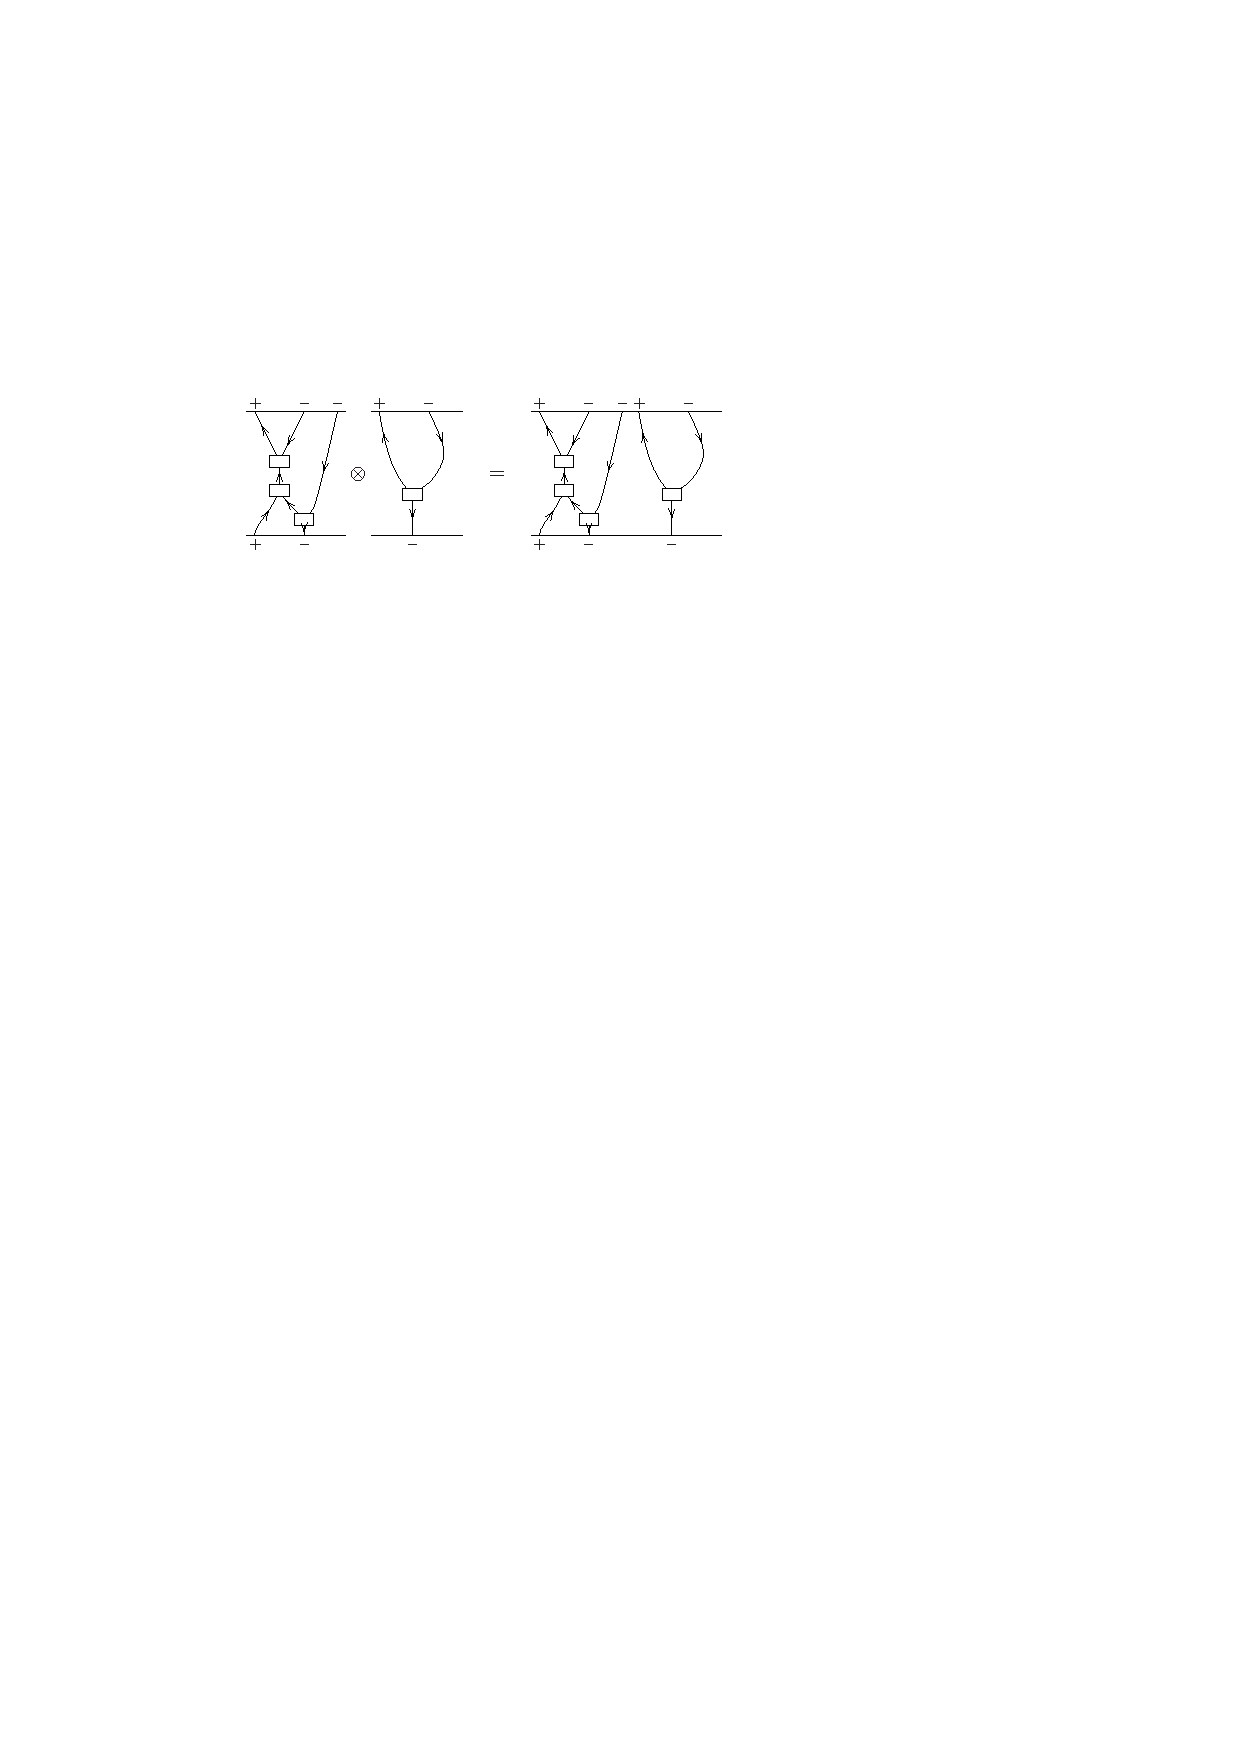
\includegraphics{fig-002}
  \end{equation*}
\caption{Tensor product of RT-diagrams.}
\label{fig:graph-otimes}
\end{figure}

Diagrams corresponding to directed braids on $n$  strands form a group
under the composition product, isomorphic to the semidirect product
$B_n \ltimes \setZ_2^n$.

By the above definitions, we can take the linear spans $\RTD(S,T)$ of
diagrams with given source $S$ and target $T$, as the $\Hom$-spaces of a
suitable category.
\begin{definition}
\label{dfn:diagrams-category}
$\RTD$ is the monoidal category which has finite sequences of $\pm1$ as
objects; the $\Hom$-space $\RTD(S,T)$ is the linear span of the set of
diagrams with source $S$ and target $T$.

Composition of morphisms is defined by bilinear extension of the
composition product $\circ$ (see \csref{dfn:graph-composition}).

The tensor product is given on objects by concatenation:
\begin{equation*}
  (\varepsilon_1, \ldots, \varepsilon_r) \otimes (\varepsilon'_1, \ldots, \varepsilon'_s) = (\varepsilon_1, \ldots, \varepsilon_r, \varepsilon'_1, \ldots, \varepsilon'_s),
\end{equation*}
and on morphisms by juxtaposition of diagrams (see
\csref{fig:graph-otimes}). 
\end{definition}

The category $\RTD$ is not braided, nor autonomous, nor balanced in
any obvious way: it is the deep result of Reshetikhin-Turaev
\cite{reshetikhin-turaev;ribbon-graphs}, Joyal-Street
\cite{joyal-street;tensor-calculus} and Freyd-Yetter
\cite{freyd-yetter;btc} that a quotient of it enjoys all these
structures; moreover, this result can be enhanced by considering
\emph{colored} graphs, and colors can be taken in any braided
autonomous tortile category.


\section{The category of RT-graphs}
\label{sec:rt-graphs}
Let $\Hom\RTD := \bigcup_{S,T \in \RTD} \RTD(S,T)$ be the set of all
morphisms in the category $\RTD$; $\Hom\RTD$ consists of all possible
RT-diagrams. Any RT-diagram can be considered as the planar projection
of a purely $1$-dimensional CW-complex equipped with some additional
structure.
\begin{definition}
  An (embedded) RT-graph\footnote{What is here called an ``RT-graph''
    corresponds to a ``homogeneous colored directed ribbon graph''
    (HCDR-graph) in the terminology of
    \cite{reshetikhin-turaev;ribbon-graphs}: the ``ribbon'' condition
    has been rephrased in terms of framing here, and the
    ``homogeneity'' is hidden in the requirement that $N_\ell$ satisfy
    $N_\ell(0) = N_\ell(1) = 1$. We do not need CDR-graphs (i.e., not
    homogeneous). Also, since we are ultimately going to consider
    coarser invariants than Reshetikhin and Turaev do, the definition
    of RT-graph has been adapted to suit a more combinatorial
    environment.} $\Gamma$ is a $1$-dimensional CW-complex embedded in $M
  = \setR \times [0,1] \times [0,1]$ together with
  \begin{itemize}
  \item for each edge, a choice of a direction;
  \item for each edge, a choice of a framing;
  \item for each vertev $v$, a partition of half-edges incident to it
    into disjoint totally-ordered subsets $\In(v)$ and $\Out(v)$.
  \end{itemize}
  In addition, we stipulate that $\Gamma \cap \partial M$ is a finite set --- call
  its points the \emph{endpoints} of $\Gamma$.  We say that $\Gamma$ has type
  $(p,q)$ iff $\Gamma \cap \partial M \subseteq \{ s_1, \ldots, s_p \} \cup \{ t_1, \ldots, t_q \}$.
\end{definition}
Extending a classical result of Reidmeister, Reshetikhin and Turaev
proved the following.
\begin{lemma}[\cite{reshetikhin-turaev;ribbon-graphs}]\label{lemma:moves}
  The set $\Hom\RTE$ of all isotopy classes (rel $\partial M$)\FIXME{Se
    dobbiamo considerare isotopie col bordo fisso allora non si pu{\`o}
    tagliare un grafo ad altezza generica\ldots vale la pena di essere
    estremamente precisi su questo punto?} of embedded
  RT-graphs is the quotient of the set $\Hom\RTD$ of RT-diagrams
  with respect to the equivalence relation generated by a finite set
  of graphical moves (Reidmeister-Reshetikhin-Turaev moves, see
  \csref{fig:rrt} or \cite{reshetikhin-turaev;ribbon-graphs} for a
  listing).
\end{lemma}
Henceforth, we say ``RT-graph'' to mean an element of $\Hom\RTE$ or an
isotopy class of embedded RT-graphs.\footnote{Reshetikhin and Turaev's
  original definition involved graphs with coupons (i.e., rectangles
  with a pair of preferred edges) as vertices and ribbons as the
  edges. Since the width of ribbons and the size of coupons do not
  matter under isotopy, we are ultimately left with $1$-dimensional
  edges with a framing, and with a partition of the edges incident to
  any given vertex.}
\begin{figure}[htbp]
  \centering
  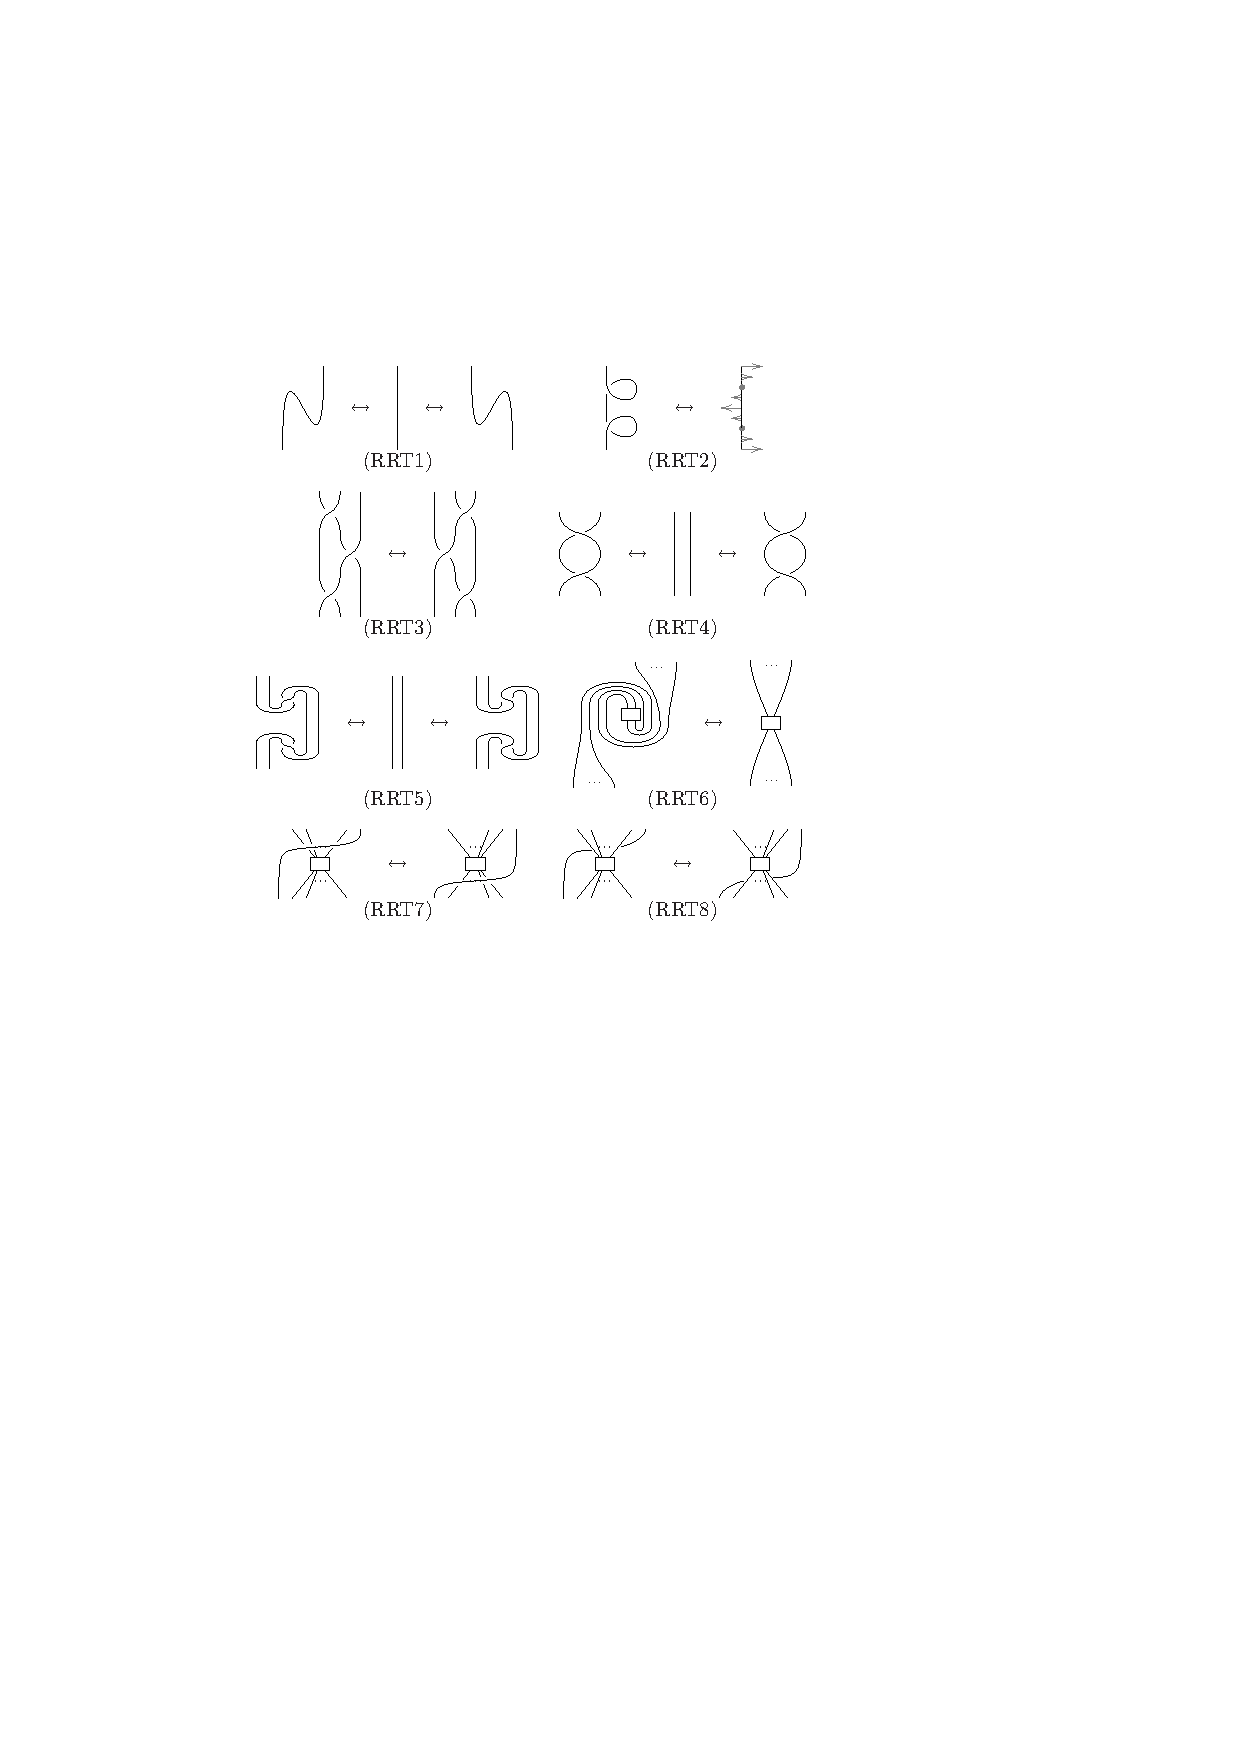
\includegraphics{fig-003}
    \caption{Reidmeister-Reshetikhin-Turaev moves for
      RT-diagrams. Note that move (RRT2) changes a trivial framing
      into a non-trivial (degree $1$) one.}
    \label{fig:rrt}
\end{figure}

It is clear that the operations $\circ$ and $\otimes$ on $\Hom\RTD$ induce
similar composition and tensor product operations on $\Hom\RTE$: any
two RT-graphs can be juxtaposed to form the tensor product $\otimes$ (see
\csref{fig:graph-otimes}) and a pair of graphs with matching input and
output legs can be stacked to form a new RT-graph (see
\csref{fig:graph-composition}).
\begin{lemma}[{\cite[lemmas 5.2 and 5.3]{reshetikhin-turaev;ribbon-graphs}}]
\label{thm:generators}
The set $\Hom\RTE$ of RT-graphs is generated thorugh $\circ$ and $\otimes$ from
the following elementary pieces ---an orientation must be
added to each strand!---, modulo the Reidmeister-Reshetikhin-Turaev
relations of \csref{fig:rrt}.
\begin{center}
%% Figura 5
  {%
    \begin{tabular}{cccccc}
      $\xy*!LC\xybox{(0,0);(0,1)**\dir{-}}\endxy$
      &
      $\xy*!LC\xybox{%
        \vcross~{(0,1)}{(1,1)}{(0,0)}{(1,0)}}\endxy$
      &
      $\xy*!LC\xybox{%
        \vcross~{(0,0)}{(1,0)}{(0,1)}{(1,1)}}\endxy$
      &
      $\xy*!LC\xybox{%
        \vloop~{(0,1)}{(1,1)}{(0,0)}{(1,0)}}\endxy$
      &
      $\xy*!LC\xybox{%
        \vloop~{(0,0)}{(1,0)}{(0,1)}{(1,1)}}\endxy$
      &
      $\xy*!LC\xybox{
        (0,1)*+[F]{\ };%
        (-1,0)**\dir{-},(-0.5,0)**\dir{-},%
        (0,0.5)*+{\ldots},(1,0)**\dir{-},%
        (-1,2)**\dir{-},(-0.5,2)**\dir{-},%
        (0,1.5)*+{\ldots},(1,2)**\dir{-},%
        }\endxy$
      \\
      (a) & (b) & (c) & (d) & (e) & (f)
    \end{tabular}
    }
\end{center}
\end{lemma}
A piece of type (a) is called a ``strand''; those of type (b) and (c)
are named ``crossings''; (d) and (e) are the ``coupling'' and the
``Casimir''; (f) is, plainly, a ``vertex''.
\begin{remark} \csref{thm:generators} just states that an
  RT-diagram is a composition of ``rows'' made of pieces of type
  (a)--(f). Generically, such rows will be made of one piece of type
  (b)--(f) padded with a number of strands (a) on the two sides.
\end{remark}

\begin{definition}
  $\RTE$ is the monoidal category whose arrows are elements of
  $\Hom\RTE$ with the composition law and tensor product induced as a
  quotient of $\Hom\RTD$.
\end{definition}
By the arrows-only description of a category (see \csref{cha:arrows}),
we can deduce that objects in $\RTE$ are finite sequences of signs $\pm1$.
Note that, for any such sequence $S$, the set $\RTE(S,S)$ contains the
directed braids group $B_n \ltimes \setZ_2^n$, so any braid is an
isomorphism in $\RTE$.

The category $\RTE$ has duals: for each object $S$, let $\rdl{S}$ be the
sequence obtained from $S$ by flipping it and reversing all the signs
---for instance, if $S = (+--)$ then $\rdl{S} = (++-)$---; let $\ev_S:
S\otimes\rdl{S} \to I$ be the only graph which connects corresponding signs
in $S$ and $\rdl{S}$ and has only local maxima of the height function
as critical points (see \csref{fig:ev}), finally, let $\coev_S : I \to
\rdl{S} \otimes S$ be the graph obtained by flipping $\ev_S$ both
horizontally and vertically. (See \textsl{(a)} and \textsl{(b)} in
\csref{fig:struct}.)

The category $\RTE$ is balanced by the family of isomorphisms $\theta_S: S
\to S$ defined by requiring that $\theta_{S\otimes T} := \theta_S \otimes \theta_T$ and
that $\theta_{(+)}$ be the straight line $\ell: [0,1] \ni t \mapsto (0,t,0) \in M$
with the degree $1$ framing $N_\ell: [0,1] \ni u \mapsto \exp 2\pi\I u \in
S^1$. (See \textsl{(c)} in \csref{fig:struct}.)

Finally, $\RTE$ is braided by the family of isomorphisms $\tau_{S,T}$
that swap the positions of $S$ and $T$, with directions chosen so to
match the signs on endpoints. (See \textsl{(d)} in
\csref{fig:struct}.)

\begin{figure}[thbp]
  \centering
  \begin{tabular}{cc}
    {\begin{tabular}{cc}
        $\rdl{S} \otimes S$
        &
        $\overbrace{\hspace{1.5cm}}^{\rdl{S}} \hspace{0.5cm}
        \overbrace{\hspace{1.5cm}}^S$
        \\
        ${\xy<0.5cm,0cm>:0, \ar(0,0);(0,3.5) ^{\coev_S} 
          _{\phantom{\coev_S}} \endxy}$
        &
        \includegraphics[scale=0.5]{coev}
        \\
        $I$
        &
      \end{tabular}}
    &
    {\begin{tabular}{cc}
        $I$
        &
        \\
        $\xy<0.5cm,0cm>:0, \ar(0,0);(0,3.5) ^{\ev_S} _{\phantom{\ev_S}} \endxy$
        &
        \includegraphics[scale=0.5]{ev}
        \\
        $S \otimes \rdl{S}$
        &
        $\underbrace{\hspace{1.5cm}}_{S} \hspace{0.5cm}
        \underbrace{\hspace{1.5cm}}_{\rdl{S}}$
      \end{tabular}}
    \\
    \textsl{(a)}
    &
    \textsl{(b)}
    \\[12pt]
    {\begin{tabular}{cc}
        S
        &
        S
        \\
        ${\xy<0.75cm,0cm>:0, 
          \ar(0,0);(0,3) ^{\theta_S} _{\phantom{\theta_S}}
          \endxy}$
        &
        ${\xy<1.125cm,0cm>:0,%
          (0,0);(0,2)**\dir{-},
          \ar@[grey] (0,0.00);(+0.50,0.00),
          \ar@[grey] (0,0.25);(+0.25,0.25),
          \ar@{-} (0,0.50)*[grey]{\bullet};(0,0.50),
          \ar@[grey] (0,0.75);(-0.25,0.75),
          \ar@[grey] (0,1.00);(-0.50,1.00),
          \ar@[grey] (0,1.25);(-0.25,1.25),
          \ar@{-} (0,1.50)*[grey]{\bullet};(0,1.50),
          \ar@[grey] (0,1.75);(+0.25,1.75),
          \ar@[grey] (0,2.00);(+0.50,2.00),
          (1,1.5)*{\ldots},
          (2,0);(2,2)**\dir{-},
          \ar@[grey] (2,0.00);(2.50,0.00),
          \ar@[grey] (2,0.25);(2.25,0.25),
          \ar@{-} (2,0.50)*[grey]{\bullet};(2,0.50),
          \ar@[grey] (2,0.75);(1.75,0.75),
          \ar@[grey] (2,1.00);(1.50,1.00),
          \ar@[grey] (2,1.25);(1.75,1.25),
          \ar@{-} (2,1.50)*[grey]{\bullet};(2,1.50),
          \ar@[grey] (2,1.75);(2.25,1.75),
          \ar@[grey] (2,2.00);(2.50,2.00),
          \endxy}$
        \\
        S
        &
        S
      \end{tabular}}
    &
    {\begin{tabular}{cc}
        $T\otimes S$
        &
        $\overbrace{\hspace{1.5cm}}^T \hspace{0.75cm}
        \overbrace{\hspace{1.5cm}}^S$
        \\
        $\xy<0.75cm,0cm>:0, \ar(0,0);(0,3) ^{\tau_{S,T}} _{\phantom{\tau_{S,T}}} \endxy$
        &
        \includegraphics[scale=0.75]{braid}
        \\
        $S\otimes T$
        &
        $\underbrace{\hspace{1.5cm}}_S \hspace{0.75cm}
        \underbrace{\hspace{1.5cm}}_T$
      \end{tabular}}
    \\
    \textsl{(c)}
    &
    \textsl{(d)}
  \end{tabular}
  \caption{The structure morphisms making $\RTE$ into a braided \textsl{(d)},
    autonomous \textsl{(a, b)}, tortile \textsl{(c)} category. The
    directions on each strand must be chosen according to the signs in
    $S$ and $T$. Note that the balancing $\theta_S$ is just the identity
    with a different framing.}
  \label{fig:struct}
\end{figure}

\begin{proposition}\label{thm:rt}
  The category $\RTE$ is braided, autonomous, and tortile.
\end{proposition}
\begin{proof}
  All the verifications reduce to checking that some RT-graph
  corresponding to a composition of the strcture morphisms is
  \emph{isotopic} to some other RT-graph, again composition of the
  structure morphisms ---for instance, move (RRT1) in \csref{fig:rrt}
  is the verification that $(\ev_{(\pm)}, \coev_{(\pm)})$ is a duality
  pair--- and this is easily done.
\end{proof}


\section{Graphical calculus on tortile braided tensor categories}
\label{sec:rt-gc}
Now let $\A$ be a tensor category. Define $\freemsc{\A}$ to be the
category whose objects are finite sequences $(A_1, \ldots, A_r; \varepsilon_1, \ldots,
\varepsilon_r)$ of objects in $\A$ and signs $\pm1$, whereas a morphism $(A_*,
\varepsilon_*) \to (B_*, \delta_*)$ is an element $f \in \A(A_1^{\varepsilon_1} \otimes \ldots \otimes
A_r^{\varepsilon_r}, B_1^{\delta_1} \otimes \ldots B_s^{\delta_s})$ --- recall that $A^1 = A$
and $A^{-1} = \rdl{A}$.  There is an obvious functor $\freemsc{\A} \to
\A$ defined on objects by $(A_1, \ldots, A_r; \varepsilon_1, \ldots, \varepsilon_r) \mapsto
A_1^{\varepsilon_1} \otimes \cdots \otimes A_r^{\varepsilon_r}$.
\begin{definition}
  An $\A$-colored RT-diagram $\Gamma$ is an RT-diagram together with:
  \begin{enumerate}
  \item an assignment of an object $A_\ell \in \A$ for each
    $\ell\in\Edges{\Gamma}$;
  \item an assignment of a morphism $f\in\A(\Src(v),\Tgt(v))$ for each
    vertex $v$ of $\Gamma$, where $\Src(v)$ and $\Tgt(v)$ are the
    sequences $(A_1, \ldots, A_r;\varepsilon_1, \ldots, \varepsilon_r)$ of objects and signs
    decorating edges in $\In(v)$ and $\Out(v)$.
  \end{enumerate}
  The source and the target of an $\A$-colored RT-diagram are defined
  analogously and are denoted $\Src_\A(\Gamma)$ and $\Tgt_\A(\Gamma)$ respectively.
\end{definition}
It is trivial to generalize \csref{dfn:diagrams-category} to
$\A$-colored RT-diagrams; call $\RTD[\A]$ the category of
$\A$-colored RT diagrams. $\Src{}_{\A}(\Gamma)$ and $\Tgt{}_{\A}(\Gamma)$ are
objects of $\freemsc{\A}$ for each $\A$-colored RT-diagram.
Obviously, $\circ$ and $\otimes$ are bilinear with respect to the vector space
structure on the $\Hom$-sets of $\RTD[\A]$. Any $\A$-colored
RT-diagram can be seen as the planar projection of an $\A$-colored
RT-graph and the following analogue of lemmas \ref{thm:generators}
and \ref{thm:moves} hold.
\begin{proposition}
\label{thm:rt1}
The set $\Hom\RTD[\A]$ of $\A$-colored RT-diagrams is generated thorugh
$\circ$ and $\otimes$ from the following elementary pieces (an orientation
must be added to each strand!):
\begin{center}
  %% Figura 7
  {%
    \begin{tabular}{cccccc}
      $\xy*!LC\xybox{(0,0)*+{A};(0,1)*+{A}**\dir{-}}\endxy$
      &
      $\xy*!LC\xybox{%
        \vcross~{(0,1)*+{B}}{(1,1)*+{A}}{(0,0)*+{A}}{(1,0)*+{B}}}\endxy$
      &
      $\xy*!LC\xybox{%
        \vcross~{(0,0)*+{B}}{(1,0)*+{A}}{(0,1)*+{A}}{(1,1)*+{B}}}\endxy$
      &
      $\xy*!LC\xybox{%
        \vloop~{(0,1)}{(1,1)}{(0,0)*+{A}}{(1,0)*+{A}}}\endxy$
      &
      $\xy*!LC\xybox{%
        \vloop~{(0,0)}{(1,0)}{(0,1)*+{A}}{(1,1)*+{A}}}\endxy$
      &
      $\xy*!LC\xybox{
        (0,1)*+[F]{f};%
        (-1,0)*+{A_1}**\dir{-},(-0.5,0)*+{A_2}**\dir{-},%
        (0,0.5)*+{\ldots},(1,0)*+{A_r}**\dir{-},%
        (-1,2)*+{B_1}**\dir{-},(-0.5,2)*+{B_2}**\dir{-},%
        (0,1.5)*+{\ldots},(1,2)*+{B_s}**\dir{-},%
        }\endxy$
      \\
      (a) & (b) & (c) & (d) & (e) & (f)
    \end{tabular}
    }
\end{center}
The set $\Hom\RTE[\A]$ of $\A$-colored RT-graphs is the quotient of
$\Hom\RTD[\A]$ with respect to the Reidmeister-Reshetikhin-Turaev
relations of \csref{fig:rrt}.
\end{proposition}

Let $\category{B}$ be a tensor category. A tensor functor
$\RTD[\A]\to{\category{B}}$ is uniquely specified if we define it on
the generators; it induces a tensor functor $\RTE[\A] \to \category{B}$
if it is compatible with relations (RRT1)--(RRT8).  In particular,
taking $\category{B}=\A$ we find the following.
\begin{theorem}[Reshetikhin-Turaev,
  \cite{reshetikhin-turaev;ribbon-graphs}]
  \label{thm:rt2}
  For any autonomous balanced braided tensor category $\A$, there is a
  tensor functor $Z_{\A}: \RTD[\A] \to \A$, mapping an object $(A_1,
  \ldots, A_r; \varepsilon_1, \ldots, \varepsilon_k) \in \RTD[\A]$ to $A_1^{\varepsilon_1} \otimes \dots \otimes
  A_k^{\varepsilon_k} \in \A$, and defined on generators of morphisms in
  $\RTD[\A]$ by
\begin{center}
  \everyxy={/r24pt/:}
  %% Figura 8
  {%
    \begin{tabular}{ccc}
      $\xy*!LC\xybox{%
        \vcross~{(0,1)*+{B}}{(1,1)*+{A}}{(0,0)*+{A}}{(1,0)*+{B}}}\endxy
      \mapsto \tau_{XY},$
      %\label{graph-cross+}
      &
      $\xy*!LC\xybox{%
        \vcross~{(0,0)*+{B}}{(1,0)*+{A}}{(0,1)*+{A}}{(1,1)*+{B}}}\endxy
      \mapsto \tau_{XY}^{-1},$
      %\label{graph-cross-}
      &
      $\xy*!LC\xybox{
        (0,1)*+[F]{f};%
        (-1,0)*+{A_1}**\dir{-},(-0.5,0)*+{A_2}**\dir{-},%
        (0,0.5)*+{\ldots},(1,0)*+{A_r}**\dir{-},%
        (-1,2)*+{B_1}**\dir{-},(-0.5,2)*+{B_2}**\dir{-},%
        (0,1.5)*+{\ldots},(1,2)*+{B_s}**\dir{-},%
        }\endxy \mapsto f$
      %\label{graph-morphism} 
      \\
      $\xy*!LC\xybox{%
        \vloop~{(0,1)}{(1,1)}{(0,0)*+{A}}{(1,0)*+{A}}}\endxy \mapsto
      \ev_{A},$
      %\label{graph-casimir}
      &
      $\xy*!LC\xybox{%
        \vloop~{(0,0)}{(1,0)}{(0,1)*+{A}}{(1,1)*+{A}}}\endxy \mapsto
      \coev_{A},$
      %\label{graph-coupling}
      &
      $\xy*!LC\xybox{(0,0)*+{A};(0,1)*+{A}**\dir{-}}\endxy \mapsto
      \id_X,$
      %\label{graph-id}
    \end{tabular}
    }
  \end{center}
where $\tau_{AB}$, $\ev_A$, $\coev_A$ are the structure maps in
$\A$, and $f$ is a morphism in $\A$; take the dual of an
object if the sign $\varepsilon$ on the corresponding edge is $-1$.

The tensor functor $Z_\A$ is invariant by the
Reidmeister-Reshetikhin-Turaev moves (RRT1)--(RRT8), so it induces a
faithful\FIXME{Non sono proprio sicuro che sia fedele!} tortile
braided functor $Z_\A: \RTE[\A] \to \A$.
\end{theorem}
\begin{remark}
By definition of a tensor functor, the following relations hold:
\begin{gather*}
  Z_{\A}(\Gamma\circ\Phi) = Z_{\A}(\Gamma) \circ Z_{\A}(\Phi), 
  \qquad 
  Z_{\A}(\Gamma\otimes\Phi) = Z_{\A}(\Gamma) \otimes Z_{\A}(\Phi),
  \\
  Z_{\A}(a\Gamma + b\Phi) = aZ_{\A}(\Gamma) + bZ_{\A}(\Phi).
\end{gather*}
\end{remark}

%%% Local Variables: 
%%% mode: latex
%%% TeX-master: "index"
%%% x-symbol-8bits: nil
%%% End: 



\RCSID $Id: operads.tex,v 1.1 2006/05/25 07:02:56 rmurri Exp $
%auto-ignore



\chapter{Operads}
\label{cha:operads}

Fix a differential graded $\k$-algebra $K$; the category of
$K$-dg-modules and their morphisms (not necessarily commuting with the
differential) is Abelian and symmetric monoidal with the tensor product
$\otimes := - \otimes_K -$.  In this section, we mainly follow
\cite{kriz-may;operads} for the definition of an operad.
\begin{definition}
  \label{dfn:operad}
  An operad ${\Oo}$ is a collection of $K$-modules $\{{\Oo}(n)\}_{n\geq0}$
  together with 
  \begin{enumerate}[i)]
  \item a unit map $\eta:K \to {\Oo}(1)$; 
  \item a right action of the symmetric group $\Perm{n}$ on ${\Oo}(n)$,
    for all $n\geq0$;
  \item composition maps ${\Oo}(n)\otimes{\Oo}(k_1)\otimes\cdots\otimes{\Oo}(k_n) \xrightarrow{\gamma_{n;
        k_1, \ldots, k_n}} {\Oo}(k)$ for all $n\geq0$ and $k = \sum k_s$; $\deg \gamma
    = 0$ as a map of graded modules.
  \end{enumerate}
  These data are required to satisfy the following compatibility
  relations.
  \begin{enumerate}
  \item\label{o-ass} The following \emph{associativity} diagrams
    commute, for all $n\geq0$, $k_s \geq0$, $j_{sr}\geq0$:
    \begin{equation}
      {\xymatrix{%
          {\Oo}(n) \otimes \bigl( \bigotimes_{s=1}^n {\Oo}(k_n) \bigr) \otimes \bigl( \bigotimes_{s=1}^n
          \bigotimes_{r=1}^{k_s} {\Oo}(j_{sr}) \bigr) 
          &
          {\Oo}(k) \otimes \bigl(\bigotimes_{s=1}^n \bigotimes_{r=1}^{k_s} {\Oo}(j_{sr}) \bigr)
          &
          k := \sum_s k_s
          \\
          &
          {\Oo}(j)
          \\
          {\Oo}(n) \otimes \biggl( \bigotimes_{s=1}^n \Bigl( {\Oo}(k_s) \otimes \bigl(
          \bigotimes_{r=1}^{k_s} {\Oo}(j_{sr}) \bigr) \Bigr) \biggr)
          &
          {\Oo}(n) \otimes \bigl( \bigotimes_{s=1}^n {\Oo}(j_s) \bigr)
          &
          j_r := \sum_{r=1}^{k_s} j_{sr}
          %%
          \ar@{<->}  "1,1";"3,1" _{\txt{signed \\ reordering}} 
          \ar "1,1";"1,2" ^{\gamma_{n; k_1, \ldots, k_n} \otimes \id}
          \ar "3,1";"3,2" ^{\id \otimes \bigotimes_{s=1}^n \gamma_{k_s; j_{s1}, \ldots,
              j_{sk_s}}} 
          \ar "1,2";"2,2" ^{\gamma_{k; j_{11}, \ldots, j_{nk_n}}}
          \ar "3,2";"2,2" _{\gamma_{n; j_1, \ldots, j_n}}
          }}
      \label{eq:o-ass}
    \end{equation}
    where the ``signed reordering'' acts is the appropriate
    composition of commutators in the symmetric category.
  \item\label{o-unit} The following \emph{unit} diagrams commute.
    \begin{equation}
      {\xymatrix{%
          {\Oo}(n)\otimes K\tp{n}
          \\
          & {\Oo}(n)
          \\
          {\Oo}(n) \otimes {\Oo}(1)\tp{n}
          \ar "1,1";"3,1" _{\id \otimes \eta\tp{n}}
          \ar "1,1";"2,2" 
          \ar "3,1";"2,2" _{\gamma_{n; 1, \ldots, 1}}
          }
        \qquad
        \xymatrix{%
          K \otimes {\Oo}(n)
          \\
          & {\Oo}(n)
          \\
          {\Oo}(1) \otimes {\Oo}(n)
          \ar "1,1";"3,1" _{\eta \otimes \id}
          \ar "1,1";"2,2" 
          \ar "3,1";"2,2" _{\gamma_{1; n}}
          }}
      \label{eq:o-unit}
    \end{equation}
  \item\label{o-perm} The following \emph{equivariance} diagrams
    commute, for $\sigma \in \Perm{n}$ and $\tau_s \in \Perm{k_s}$, the
    permutation $\sigma(k_1, \ldots, k_n) \in \Perm{k}$ permutes blocks of
    lengths $k_1$, \ldots, $k_n$ like $\sigma$ permutes letters; $\tau_1 \oplus \cdots
    \oplus \tau_n$ permutes letters in the $s$-th block as $\tau_s$ does:
    \begin{equation}
      {\xymatrix@C=36pt{%
          {\Oo}(n) \otimes {\Oo}(k_1) \otimes \cdots \otimes {\Oo}(k_n)
          & 
          {\Oo}(n) \otimes {\Oo}(k_{\sigma_1}) \otimes \cdots \otimes {\Oo}(k_{\sigma_n})
          \\
          {\Oo}(k)
          &
          {\Oo}(k)
          \ar "1,1";"1,2" ^{\sigma \otimes T_{\sigma^{-1}}}
          \ar "1,1";"2,1" _{\gamma_{n; k_1, \ldots, k_n}}
          \ar "1,2";"2,2" ^{\gamma_{n; k_{\tau_1}, \ldots, k_{\tau_n}}}
          \ar "2,1";"2,2" ^{\sigma(k_{\sigma_1}, \ldots, k_{\sigma_n})}
          }}
      \label{eq:o-perm1}
    \end{equation}
    and
    \begin{equation}
      {\xymatrix@C=48pt{%
          {\Oo}(n) \otimes {\Oo}(k_1) \otimes \cdots \otimes {\Oo}(k_n)
          & 
          {\Oo}(k)
          \\
          {\Oo}(n) \otimes {\Oo}(k_1) \otimes \cdots \otimes {\Oo}(k_n)
          &
          {\Oo}(k)
          \ar "1,1";"1,2" ^(.70){\gamma_{n; k_1, \ldots, k_n}}
          \ar "2,1";"2,2" _(.70){\gamma_{n; k_1, \ldots, k_n}}
          \ar "1,1";"2,1" _{\id \oplus (\tau_1 \otimes \cdots \otimes \tau_n)}
          \ar "1,2";"2,2" ^{\tau_1 \oplus \cdots \oplus \tau_n}
          }}
      \label{eq:o-perm2}
    \end{equation}
  \end{enumerate}
\end{definition}
Operads may be defined in any symmetric tensor category. For our
purposes, it will suffice to restrict always to the category of
$K$-dg-modules.

The prototypical operad is the \emph{endomorphism operad} $\EndOp[M]$ of some
$K$-dg-module $M$, which is defined by:
\begin{equation*}
  \EndOp[M](n) := \Hom( M\tp{n}, M).
\end{equation*}
The unit is given by the identity map $\id_M \in \Hom(M,M) =
\EndOp[M](1)$; the $\Perm{n}$-action is the (signed) permutation of
tensor product factors, and, finally, the maps $\gamma_{n; k_1, \ldots, k_n}$
are given by 
\begin{equation*}
  {\xymatrix{%
      \Hom(M\tp{n}, M) \otimes \Hom(M\tp{k_1}, M) \otimes \cdots \otimes \Hom(M\tp{k_n},
      M)
      \\
      \Hom(M\tp{n}, M) \otimes \Hom(M\tp{k}, M\tp{n})
      \\
      \Hom(M\tp{k}, M)
      \ar "1,1";"2,1" ^{\id \otimes (\text{$n$-fold tensor product of
          maps})}
      \ar "2,1";"3,1" ^{\circ}
      }}
\end{equation*}
It is trivial to verify that $\EndOp[M]$ is an operad.

A \emph{morphism of operads} $\phi: {\Oo}' \to {\Oo}''$ is a collection of
$K$-dg-modules morphisms $\{\phi_n: {\Oo}'(n) \to {\Oo}''(n)\}$ satisfying the
obvious compatibility conditions coming from diagrams
\eqref{eq:o-ass}--\eqref{eq:o-perm2}. 

\subsubsection{Signs in operads}
\label{sec:signs-operads}
The ``signed reordering'' of diagram \eqref{eq:o-ass} may appear as to
introduce an unnatural sign: infact it is not so, the reason being
that a Koszul sign is hidden into the $\gamma$'s, as the following example
shows.

Let $M$ be an $K$-dg-module, $A \in \Hom(M\tp{2}, M)$, $B_1 \in
\Hom(M,M)$ and $B_2 \in \Hom(M\tp2, M)$. According to the definition of
operad, $\gamma_{2; 1,2}(A \otimes B_1 \otimes B_2) \in \Hom(M\tp3, M)$, so we pick
$x_1 \otimes x_2 \otimes x_3 \in M\tp3$ and reckon:
\begin{equation*}
  y := (A \otimes B_1 \otimes B_2) (x_1 \otimes x_2 \otimes x_3) = A \otimes \bigl( (B_1 \otimes B_2)
  (x_1 \otimes x_2 \otimes x_3) \bigr),
\end{equation*}
so, by the Koszul sign convention,
\begin{multline*}
  y = A \otimes \bigl( (-1)^{x_1 B_2} B_1(x_1) \otimes B_2(x_2 \otimes x_3) \bigr) \\ 
  = (-1)^{x_1 B_2} A\bigl( (-1)^{x_1 B_2} B_1(x_1) \otimes B_2(x_2 \otimes x_3)
  \bigr).
\end{multline*}
Therefore,
\begin{equation}
  \label{eq:1}
  \gamma(A \otimes B_1 \otimes B_2) (x_1 \otimes x_2 \otimes x_3) = (-1)^{x_1B_2}  A\bigl( (-1)^{x_1 B_2} B_1(x_1) \otimes B_2(x_2 \otimes x_3) \bigr).
\end{equation}

Let us apply this to a particular case of \eqref{eq:o-ass}: pick $C_1,
C_2, C_3 \in \Hom(M,M)$, then use \eqref{eq:1} to walk \eqref{eq:o-ass}
bottom-up: first on the left-side path,
\begin{multline*}
  A\Bigl( B_1\bigl( C_1(x_1) \bigr), B_2\bigl(C_2(x_2), C_3(x_3)\bigr)
  \Bigr)  \\ = (-1)^{(x_1 + C_1)B_2} \gamma(A \otimes B_1 \otimes B_2) \bigl( C_1(x_1)
  \otimes C_2(x_2) \otimes C_3(x_3) \bigr)  \\ = (-1)^{C_1B_2 + x_1B_2 + x_1(C_2 +
    C_3) + x_2C_3}  \times \\ \gamma\bigl( \gamma(A \otimes B_1 \otimes B_2) \otimes C_1 \otimes C_2 \otimes C_3
  \bigr) (x_1 \otimes x_2 \otimes x_3),
\end{multline*}
then on the right-side path,
\begin{multline*}
  A\Bigl( B_1\bigl( C_1(x_1) \bigr), B_2\bigl(C_2(x_2), C_3(x_3)\bigr)
  \Bigr) \\ = (-1)^{x_2 C_3} A\bigl( \gamma(B_1 \otimes C_1) (x_1), \gamma(B_2 \otimes C_2
  \otimes C_3) (x_2 \otimes x_3) \bigr) \\ = (-1)^{x_2 C_3 + x_1(B_2 + C_2 + C_3)}
  \times \\ \gamma\bigl( A \otimes \gamma(B_1 \otimes C_1) \otimes \gamma(B_2 \otimes C_2 \otimes C_3) \bigr) (x_1 \otimes
  x_2 \otimes x_3).
\end{multline*}
Now we see that the sign $(-1)^{B_2C_1}$ coming from the reordering
\begin{equation*}
T_{(34)}: A \otimes B_1 \otimes B_2 \otimes C_1 \otimes C_2 \otimes C_3 \mapsto (-1)^{B_2 C_1} A \otimes
B_1 \otimes C_1 \otimes B_2 \otimes C_2 \otimes C_3
\end{equation*}
is the one needed to make diagram \eqref{eq:o-ass} commute.


\subsection{Algebras over operads}
\label{sec:algebras-over-operads}

Let $X$ be an $K$-dg-module, and ${\Oo}$ a fixed operad.
\begin{definition}
  A structure of ${\Oo}$-algebra on $X$ is an operad morphism ${\Oo} \to
  \EndOp[X]$ of ${\Oo}$ into the endomorphism operad of $X$. 
\end{definition}
So, elements in ${\Oo}(n)$ are interpreted as maps $X\tp{n} \to X$, that
is, they are $n$-ary operations on $X$. In the sequel we shall see how
to give a operadic formulation of common algebraic structures.

The following proposition encodes many well-known structure transfer
theorems. 
\begin{theorem}
  \label{prop:structure-transfer}
  Any morphism ${\Oo}\to{\Oo}'$ induces an ${\Oo}$-algebra structure on every
  ${\Oo}'$-algebra $X$, by means of the composition ${\Oo} \to {\Oo}'
  \to\EndOp[X]$.
\end{theorem}

In an equivalent manner, an ${\Oo}$-algebra structure on $X$, is given by
maps
\begin{equation*}
  \phi_n : {\Oo}(n) \otimes X\tp{n} \to X,
\end{equation*}
which satisfy associativity, unit and equivariance conditions coming
from diagrams \eqref{eq:o-ass}--\eqref{eq:o-perm2}, that we can
express by requiring the following diagrams to commute:
\begin{gather}
  \label{eq:o-alg}
  {\xyc\xymatrix{%
      {\Oo}(n) \otimes {\Oo}(k_1) \otimes \cdots \otimes {\Oo}(k_n) \otimes X\tp{k}
      &
      {\Oo}(k) \otimes X\tp{k}
      \\
      &
      X
      \\
      {\Oo}(n) \otimes \bigl({\Oo}(k_1) \otimes X\tp{k_1}) \otimes \cdots \otimes \bigl({\Oo}(k_n) \otimes
      X\tp{k_n})
      &
      {\Oo}(n) \otimes X\tp{n} 
      %%
      \ar@{<->} "1,1";"3,1"  _{\txt{signed \\ reordering}}
      \ar "1,1";"1,2" ^(.65){\gamma \otimes \id}
      \ar "1,2";"2,2" ^{\phi_k}
      \ar "3,2";"2,2" _{\phi_n}
      \ar "3,1";"3,2" _(.75){\id \otimes \phi\tp{k}}
      }\endxyc}
  \\
  {\xyc\xymatrix@C=36pt{%
      {\Oo}(n) \otimes X\tp{n}
      &
      {\Oo}(n) \otimes X\tp{n}
      \\
      {\Oo}(n) \otimes X\tp{n}
      & 
      X
      %%
      \ar "1,1";"1,2" ^{\id \otimes \varepsilon(\sigma)}
      \ar "1,1";"2,1" _{\sigma \otimes \id\tp{n}}
      \ar "1,2";"2,2" ^{\phi_n}
      \ar "2,1";"2,2" _{\phi_n}
      }\endxyc}
  \\
  {\xyc\xymatrix{%
      X
      &
      {\Oo}(1) \otimes X
      &
      X
      %%
      \ar "1,1";"1,2" ^(.35){\eta \otimes \id}
      \ar "1,2";"1,3" ^(.60){\phi_1}
      \ar@/_1pc/ "1,1";"1,3" _{\id_X}
      }\endxyc}
\end{gather}

\begin{example}[Free algebras over an operad] Fix an operad ${\Oo}$, and an
  $K$-dg-module $V$. Define the free ${\Oo}$-algebra $X := F_{\Oo}(V)$ by:
  \begin{equation*}
    X^p := {\Oo}(p) \otimes V.
  \end{equation*}
  In order to define the structure maps $\phi$, observe that 
  \begin{multline*}
    \bigl( {\Oo}(n) \otimes X\tp{n} \bigr)^p = {\Oo}(p) \otimes \bigoplus_{p_1 + \cdots + p_n =
      p} \bigl( ({\Oo}(p_1) \otimes X^{p_1}) \otimes \cdots \otimes ({\Oo}(p_n) \otimes X^{p_n})
    \bigr) 
    \\
    \simeq \bigl( {\Oo}(p) \otimes \bigoplus_{p_1 + \cdots + p_n =
      p} ({\Oo}(p_1) \otimes \cdots \otimes {\Oo}(p_n)) \bigr) \otimes (X\tp{n})^p,
  \end{multline*}
  so a direct sum of the maps $\gamma_{n; p_1, \ldots, p_n}$ will do the job.
\end{example}


\subsubsection{The operad of associative algebras}
\label{sec:operad-assoc}
If $X$ is an associative algebra, then a map $m: X\tp2 \to X$ is
defined, which satisfies the constraint
\begin{equation}
  \label{eq:ass}
  m(x_1, m(x_2, x3)) = m(m(x_1, x_2), x_3).
\end{equation}
Let us define an operad $\Ao$ which governs associative algebras; we
need an element $\mu \in \Ao(n)$ for every $n$-ary operation on $X$. Now,
the product of two elements $x_1 \otimes x_2 \mapsto m(x_1, x_2) =: x_1x_2$ is a
binary operation, but also the product in reverse order ($x_1 \otimes x_2
\mapsto m(x_2, x_1) =: x_2x_1$) is; moreover, we can form $n$-ary
operations composing product maps (e.g., $x_1 \otimes x_2 \otimes x_3 \otimes x_4 \mapsto
m(m(x_1, x_2), m(x_4, x_3)) = (x_1x_2)(x_3x_4)$).  The associativity
relation \eqref{eq:ass} tells us that any monomial $x_{\sigma_1} x_{\sigma_2}
\cdots x_{\sigma_n}$ defines a $n$-ary operation by composition of binary
products, independently of the way we put parentheses in it.
Therefore, we can state that $\Ao(n)$ is the $K$-module freely
generated by the set of all possible products of symbols $x_1, \ldots,
x_n$ with every $x_j$ appearing once and once only; for example,
\begin{equation*}
  \Ao(1) := K,
  \quad \Ao(2) := \lspan{ x_1x_2, x_2x_1}_K, 
  \quad \Ao(3) := \lspan{ x_{\sigma_1}x_{\sigma_2}x_{\sigma_3} : \sigma \in \Perm{3}}_K.
\end{equation*}
The $\Perm{n}$-action on $\Ao(n)$ consists in permuting the $x_j$'s.
The structure maps $\gamma_{n; k_1, \ldots, k_n}: \Ao(n) \otimes \Ao(k_1) \otimes \cdots \otimes
\Ao(k_n) \to \Ao(k_1 + \cdots + k_n)$ replace the $x_j$ in $\mu \in \Ao(n)$ by a
monomial $\mu_j \in \Ao(k_j)$, simultaneously replacing $x_l$ in $\mu_j$
with $x_{k_1 + \cdots + k_{j-1} + l}$.
  
The operad $\Ao$ is most easily described using a graphical notation.
Depict an element of $\Ao(n)$ as a \emph{binary} tree having $n$ leaves
(inputs) and one root (the output); the leaves are numbered, and
$\Perm{n}$ acts by permuting numbers on leaves. Such trees can be
easily seen to correspond to the meaningful insertion of $n-2$ pairs
of parentheses into a monomial $\mu \in \Ao(n)$.
\begin{center}
  \begin{tabular}{ccc}
    \begin{xytree}
      \branch{%
        \leaf{1}
        \leaf{2}
        }
    \end{xytree}
    &
    \begin{xytree}
      \branch{%
        \leaf{1}
        \branch{%
          \leaf{2}
          \leaf{3}
          }
        }
    \end{xytree}
    &
    \begin{xytree}
      \branch{%
        \branch{%
          \leaf{1}
          \leaf{3}
          }
        \branch{%
          \leaf{2}
          \leaf{4}
          }
        }
    \end{xytree}
    \\
    $x_1x_2$
    &
    $x_1(x_2x_3)$
    &
    $(x_1x_3)(x_2x_4)$
  \end{tabular}
\end{center}
The structure map $\gamma_{n; k_1, \ldots, k_n}$ simply grafts the tree $t_j
\in {\Oo}(k_j)$ onto the $j$-th input of $t \in {\Oo}(n)$ and renumbers the
leaves of $t_j$; for example,
\begin{equation*}
  \gamma \left\lgroup 
    \xytreec
      \branch{%
        \leaf{1}
        \leaf{2}
        }
    \endxytreec
    \otimes
    \xytreec
      \branch{%
        \branch{%
          \leaf{2}
          \leaf{3}
          }
        \leaf{1}
        }
    \endxytreec
    \otimes
    \xytreec
      \branch{%
        \branch{%
          \leaf{1}
          \leaf{3}
          }
        \branch{%
          \leaf{2}
          \leaf{4}
          }
        }
    \endxytreec
  \right\rgroup
  =
  \xytreec
    \branch{%
      \branch{%
        \branch{%
          \leaf{2}
          \leaf{3}
          }
        \leaf{1}
        }
      \branch{%
        \branch{%
          \leaf{4}
          \leaf{6}
          }
        \branch{%
          \leaf{5}
          \leaf{7}
          }
        }
      }
  \endxytreec
\end{equation*}
  
The whole family of numbered binary trees is generated by elements in
$\Ao(2)$ via the composition maps $\gamma$; infact,
\begin{equation*}
  \Ao(2) = \lspan{%
    \xytreec
      \branch{%
        \leaf{1}
        \leaf{2}
        }
    \endxytreec
    ,
    \xytreec 
      \branch{%
        \leaf{2}
        \leaf{1}
        }
    \endxytreec
    }.
\end{equation*}
What is more, the associativity relation \eqref{eq:ass} can be
rewritten as:
\begin{equation}
  \label{eq:ass-tree}
  \xytreec
    \branch{%
      \leaf{1}
      \branch{%
        \leaf{2}
        \leaf{3}
        }
      }
  \endxytreec
  =
  \xytreec
    \branch{%
      \branch{%
        \leaf{1}
        \leaf{2}
        }
      \leaf{2}
      }
  \endxytreec
\end{equation}
So, the operad $\Ao$ is the quotient of the family of binary
trees by relations of the form:
\begin{equation*}
  \gamma \left\lgroup
    T_0 \otimes \left\lgroup
  \xytreec
    \branch{%
      \leaf{1}
      \branch{%
        \leaf{2}
        \leaf{3}
        }
      }
  \endxytreec
  -
  \xytreec
    \branch{%
      \branch{%
        \leaf{1}
        \leaf{2}
        }
      \leaf{3}
      }
  \endxytreec
  \right\rgroup
  \otimes T_1 \otimes T_2 \otimes T_3 \right\rgroup 
\end{equation*}
where $T_0$, $T_1$, $T_2$ and $T_3$ are arbitrary binary trees.  It is
easy to check that these relations imply that any tree in $\Ao$ has
a representative such that left-wing branches have no ramification;
such trees will be called \emph{regular trees} in the sequel.

\begin{definition}
  The space $\Ao(n)$ is the $K$-linear span of the set of regular
  binary trees.  It is a dg-module with the trivial differential $D =
  0$.

  The collection $\{\Ao(n)\}$ forms an operad with the structure maps
  given by the grafting operation $\gamma$ and  the obvious $\Perm{n}$ action.
\end{definition}
It is an easy exercise to check the following.
\begin{theorem}
  Any associative algebra is an algebra over $\Ao$, and vice-versa.
\end{theorem}


\subsection{Modules over an operad algebra}
\label{sec:modules}
Fix an operad ${\Oo}$ and an ${\Oo}$-algebra $X$, and an $K$-module $M$. 
\begin{definition}
  A structure of $({\Oo}, X)$-module on $M$ is given by a collection of
  maps $\psi_n: {\Oo}(n+1) \otimes X\tp{n} \otimes M \to M$ which satisfy the following
  compatibility relations.
\begin{gather}
  \label{eq:o-2}
  {\xyc\xymatrix{%
      {\Oo}(n) \otimes {\Oo}(k_1) \otimes \cdots \otimes {\Oo}(k_n) \otimes X\tp{k-1} \otimes M & {\Oo}(k) \otimes
      X\tp{k-1} \otimes M
      \\
      {{\Oo}(n) \otimes \bigotimes_{j=1}^{n-1}\bigl({\Oo}(k_j) \otimes X\tp{k_j}) \otimes {\Oo}(k_n) \otimes
        X\tp{k_n-1} \otimes M}
      \\
      {\Oo}(n) \otimes X\tp{n-1} \otimes M & X
      %%
      \ar@{<->} "1,1";"2,1"  _{\txt{signed \\ reordering}}
      \ar "1,1";"1,2" ^(.65){\gamma \otimes \id_X\tp{k-1} \otimes \id_M}
      \ar "1,2";"3,2" ^{\psi_k}
      \ar "3,1";"3,2" _{\psi_n}
      \ar "2,1";"3,1" _(.75){\id \otimes \phi\tp{k-1} \otimes \psi_{k_n-1}}
      }\endxyc}
  \\
  {\xyc\xymatrix@C=48pt{%
      {\Oo}(n) \otimes X\tp{n-1} \otimes M
      &
      {\Oo}(n) \otimes X\tp{n-1} \otimes M
      \\
      {\Oo}(n) \otimes X\tp{n-1} \otimes M
      & 
      X
      %%
      \ar "1,1";"1,2" ^{\id_{\Oo} \otimes \varepsilon(\sigma) \otimes \id_M}
      \ar "1,1";"2,1" _{\sigma \otimes \id_X\tp{n-1} \otimes \id_M}
      \ar "1,2";"2,2" ^{\psi_n}
      \ar "2,1";"2,2" _{\psi_n}
      }\endxyc}
  \\
  {\xyc\xymatrix{%
      M
      &
      {\Oo}(1) \otimes M
      &
      M
      %%
      \ar "1,1";"1,2" ^(.35){\eta \otimes \id_M}
      \ar "1,2";"1,3" ^(.60){\psi_1}
      \ar@/_1pc/ "1,1";"1,3" _{\id_M}
      }\endxyc}
\end{gather}
\end{definition}

It is easy to check that modules over an $\Ao$-algebra are the usual
modules over an associative algebra.

Furthermore, one can define a notion of ``universal enveloping
algebra'' in an operadic context; the category of modules over an
${\Oo}$-algebra $X$ is naturally equivalent to that of modules over
the universal enveloping algebra $U_{\Oo}(X)$. As one would expect,
for $\Ao$ one gets the same standard notions of enveloping algebras.




%%% Local Variables: 
%%% mode: latex
%%% TeX-master: "index"
%%% End: 

\chapter{Python language syntax}
\label{chap:python}

\lstset{numbers=none}%

This chapter features a short introduction to the syntax of the
programming language Python, and an explanation of the commonly-used
constructs and idioms that may appear obscure.  This is by no means a
complete overview of the syntax, nor a formal definition of Python;
the \href{http://docs.python.org/3.1/}{official Python documentation}
\cite{python:docs, python:reference} should be consulted for this
purpose.

According to the
\href{http://en.wikipedia.org/wiki/Python_(programming_language)}
{Wikipedia article on Python} \cite{wikipedia:python}, ``Python is a
general-purpose high-level programming language. Its design philosophy
emphasizes code readability. Python claims to `[combine] remarkable
power with very clear syntax'. It has a relatively uncluttered visual
layout, uses English keywords frequently where other languages use
punctuation, and has notably fewer syntactic constructions than other
popular structured languages''.


\section{Basics of Python language syntax}
\label{sec:syntax}

Python is an \emph{imperative} programming language, meaning that
every Python program is a sequence of statements to be executed by the
computer.  Each statement must fit into a \emph{logical line}; a
logical line is the sortest sequence of consecutive display lines such
that all parentheses are balanced.  In other words, a statement ends
at the first newline character such that for every occurrence of
`"("', `"["', or `"{"' there is a matching occurence of
  the corresponding closing symbol.
\begin{lstlisting}
# single-line statement
print (21*2)

# the following statement is automatically continued
# until the newline following the last closing parenthesis
u = (1 + 4*x[2] 
       + 2*y[1 + n[42]]
       + z)
\end{lstlisting}
As one can see from the example above, the Python interpreter ignores
any character following `"#"' until the end of the line.  This
syntax is used to add explicative comments to the Python source code.
The Python interpreter completely ignores comments and blank lines
while reading a source file; that is, a Python program will have
\emph{exactly} the same behavior if all the comments and blank lines
are removed.

\subsection{Variables}
\label{sec:variables}

A variable name is \emph{bound} by assigning a value to it: e.g.,
"a=42".  Variables in Python are \emph{untyped}, that is, any
variable can hold an object of any type: "a=42" and "a=list()"
are both valid assignments. Variables in Python are also
\emph{mutable}, meaning that a single variable may be assigned a
different value several times over, within the same block of code.
For instance:
\begin{lstlisting}
a = 42 # an integer value
print(a)

a = "a character string"
print(a)

a = 3.1415926 # a floating-point number
print(a)
\end{lstlisting}


\subsection{Program blocks}
\label{sec:blocks}

A distinctive feature of Python is its use of whitespace to delimit
program blocks:\footnote{Note: the use of the word ``block'' here is
  not consistent with the meaning it is given in the Python Language
  Reference \cite{python:reference}.}  
Python mandates that statements belonging in the same sequence are
aligned with the same amount of whitespace from column 0 (the leftmost
one on the display).  The indentation must increase in the block after
a flow-control or function definition.\footnote{Python syntax also
  mandates that a colon \l{:} is the last non-whitespace character
  before a new block begins, so an effective rule of thumb is: if a
  line ends with a colon, the following one must increase
  indentation.}  A block ends upon encountering a statement with a
lesser indentation level (i.e., beginning closer to column 0).

For example, consider the following simple code:
\begin{lstlisting}
for x in range(10):
    # compute the square of x
    y = x*x
    # print it
    print y
# the following statement dedents, thus ending
# the body block of the "for" loop.
print "All done."
\end{lstlisting}
The assignment to variable "y" and the "print"
statement belong in the same code block (they body of the
"for" cycle), therefore both begin in column 2.  The
"for" and the last "print" statement belong in
the same sequence and therefore start at column 0. 


\section{Functions}
\label{sec:functions}

A Python function is a block of code dependent on a specified list of
named parameters.  A function is invoked by giving actual values to
the parameters; upon termination, functions return a value to their
caller. 

Python functions are defined using the "def" keyword; it must be
followed by the function name and a parenthesized list of parameters:
\begin{lstlisting}
def binomial(n, k):
  return factorial(n) / (factorial(k) * factorial(n-k))
\end{lstlisting}
A function is invoked by giving actual values to the parameters:
\begin{lstlisting}
x = binomial(4, 2)
print(x) # outputs `6'
\end{lstlisting}

Some of the parameters in a function can be given a default value, as
in the following example:
\begin{lstlisting}
def binomial(n, k=1):
  return factorial(n) / (factorial(k) * factorial(n-k))
\end{lstlisting}
Parameters with default values can be omitted from function
invocation; they will be given the default value declared in the
function definition:
\begin{lstlisting}
x = binomial(4) # == binomial(4, 1)
print(x) # outputs `4'
\end{lstlisting}


\section{Objects and classes}
\label{sec:objects}

Every datum that Python handles is an \emph{object}.  Strictly
speaking, an object is an aggregate data structure, consisting of data
fields (called ``instance variables'') and functions (called
``methods''); for the limited purposes of this exposition, it suffices
to say that an object is a group of variables and functions.

If $x$ is an object and $v$ is a variable name, then "$x$.$v$" is
the Python syntax used to refer to the instance variable $v$ within
$x$. Variables belonging in different object instances are independent
and can store different values.

If $x$ is an object and $f$ is a function name, then
"$x$.$f$($...$)" is said to ``invoke method $f$ on object $x$''
and is an alternate syntax for the function call \l{$f$($x$, $...$)}.

\subsection{Classes}
\label{sec:classes}

The type of an object determines what instance variables and methods
it has initially.  The type of an object is called its ``class'';
equivalently, one says that object $x$ is an \emph{instance} of class
$X$.  Classes are defined with the "class" statement:
\begin{lstlisting}
class Complex(object):
  def __init__(self, real, imag):
    self.real = real
    self.imag = imag
  def norm(self):
    return math.sqrt(self.real**2 + self.imag**2)
\end{lstlisting}
The above code defines a class "Complex" with two instance variables
"real" and "imag", and two instance methods "__init__" and
"norm".  Within the class definition, the keyword "self" denotes
the actual object on which the method is invoked: namely, if $x$ and
$y$ are both instances of class "Complex", then "$x$.norm()" and
"$y$.norm()" both execute the same code, with the variable "self"
bound to $x$ in the first case and to $y$ in the second. 

An instance of a class is created by invoking the class name as a
function, e.g.:
\begin{lstlisting}
x = Complex(1.0, 1.0)
\end{lstlisting}
The "__init__" method is executed when creating an instance of a
class, with the "self" parameter bound to the newly-created object.
The number of parameters following the class name in instance creation
must match those defined in the "__init__" method.

\subsection{Inheritance}
\label{sec:inheritance}

A class can \emph{inherit} its methods from other classes (named the
\emph{superclasses}): assume $x$ is an instance of class $X$, and $Y$ is a
superclass of $X$ defining a method $f$ then "$x$.$f$()" invokes the
method $f$ as defined in $Y$ (with "self" bound to $x$), unless $X$
also defines a method named $f$ (which would be invoked instead).

The ``inherits from'' relation is a partial order on the set of all
classes; on the transitive closure of a class $X$ this restricts to a
tree structure, with $X$ at the root: each time a method $f$ is
invoked on an instance of $X$, a depth-first search is done on classes
in the inheritance tree to find the definition of method $f$.

For example, consider the following code:
\begin{lstlisting}
class ComplexV(Complex):
  def unit_vector(self):
    return ComplexV(self.real/self.norm(), self.imag/self.norm())

x = ComplexV(2, 2)  # `x` is $2 + 2\I$
y = x.unit_vector() # `y` is $1/\sqrt{2} + 1/\sqrt{2}\I$
\end{lstlisting}
A class "ComplexV" is defined, which inherits from class
"Complex"; object of class "ComplexV" shall have a method
"unit_vector" defined in "ComplexV", and  methods "norm" and
"__init__" defined in "Complex" (by inheritance).  Indeed, the
definition of "unit_vector" invokes "self.norm()".

\subsection{Special methods}
\label{sec:special-methods}

Python defines some special method names; these methods, when defined,
are invoked with Python's natural operator syntax: e.g., if $x$
defines a method "__add__", then $x + y$ results in the method call
"$x$.__add__($y$)".  The full list of special methods and their
meaning is only available in the Python Language Reference
\cite{python:reference}; the ones used in the listings of
\csref{chap:algorithm} are:
\begin{itemize}
\item[{\ttfamily \_\_eq\_\_}] Used for testing object equality; if $x$ implements
  "__eq__", then \l{$x$ == $y$} actually runs "$x$.__eq__($y$)".
\item[{\ttfamily \_\_getitem\_\_}] If $x$ has a method "__getitem__", then the
  look-up expression \l{$x$[$k$]} is translated to the method call
  "$x$.__getitem__($k$)".
\item[{\ttfamily \_\_init\_\_}] Instance initialization, see \csref{sec:classes}.
\item[{\ttfamily \_\_len\_\_}] Returns the length (number of elements) in a
  container.
\item[{\ttfamily \_\_ne\_\_}] The opposite of "__eq__" (which see); if $x$
  implements "__ne__", then \l{$x$ != $y$} actually runs
  "$x$.__ne__($y$)"
\item[{\ttfamily \_\_repr\_\_}] Machine-readable printable representation of an
  object; returns a string, which should be a valid Python expression
  that yields a copy of the object when evaluated; called by
  "repr($x$)".
\item[{\ttfamily \_\_str\_\_}] Human-readable printable representation of an
  object; returns a string describing the instance; called by
  "str($x$)".
\end{itemize}


\section{Control flow constructs}
\label{sec:control-flow}

Python supports the usual control flow constructs
"if"/"else", "for", "while".

The "if"/"else" statements are used to select which of two
blocks of code will be executed.  The "else" part is optional and
can be omitted.  Cascaded "if"/"else" occurrences (to
select the execution of a particular block of instructions) are best
written using the "elif" keyword as a shorthand for 
`\verb"else: if:"'. 

The "while" statement repeatedly executes the ensuing code block;
the expression specified after the "while" keyword is evaluated
at the beginning of each execution cycle, if the result is boolean
false, then execution of the code block is aborted and the program
flows continues after the block following the "while" statement.
Therefore, if an expression evaluates to false at the first entrance
in the "while" block, the block is never executed.

The "for" statement repeatedly executes the ensuing code block,
each time binding the specified variables to a new value of the
sequence following the "in" keyword.
\begin{lstlisting}
for x in range(10):
  print(x)
\end{lstlisting}
The "range" function is provided as a convenience to specify
numerical integer sequences; by Python convention, the range is always
half-open: "range(10)" is the sequence of natural numbers $\{0,
1, \ldots, 9\}$.  More formally, we have:
\begin{align*}
  \text{\ttfamily range($n$,$m$)} &:= \{ x \in \setN : n \leq x < m \},
  \\
  \text{\ttfamily range($n$)} &:= \text{\ttfamily range(0,$n$)}
\end{align*}



\section{Containers}
\label{sec:containers}

In addition to the basic types (integers, floating-point numbers,
character strings), the Python language provides support for other
common data structures: lists, tuples ($t$-uples), dictionaries, and
sets.  These are collectively called \emph{container} types, as their
purpose is to store a collection of other objects.
There are two main operations supported by Python on standard
containers: \emph{iteration} and \emph{look-up}.

Iteration over a container is supported through the "for" loop
syntax:
\begin{lstlisting}
for item in container:
  # do something with item
  print(item)
\end{lstlisting}
The block of code following a \l{for ... in ...:} line will be
executed once for each item stored in the container; at each
iteration, the "for" variable will be bound to a different object in
the container.  Containers are said to be \emph{ordered} or
\emph{unordered}, depending whether iteration returns the objects in
the order they were added to the container (lists, tuples) or not
(dictionaries, sets).

Look-up returns the item stored at a particular position in the
container (in lists and tuples) or the one associated with a certain
\emph{key} (in dictionaries); sets do not support item look-up.  
Look-up is expressed by suffixing a container name with the index or key
within square brackets: if "L" is container name, and "p" is a
position, then \l{L[p]} represents the object stored in "L" at
position "p".

\subsection{Sets}
\label{sec:sets}

Python sets are an unordered collection of Python objects.  Sets are
\emph{mutable}: functions are available, to add and remove member objects to
a set, and to implement the most common set-theoretic operations.
Sets are defined by enclosing the list of member objects in braces
`\{' and `\}'; if an object is repeated several times in the list,
it will be stored only once in the "set" container:
\begin{lstlisting}
# define a set; duplicates will be removed
s1 = { 0, 1, "two", 1, 0 }

# same effect as the definition above
s2 = { 0, 1, "two" }
\end{lstlisting}
Python also allows defining sets with a syntax more similar to the
common mathematical writing:
\begin{lstlisting}
# define the set of the square numbers less than 100
s = { n*n for n in range(10) }

# same as above
s = set(n*n for n in range(10))
\end{lstlisting}
The general syntax of these expression (called ``set comprehensions''
in Python parlance) is:
\begin{lstlisting}
{ $f$ for $x$ in $X$ if $p$ }
\end{lstlisting}
where:
\begin{itemize}
\item[$x$] is any valid variable name;
\item[$X$] is any object that allows iteration (e.g., another
  set, a list, etc.);
\item[$f$] is any Python expression (i.e., a computation \l{n*n+1}) 
  that is only function of $x$;
\item[$p$] is a Python expression that evaluates to a
  Boolean truth value ("True"/"False") and only depends on $x$.
\end{itemize}
The above Python set comprehension translates to the current
mathematics notation:
\begin{equation*}
  \{ f(x) : x \in X \text{ such that } p(x) \text{ is true} \}
\end{equation*}
The "if"-clause with the boolean expression can be omitted, in which
case it is assumed to be "True" for all $x \in X$.

Sets do not allow look-up of elements, but allow iteration over the set
contents in a "for" loop:
\begin{lstlisting}
# define a set; duplicates will be removed
s = { 0, 1, "two", 1, 0 }

# iterate over the set contents
for item in s:
  print(item)
\end{lstlisting}

An \emph{immutable} variant "frozenset" is also provided;
"frozenset" instances cannot be modified once created.

                                                               
\subsection{Lists}
\label{sec:lists}

Python \emph{lists} store a sequence of values, and allow retrieving
each one by index-based look up.  Lists are like the ``arrays'' of
other programming languages, except that Python does not require all
values in a list to be of the same type.

List indices start at 0; negative indices denote elements from the end
of the list, so \l{l[-1]} is the last value in the list.  List
literals are delimited by a matching pair \l{[} and \l{]}, and the
items within must be separated by commas. For instance:
\begin{lstlisting}
# assign a list to the variable "l"
l = [1, 2, "three", 4.0]

# print the 3rd element -- indices start at 0
print l[2]
\end{lstlisting}
Lists can also be defined using a notation akin to the one used for
defining sets --- it is called \emph{list comprehensions}:
\begin{lstlisting}
# make a list of the first 10 square numbers
l1 = [ n*n for n in range(10) ]

# same as above, using a function-like constructor
l2 = list(n*n for n in range(10))
\end{lstlisting}

Lists are mutable objects: one can alter the values stored, append new
items or insert them in specified places, and delete portions of an
existing list.
\begin{lstlisting}
# alter a stored value, in-place
l[0] = "zero"

# append one item to a list
l.append(5)

# append another list
l.extend(["six", 7])

# insert a new value "1.5" between elements at position 1 and 2
l.insert(1, 1.5)

# delete the first 3 elements
del l[0:2]
\end{lstlisting}
It is possible to extract (and delete) \emph{slices} of a list, that is,
all items in a list associated with a range of consecutive indices.
The syntax is an extension of the index-based lookup: a slice is
denoted by the starting and ending index, separated by a colon
character \l{:} and enclosed by square brackets: the slice spans the
half-open interval $[\text{start index}, \text{end index})$.
\begin{lstlisting}
# create a list
l1 = [0, 1, 2, 3, 4, 5, 6]

# extract the first three elements
l2 = l1[0:3]
print l2

# now remove the slice "l2" from "l1"
del l1[0:3]
print l1
\end{lstlisting}


\subsection{Tuples}
\label{sec:tuples}

Python \emph{tuples} are exactly like lists: they allow an array of
different objects to be stored; tuples allow index-based lookup and
slicing. But, tuples are \emph{immutable}, so items cannot be
appended, inserted or deleted from a tuple.

Tuples can also be constructed using the comprehension syntax, but
only using the function-like syntax:
\begin{lstlisting}
# define a tuple of even numbers < 10
t = tuple(n for n in range(10) if (n % 2 == 0))
\end{lstlisting}


\subsection{Dictionaries}
\label{sec:dicts}

Python dictionaries implement a general (finite) mapping: they
associate an object with an (arbitrary) value.  Elements in the
mapping domain are called dictionary \emph{keys}; objects in the
codomain are called dictionary \emph{values}.  Python objects used as
keys must be immutable; this is one reason for having distinct mutable
and immutable versions of standard containers.

Python syntax for working with dictionaries is akin to the syntax used
for manipulating lists, the only difference being that dictionaries
are constructed by enclosing \l{key:value} pairs in braces:
\begin{lstlisting}
# define a dictionary
f = { "zero":0, "one":1, "two":2, "three":3 }
\end{lstlisting}
A dictionary can also be defined using the comprehension syntax,
akin to sets, but the defining expression must have the form
\l{$k$:$v$} where $v$ is the value to be associated to key $k$:
\begin{lstlisting}
# map each integer < 10 to its square
f = { n:(n*n) for n in range(10) }

# same as above, with a function-like constructor
f = dict(n:(n*n) for n in range(10))
\end{lstlisting}

Dictionaries support look-up using a syntax akin to the one used for
lists, but the look-up key can be any valid Python object:
\begin{lstlisting}
# lookup an element by key
print (f["one"])
\end{lstlisting}
Looking up a key which is not in the dictionary domain raises an
exception of type "KeyError".

Dictionaries are \emph{mutable} objects, new mappings can be added or
old ones can be replaced:
\begin{lstlisting}
# add a new mapping: "four" $\mapsto$ 4
f["four"] = 4

# ...change it... 
f["four"] = 4.0

# ...and delete it!
del f["four"]
\end{lstlisting}

Dictionary objects support iteration over keys, values, and over (key,
value) pairs:
\begin{lstlisting}
# iterate over dictionary keys
for k in f.iterkeys(): 
    print("dictionary key: ", k)

# iterate over dictionary values
for v in f.itervalues(): 
    print("dictionary value: ", v)

# iterate over (key, value) pairs
for (k, v) in f.iteritems(): 
    print("key ", k, "has value", v)
\end{lstlisting}
Using the comprehension syntax and iteration, it is easy to invert a
mapping:
\begin{lstlisting}
# define `g` as the inverse of `f`
g = { v:k for (k, v) in f.iteritems() }
\end{lstlisting}


\section[Exception handling]{Exception handling: \l{try}/\l{except}/\l{finally} statements}
\label{sec:try-except-finally}

Exceptions are a language runtime construct to abort current function
execution, usually to signal an error.  If a block of Python code
cannot perform its function, it would \emph{raise} and exception:
current execution is aborted and control is returned to the calling
function.  This is searched for an \emph{exception handler}; if none
is found, the process continues recursively, inspecting the calling
function's caller for an exception handler.  If no exception handler
could be found across the whole call stack, the Python program aborts
execution.

The "try"/"except"/"finally" statements
are used to define exception handlers for a block of code.  The code
block following the "try" statement is executed; if it
raises an exception, then each "except" clauses immediately
following is inspected: if the type of the exception being raised
matches the type specified in the "except" clause, then the
code block following "except" is executed. The code block
following an "except" statement can raise a new exception
(or re-raise the one it caught); if no exception is raised, execution
continues with the statement that follows the
"try"/"except".  The code block following
"finally" is \emph{always} excuted before control leaves the
"try"/"except" clauses (in either way, that is,
after a "try"/"except" block completed with no
errors, or before returning control to the caller function because
another exception has been raised).

In the following example, the "a[42]" value lookup may
raise an exception of type "KeyError"; if this happens,
code in the "except" block will assign a default value to
"b".
\begin{lstlisting}
try:
    b = a[42]
except KeyError:
    # `a` has no value in the "42" position; 
    # assign a default value to `b`
    b = 0

# execution continues here
print (b)
\end{lstlisting}
                     

\subsection{The {\l pass} statement}
\label{sec:pass}

Python syntax does not allow to specify an empty block of code. There
is thus a special "pass" statement that performs no
computational operation, and is used to define ``no-op'' blocks.

The main use of "pass" is in combination with an
"except" statement, to ignore a particular error condition:
\begin{lstlisting}
try:
  print (a[42])
except KeyError:
  pass # ignore error if `a` has no item "42"
\end{lstlisting}


%%% Local Variables: 
%%% mode: latex
%%% TeX-master: "index"
%%% End: 

% LocalWords:  boolean


%%
%% Bibliografia
%%
\bibliography{math,tech}
\bibliographystyle{halpha}


\backmatter

\end{document}

%%% Local Variables: 
%%% mode: latex
%%% TeX-master: t
%%% End: 
